\section{Introduction%
         \label{sec:introduction}}

The progress in image recognition in the last two decades has been nothing short of astonishing, not least due to the success of CNNs (Convolutional Neural Networks) (\cite{LeCun1999-ff}, \cite{Alom2018-yo}). While ML (Machine Learning) was mostly restricted to facial and handwritten character recognition prior to the 2000s in this area, a wide variety of new, significantly more complex problem domains have been opened up since then. Object classification and localization has emerged as a major field of computer vision with popular datasets such as ImageNet boasting multiple millions of high-resolution color samples of over 20.000 different categories (\cite{Deng2009-iz}). Automated evaluation of aerial and satellite images has become a backbone for cartography and environmental surveillance. Computer vision is increasingly employed for quality assessment in industry. Furthermore, image recognition has been extended from static images to real-time classification and tracking of objects in video streams. Popular applications for the latter include e.\,g.\ pose and action recognition and obstacle identification to list only a few examples.

However, as a consequence of the ongoing endeavor to solve evermore complex tasks, many modern models can't be economically feasibly trained anymore without computing capacities that necessitate access to datacenters or cloud platforms. While this is neither a completely novel nor in itself negative development, it does effect a drastic reduction in practical applicability and facilitates an increasing oligopolization of the DL (Deep Learning) industry as well as research in favor of those with access to more resources and / or data. This is further catalyzed by the inherent limitation of DL regarding the impossibility to refactor once learnt knowledge and the requirement to retrain the whole model each time a shift in the data base occurs.

Moreover, the decision-making process of conventional neural networks is difficult to comprehend due to their inherent nature. The latter is, however, becoming more and more important as such systems are increasingly employed in safety-critical applications such as autonomous driving or for predictions with high economic implications.

To address these shortcomings, we propose the modularization of neural networks in abstraction of the well-known "divide and conquer" principle from computer science. Similar approaches have been repeatedly investigated for different partial aspects of the described problem, e.\,g.\ in \cite{Jacobs1991-fo}, \cite{Yan2015-go} and \cite{Roy2020-rv}; with this work, however, we consider a different perspective and try to raise general awareness for this method.

Specifically, we hypothesize that by dividing neural networks into sparsely interconnected submodules that can be trained and invoked independently of each other in adherence to the inherent structure of the task resp.\ the data base and that each only learn a subspace of the composite problem space, the theoretically minimally necessary computing power for training and inference is drastically reduced. As they are self-contained, the individual modules can also be retrained stand-alone if e.\,g.\ a distributional shift in parts of the data base occurs or more samples of a hitherto underrepresented class become available subsequent to the initial training, making this kind of models well-suited for operation in dynamic fields of application. Additionally, as the modules of the resulting meta-network are naturally less specialized than the composite network, they become more accessible to transfer learning and it becomes easier to refactor knowledge.

\pagebreak

\begin{figure}[htb]
    \centering
	    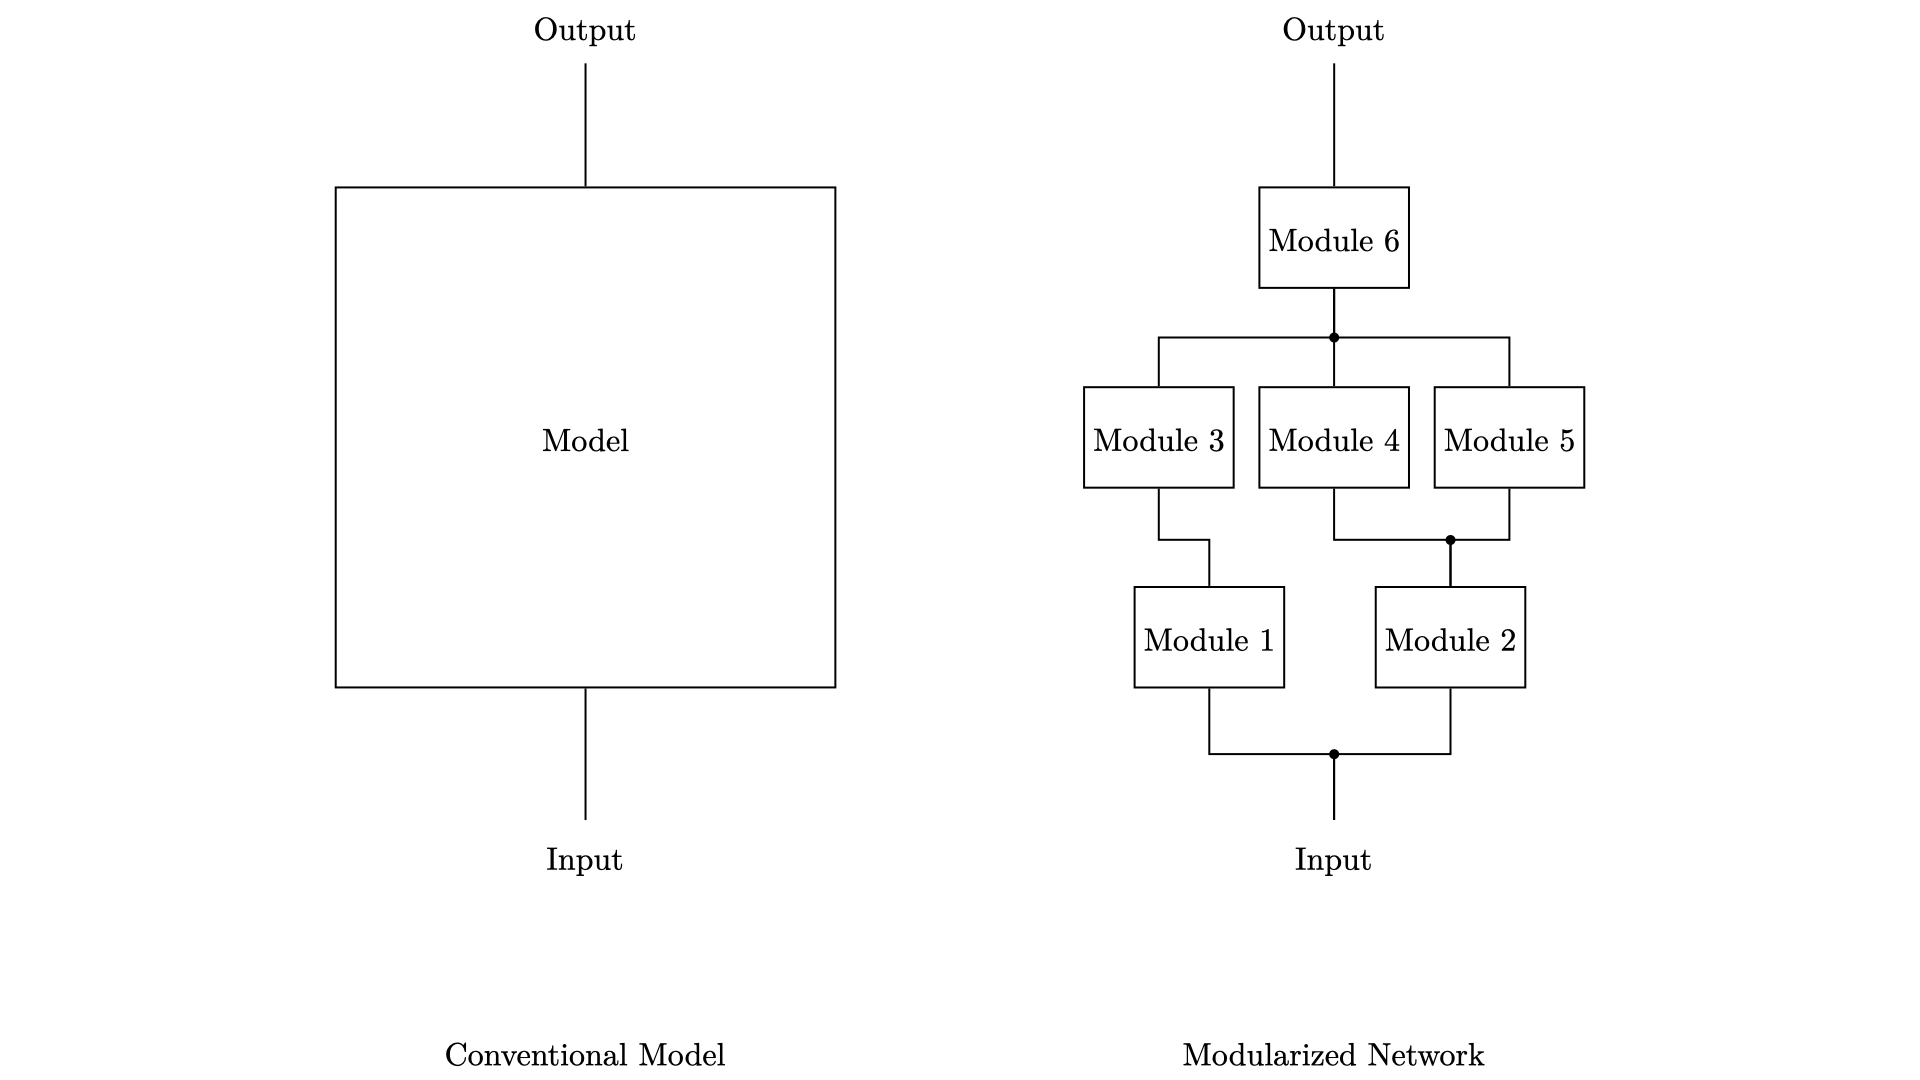
\includegraphics[width=\textwidth, trim=250 0 250 0, clip]{thesis/graphics/graphics/basic_concept.jpeg}
    \caption{Conventional ML models are black boxes after training. While the individual submodules of a composite network are equally obscure, the availability of intermediate predictions and the explicit definition of inter-module relationships facilitates behavioral comprehensibility.}
    \label{fig:modularization_basic_concept}
\end{figure}

As a positive ancillary effect, modularization simplifies the interpretability of the model's decision making process since humans equally tend to decompose complex problems into simpler sub-problems; hence, forecasts based on several iterative sub-decisions are easier to comprehend than monolithic predictions without intermediate results.

In this work, we examine the central question whether it is possible to decompose an existing monolithic model to obtain the above properties while at the same time retaining an acceptable degree of performance. We do not answer if it is generally possible to modularize any arbitrary model without loss of performance at all, nor do we derive bounds with regard to the latter. Generally, we assess the approach on a qualitative basis. In this, we do furthermore restrict our considerations to the most common forms of decomposition due to the limited scope of this work.

While the presented concepts are theoretically transferable to arbitrary models, in this work we limit our focus to DAGs (Directed Acyclic Graphs), in particular CNNs as a subcategory of neural networks. We provide a theoretical foundation and investigate the approach experimentally using different scenarios from the field of object classification to answer the following secondary questions:

\pagebreak

\begin{enumerate}
    \item How does modularization affect the learning behavior and detection rate of a model?
    \item How are decomposition and error rate of a network related?
    \item Are modularized models less stable than monolithic models?
\end{enumerate}

The remaining chapters are structured as follows: First, related works are introduced in section \ref{sec:related_work} and distinguishing aspects of this thesis are highlighted. Afterwards, two different higher-level perspectives on the modularization of ML models are presented and advantages and disadvantages of this approach are discussed from different points of view. Chapter \ref{sec:compnet} provides a theoretical analysis of decomposition as a technique as well as of the nature of errors induced by this method. Furthermore, a heuristic is provided to estimate the impact of a particular form of modularization on a model. Subsequently, three experiments are conducted in which performance and robustness of a model composed from multiple submodules are compared to a conventional neural network on different tasks from the field of image recognition. The work is concluded by a summarizing discussion of the results and an outlook on potential topics for future research in this area in section \ref{sec:conclusion}.

\cleardoublepage

\section{Related Work%
         \label{sec:related_work}}
         
The idea of composing a single model from multiple submodules has been around since the late 80s. Initial approaches to combine multiple learners originated from the domain of competitive learning, mainly born as an approach to overcome the limitations of computational resources that served as the primary bottleneck in ML at that time.

Early works such as \cite{Jacobs1991-fo} and \cite{Jacobs1991-rz} develop "divide and conquer" strategies to have different networks compete for subspaces of the domain, facilitated by gating networks that learn to dynamically switch between the submodules depending on the input. The authors argue that such an approach not only decreases hardware requirements but also increases learning speed and interpretability, reduces spatial and temporal crosstalk and leads to better generalization.

Adopting a similar philosophy, \cite{Jordan1994-gn} derive a stochastic framework for the "divide and conquer" approach; i.\,e.\ the model is trained using a variant of the EM (Expectation Maximization) algorithm to learn a mixture of probabilities from which the final result is then drawn. Making use of the Bayesian nature of the learned transformation, the authors are able to define lower bounds on the learning rate of the composed network to guarantee convergence which is also the main advantage of the approach.

Following a different paradigm, \cite{Pollack1987-pe} proposes a two component model consisting of a conventional MLP (Multi Layer Perceptron) and an additional context network that acts on the weights of the former and dynamically alters them before each forward-pass. The authors derive a modified version of the traditional backpropagation algorithm established by \cite{Rumelhart1986-jr} that enables the training of both submodules at the same time.

Early general studies on consensus theory in non-competitive modular systems can be found in \cite{Benediktsson1992-bl} and \cite{Xu1992-hp}. However, in contrast to the aforementioned approaches that mainly aim to increase resource effectiveness during learning, these works focus on the combination of different independently trained learners to reduce uncertainty and error rates when compared to the individual composing submodules. The latter concept has since then gained traction in a multitude of areas in ML and is used in various contemporary techniques such as Boosting, Bagging, Ensemble-building, etc. An overview of the fields in which modularization is employed for task-independent performance boosting today can e.\,g.\ be found in \cite{Alpaydin2019-nh}.

Most recent findings in the form of \cite{Filan2020-nx} furthermore suggest that neural networks in general tend to naturally form modular clusters when being trained using modern regularization techniques such as Pruning or Dropout and might thus be inherently accessible to modularization.

Concerning task-specific developments leveraging modularization, especially in image recognition, composed approaches have been widely discussed since the late 2000s. Already earlier works such as \cite{Zweig2007-oo} hypothesize that learners trained on different label hierarchy levels are incentivized to learn different representations of the same objects and that a combination of the individual predictions leads to improved performance similar to Ensembles. Yet, due to a lack of benchmarking possibilities, datasets used for experimentation were mostly individually assembled, inherently biased in favor of the composed approach (mainly because of the natural tendency to include only meta-classes with a disproportionately high decision boundary) and hardly comparable. However, since the establishment of publicly accessible, large-scale datasets with multiple label hierarchy levels such as CIFAR100 or ImageNet in the last decade, this paradigm has become increasingly popular in research.

E.\,g.\ \cite{Yan2015-go} propose a network composed of multiple template models. They employ unsupervised learning techniques to identify natural clusters of alike classes and train one building block model for each meta-concept found this way. Thereby the authors aim to maximize the decision boundaries between categories and optimize the usage of modeling capacity per individual module. Even though their comparative results are arguably disputable as they benchmark their modular network against a single of the composing template models which naturally has much less modeling capacity as well as a smaller memory footprint and execution time, their work suggests the validity of the approach and devises different techniques to further reduce hardware requirements for composed models.

A very recent publication originating from a different point of view by \cite{Roy2020-rv} employs tree-like, dynamically growing structures of CNNs to combat what the authors denote as "catastrophic forgetting" in image recognition, i.\,e.\ networks forgetting learned patterns when they are retrained on new data. Furthermore, the authors argue that a modular structure facilitates expendability and adaptability of DL models for situations where new data becomes steadily available or a constant distributional shift takes place as is the case in many real-world scenarios.

Similar to several of the aforementioned approaches, we aim to leverage modularization to facilitate the practical applicability of ML, especially DL, in various respects. However, the central question that we try to answer is whether it is possible to decompose an existing monolithic model to obtain a more versatile structure while at the same time retaining an acceptable degree of performance. I.\,e.\ what distinguishes our work is that we do not assess modularization as an extension of but rather as an alternative to conventional models. In that, our perspective fundamentally differs from related works.

Furthermore, we do not focus on any specific form of decomposition but rather aim to assess the fundamental concept as well as how the technique affects learning and predictive behavior of a model in general. In particular, we perform a benchmark with a comparable monolithic model to examine which approach makes more efficient use of the same modeling capacity. A further distinguishing aspect consists in the evaluation of practically relevant criteria such as error propagation and robustness (i.\,e.\ stability) of composed networks in an effort to not only provide indications concerning if, but also how much modularization is worth employing.

\cleardoublepage

\section{Motivation and Higher-Level Considerations%
         \label{sec:motivation}}
         
In theory, modular design has various advantages over conventional monolithic approaches with regard to practical applicability in many scenarios. In the following, a comparative overview of the different aspects affected by model decomposition is given. In doing so, two different perspectives are presented. First, a (software) architectural point of view is taken, i.\,e.\ the implications of modularization on the network as a program / a piece of source code such as scalability or exchangeability are considered. Secondly, aspects motivated from conventional Machine Learning are discussed.

\textbf{Architecturally motivated:} When considering the inherent software-nature of any model, decomposition has several advantages in comparison to monolithic approaches. In this, they are similar to most other complex software systems which can -- when done correctly -- greatly benefit from modularization with regard to practical applicability. E.\,g.\ \cite{Parnas1971-yk} and \cite{Parnas1971-xy} describe various advantages of modular programming in addition to general aspects of design methodology, whereas \cite{Page-Jones1996-vv} proposes structured design to conquer the complexity of large systems. \cite{Brooks1995-wm}, again, argues modular design to be beneficial from a managerial perspective in the process of software development. In this regard, aspects of particular interest for ML models are:

\begin{itemize}
    \item \textbf{Exchangeability:} Consider a ML model that is part of a business-critical process. Now imagine a scenario where changes to the model have to be made, e.\,g.\ because of domain specific shifts of the input distribution, a new model version with improved performance becomes available, or simply because one of the components involved in hosting the former needs to be patched due to security concerns. In the case of a conventional monolithic model, this implies that the whole business process has to be shut down, resulting in high economic cost. However, for a network composed of multiple submodules it is possible to perform the updates incrementally one module at a time.
    \item \textbf{Modifiability:} Assuming a sensible modularization (i.\,e.\ adhering to principles of low coupling and high cohesion as described by \cite{Stevens1974-rf}), the resulting composed network is prone to modifications in that changes are locally restricted in their scope of effect. Consider e.\,g.\ the case where a new class is to be added to the output of a model. Now, instead of having to modify and retrain the whole network, programmatic changes only need to be made to the submodules of the last layer (or the last two layers, depending on the architecture).
    \item \textbf{Parallelizability:} With a model composed of multiple submodules, it is possible to parallelize the two most time consuming steps in the development of ML models, training and fine tuning. Since they apply module wise, both can be performed for all constituting elements at the same time. I.\,e.\ even though there are more parts to be considered than for a monolithic model, each individual one is simpler and training and fine tuning are generally faster given sufficient computing resources. Especially in business scenarios, manpower can be utilized much more efficiently this way.
    
    \item \textbf{Scalability:} Modularization directly facilitates scalability of software systems. This again proves beneficial in various respects for ML models:
        
\pagebreak
        
\begin{figure}[tb]
    \centering
	    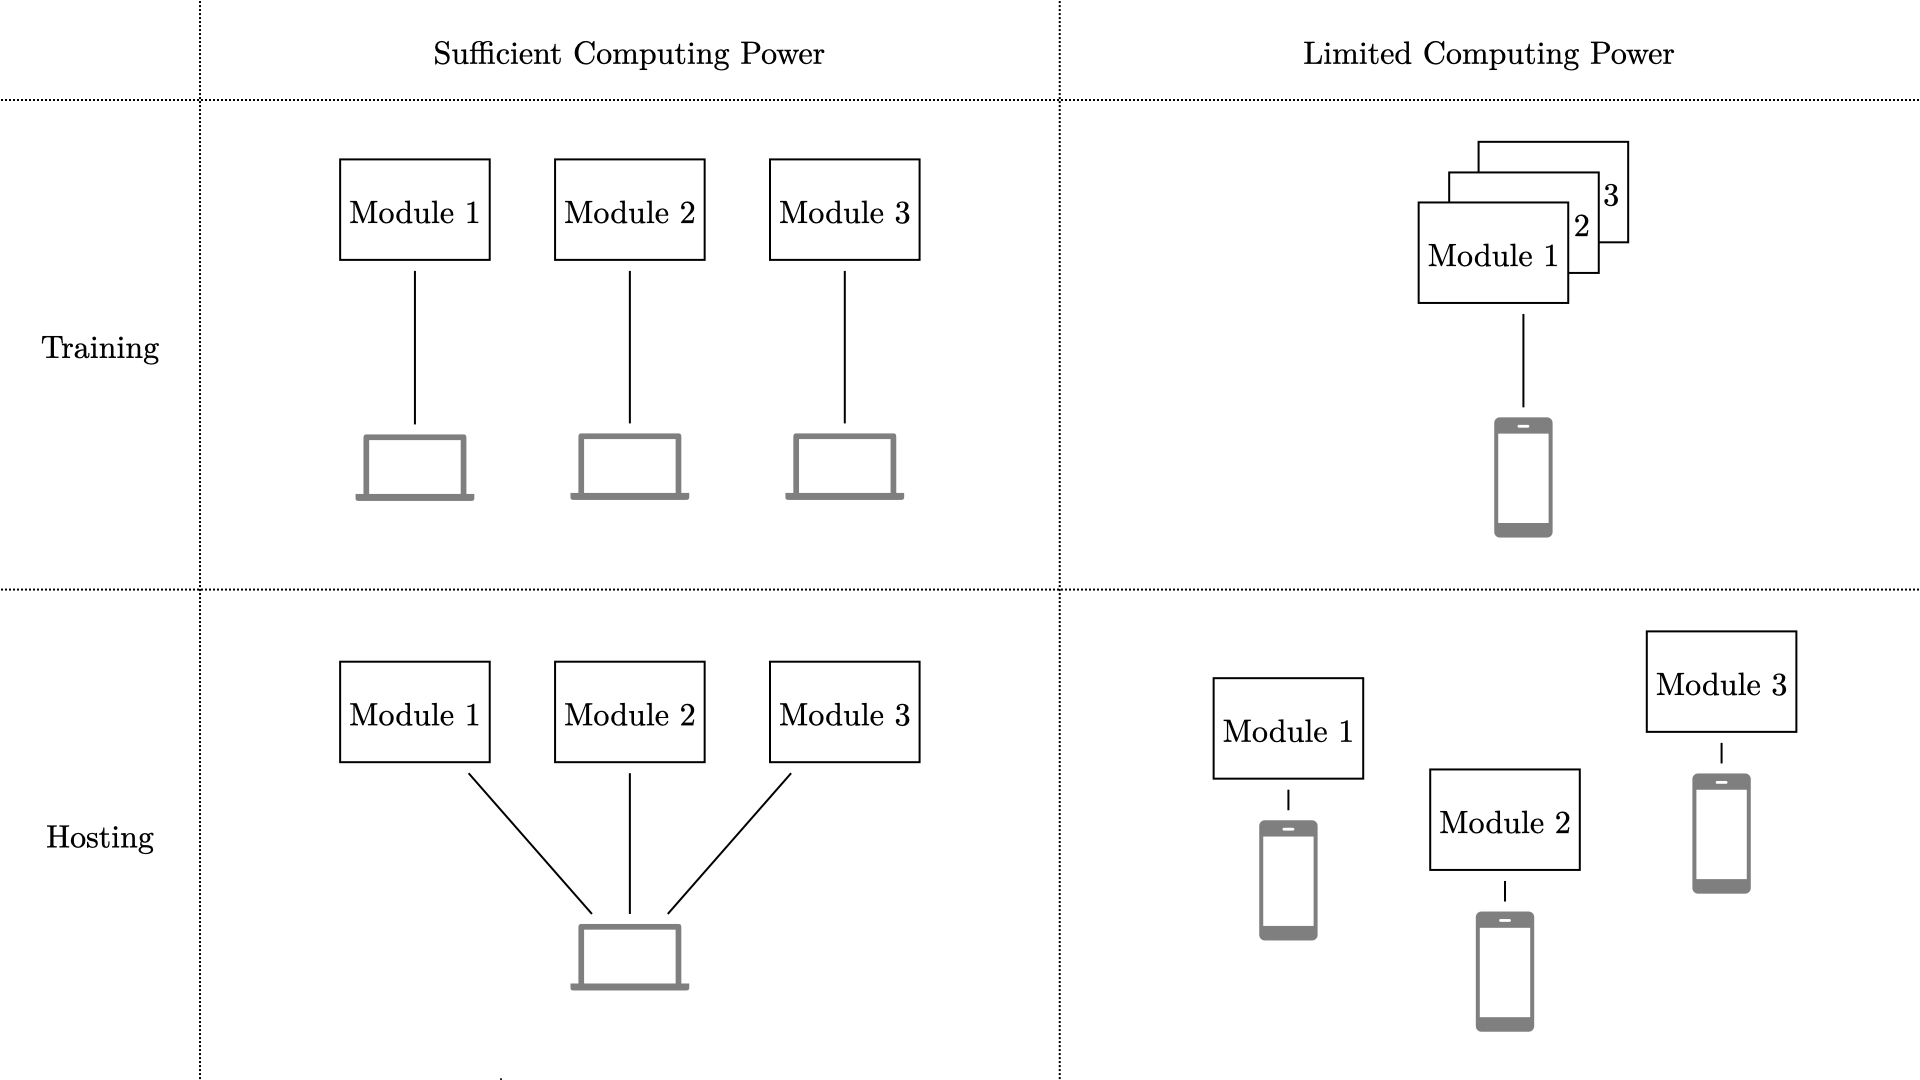
\includegraphics[width=\textwidth, trim=0 -25 0 -25, clip]{thesis/graphics/graphics/training_hosting.jpeg}
    \caption{A modularized architecture allows for flexible adaptation to the available hardware. With sufficient computing power, the individual submodules can be trained in parallel and hosted on the same physical entity. However, in scenarios with limited resources the modules can be trained serially at the expense of a higher overall training duration and, in scenarios such as IoT (Internet of Things) networks, also be hosted distributedly.}
    \label{fig:modularization_training_hosting}
\end{figure}        
        
        \begin{itemize}
            \item \textbf{Hardware constraints:} Decomposing models into smaller submodules facilitates accessibility of ML in hardware constrained environments. Consider a scenario with limited availability of computing power, e.\,g.\ for independent researchers, companies without access to a dedicated datacenter or local relearning on constrained devices such as smartphones. While it may not be possible to train a large network in such a situation due to memory restrictions, it might very well be possible to train multiple smaller sized ones one at a time.
            
            Secondly, in the case of large-scale, enterprise-size models, hardware restrictions may arise from the fact that the model becomes too big to be stored and executed on a single physical device. In such a scenario, decomposition makes the model inherently more accessible to distribution. E.\,g.\ each submodule could be hosted on a different physical or virtual device and be treated like a dedicated microservice.
            \item \textbf{Resource efficiency:} Modular networks have the advantage over conventional models that they allow for targeted assignment of computational resources. I.\,e., given a heuristic to estimate the influence of the individual submodules' performance on the overall performance of the network, it is possible to allocate additional resources to those areas where they yield the greatest improvement.
            
            Furthermore, neural networks as means of numeric approximation generally suffer from diminishing returns of additional DOFs (Degrees of Freedom) with increasing number of trainable parameters (cf.\ e.\,g.\ \cite{Lawrence1996-uj}). Simply put, adding another neuron to a small model tendentially reduces the absolute error by a larger margin than adding the same additional neuron to a larger model. Similarly, improving a large network by the same absolute error margin as a smaller network is computationally more expensive. Consequently it can be hypothesized that it is computationally more efficient to increase the size of $n$ submodules of a composed network by one parameter each in contrast to adding $n$ parameters to a comparable monolithic model instead.
        \end{itemize}
\end{itemize}

However, similar to conventional software systems, there are also disadvantages regarding the decomposition of ML models from an architectural point of view:

\begin{itemize}
    \item \textbf{Increased structural complexity:} The more components are involved in the overall behavior of an integrated system, the higher is the inherent structural complexity of that system. Above a certain degree, this hampers comprehensibility, impedes traceability and makes it more susceptible to errors. This effect equally applies to composed networks in comparison to their respective monolithic counterpart.
    \item \textbf{Reduced resilience:} Although not (necessarily) the case when all components of a composed network are hosted on the same physical or virtual platform, distributed systems generally suffer from reduced resilience due to effects such as inter-module package loss, stochastic latencies, concurrency and synchronization issues, etc. A comprehensive overview regarding the implications of distribution on software systems can be found in \cite{Lynch1989-ev} and \cite{Van_Steen2017-gb}.
    \item \textbf{Higher inference times:} Even though each individual module of a composed network is smaller than a comparative monolithic model, contemporary computer architecture, especially that of GPUs, is widely optimized for tensor multiplications. Hence, one-time operations such as loading a model take disproportionally more time than the calculation of the prediction itself. As a result, if one frequently switches between models as is the case in a modular network, this additional overhead induced by each submodule causes the overall model to be slower than its monolithic counterpart. Although this may not be of relevance for all applications, several scenarios certainly require short inference times.
\end{itemize}

\begin{figure}[bt]
    \centering
	    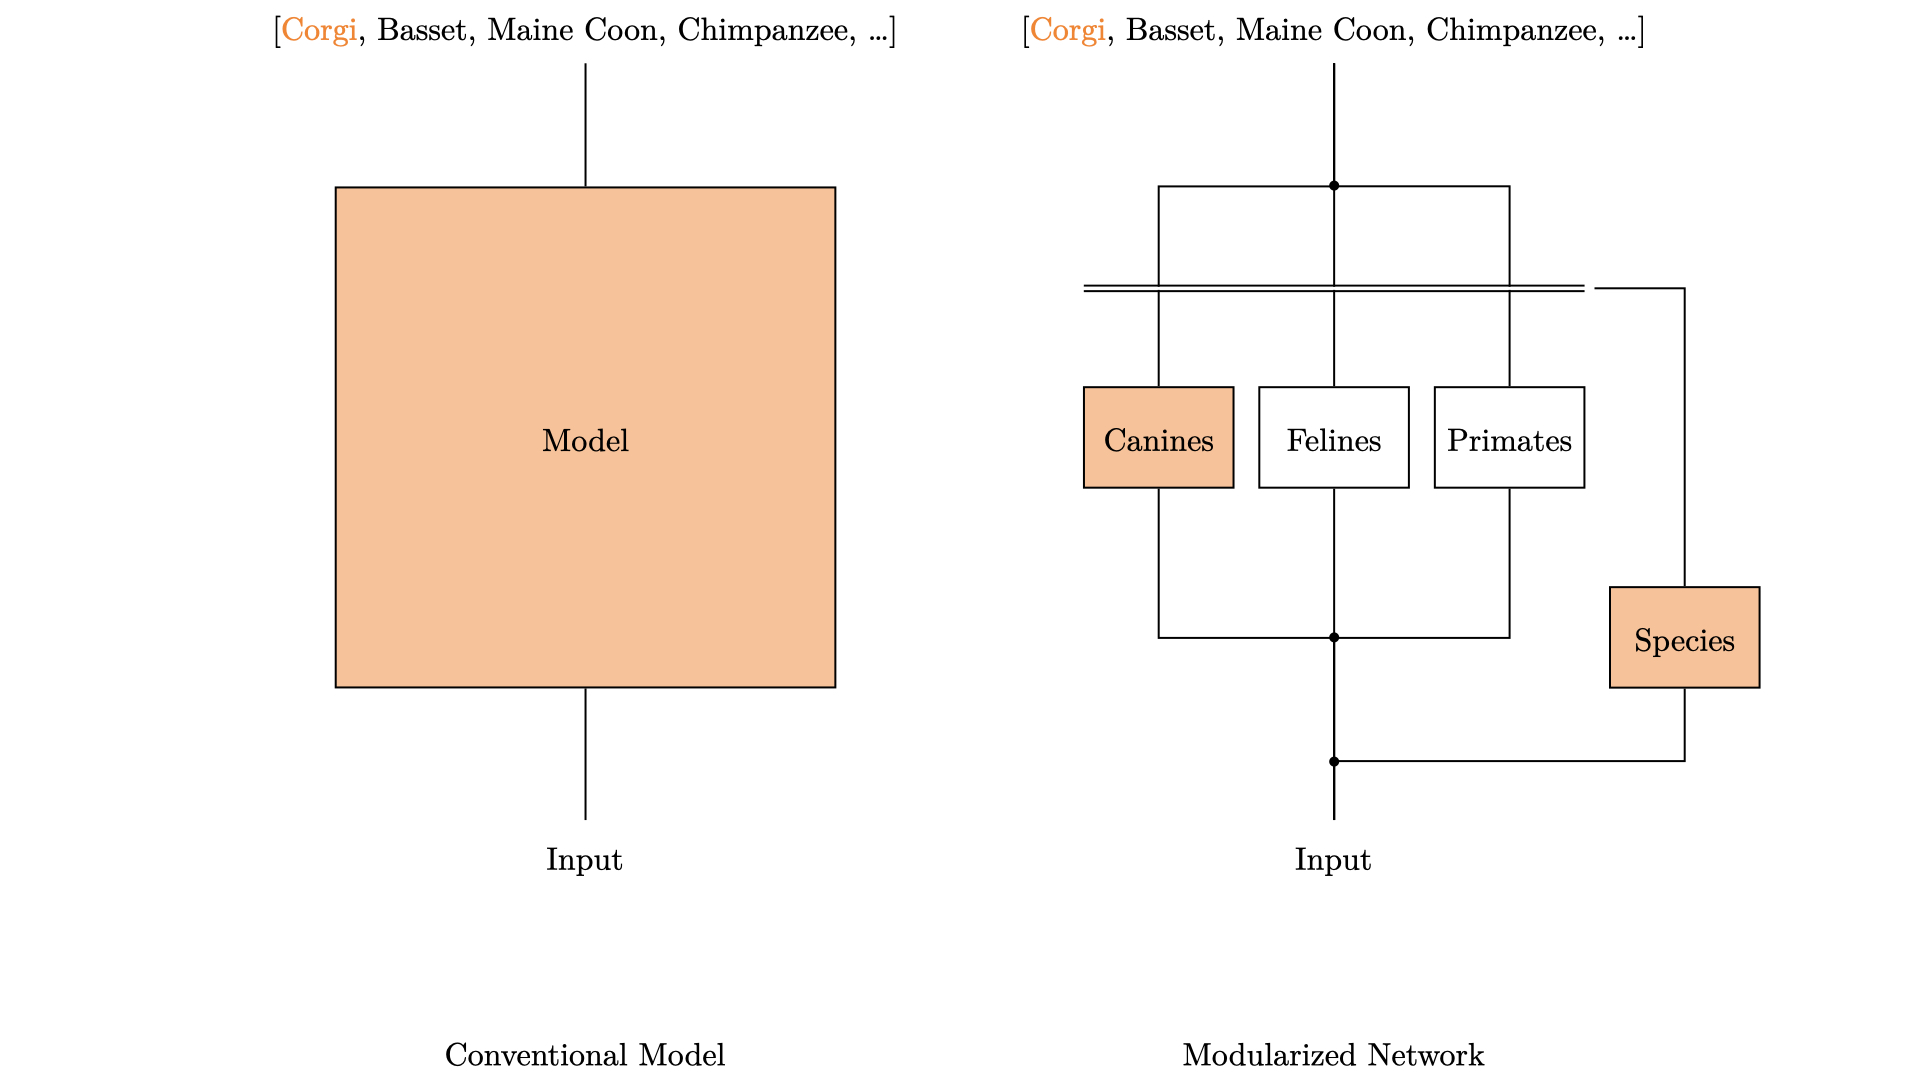
\includegraphics[width=\textwidth, trim=150 0 150 0, clip]{thesis/graphics/graphics/extensibility.jpeg}
    \caption{A modularized architecture increases the adaptability of once-trained models. By only having to retrain a small fraction of submodules when a change to the data base is made (in this example "Canines" and "Species"), retrainability and extensibility are facilitated.}
    \label{fig:modularization_extensibility}
\end{figure}

\textbf{ML motivated:} The former juxtaposition is mainly based on the software-nature of neural networks and thus not dissimilar to many other software systems for which the effects of modularization have already been extensively studied. However, also from a ML perspective, a modular structure possesses several desirable characteristics with regard to practical applicability. In the following, we again first consider advantages then disadvantages:

\begin{itemize}
    \item \textbf{Simplified retrainability:} In many applications, the data base underlying a model undergoes change over the course of the latter's lifecycle, e.\,g.\ new data of formerly underrepresented classes might become available or task-dependent properties such as seasonal changes in sales may induce distributional shift in subcategories. In these situations it is usually desirable to retrain the model to reflect these changes in the data base. While for a monolithic network this unavoidably affects the whole model, this is not necessarily the case for a composed network. To stick with the previous example, consider e.\,g.\ the scenario that new data of a formerly underrepresented class becomes available subsequent to the initial training. In this case, the concerned submodule associated with this particular class can easily be retrained while all other modules stay unaffected.
    \item \textbf{Extensibility:} Following the same basic idea, composed networks are more extensible than their monolithic counterpart. If e.\,g.\ a submodule on the final layer is to be extended by an additional category as depicted in figure \ref{fig:modularization_extensibility}, the change is locally restricted to that respective module. In general, only the affected submodule and all directly dependent modules have to be retrained.\footnote{This is similar to the previously discussed aspect of "Modifiability" motivated through the inherent software-nature of the model; as programmatic changes and retraining always go together for composed networks, the two different perspectives are hardly separable in this regard.}
    \item \textbf{Ability to build the model from pre-trained submodules:} One of the arguably greatest weaknesses of DL lies in the inefficiency to reuse once learned networks. In practice, models are commonly trained from scratch time and again for each new task. However, with composed networks it is possible to construct a model from individual, small-size building blocks that can easily be reused in other contexts (cf.\ e.\,g.\ figure \ref{fig:modularization_transferability}).
    
    To give a practical example, a manufacturer of sensory equipment such as LiDAR or laser measurement systems could provide a dedicated, bespoke and context-independent model for every sensor that outputs preprocessed information such as, in the case of LiDAR, shape and position of detected objects instead of raw sensory values. An application like an autonomous vehicle that integrates such components can then simply build on top of the manufacturer-provided modules for its own specific model. However, the very same sensors could also easily be deployed in very different scenarios without the need for adjustments.
    
    Another example would be a network whose submodules were trained to learn elementary functionalities each. One module might e.\,g.\ learn to filter out white noise from input data, another one might be responsible for edge detection, etc. It is now rather intuitive that these submodules can easily be reused in other scenarios as their scope is not limited to one specific application alone, comparable to how sometimes specific convolutional layers are refactored to speed up training of CNNs in practice.
    
\begin{figure}[tb]
    \centering
	    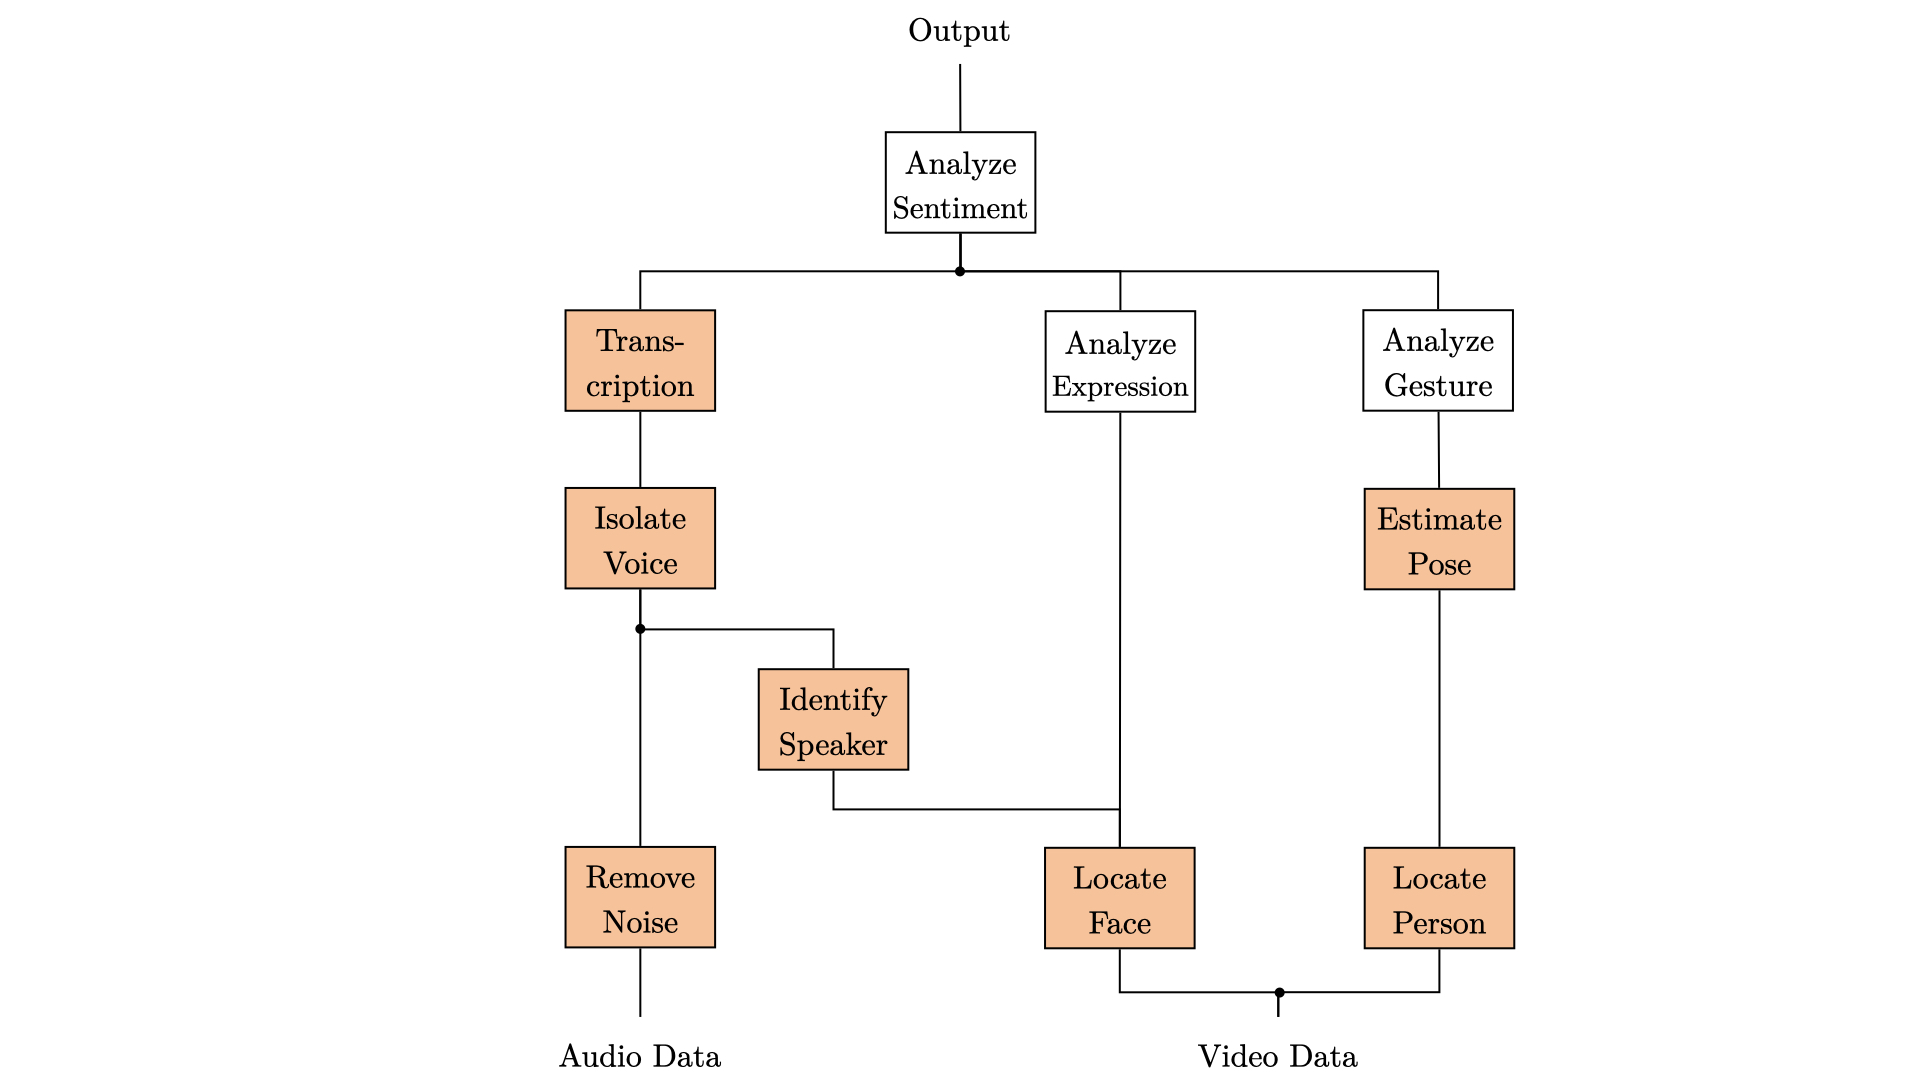
\includegraphics[width=\textwidth, trim=250 0 250 0, clip]{thesis/graphics/graphics/transferability.jpeg}
    \caption{Exemplary composed network for sentiment analysis. While the overall model is highly specialized, i.\,e.\ tailored to a specific task, the individual submodules constitute rather general functionalities and can easily be reused in other applications. In this illustrative example, generic building blocks (denoted in orange) could be used for seven out of ten modules.}
    \label{fig:modularization_transferability}
\end{figure}

    \item \textbf{Increased accessibility to transfer learning:} Similar to the previous point, since decomposing a model into different submodules reduces the specificity of the individual modules, modularization makes the overall network more accessible to transfer learning. The latter generally requires a reference model that is at least partly related to the target model to be applicable. It is easy to see that it is much simpler to find a fitting reference model for a module of rather elementary functionality than for a complex, task-specific expert model.
    \item \textbf{Increased interpretability:} A network composed from multiple submodules has the advantage of providing several breakpoints throughout the decision making process. It de facto breaks up the black box that is the respective monolithic counterpart and provides insights in how the final prediction is formed, thus facilitating comprehensibility of the model's behavior. We hypothesize that part of the reason for the above is that this kind of incremental reasoning is close to the human decision making process, similar to how we also naturally tend to break down complex problems in smaller, simpler ones.
    \item \textbf{Increased error traceability:} Another benefit of being able to trace the decision making process throughout the network through the interim results of the different submodules is that it facilitates traceability of errors and identification of error sources in general. I.\,e.\ by tracing the flow of information through the composed network, it is possible to identify not only why an error happens, but also where it occurs. While the former provides an understanding of the nature of the error, the latter indicates where exactly adjustments have to be made to fix this deficit.

\begin{figure}[b!]
    \centering
	    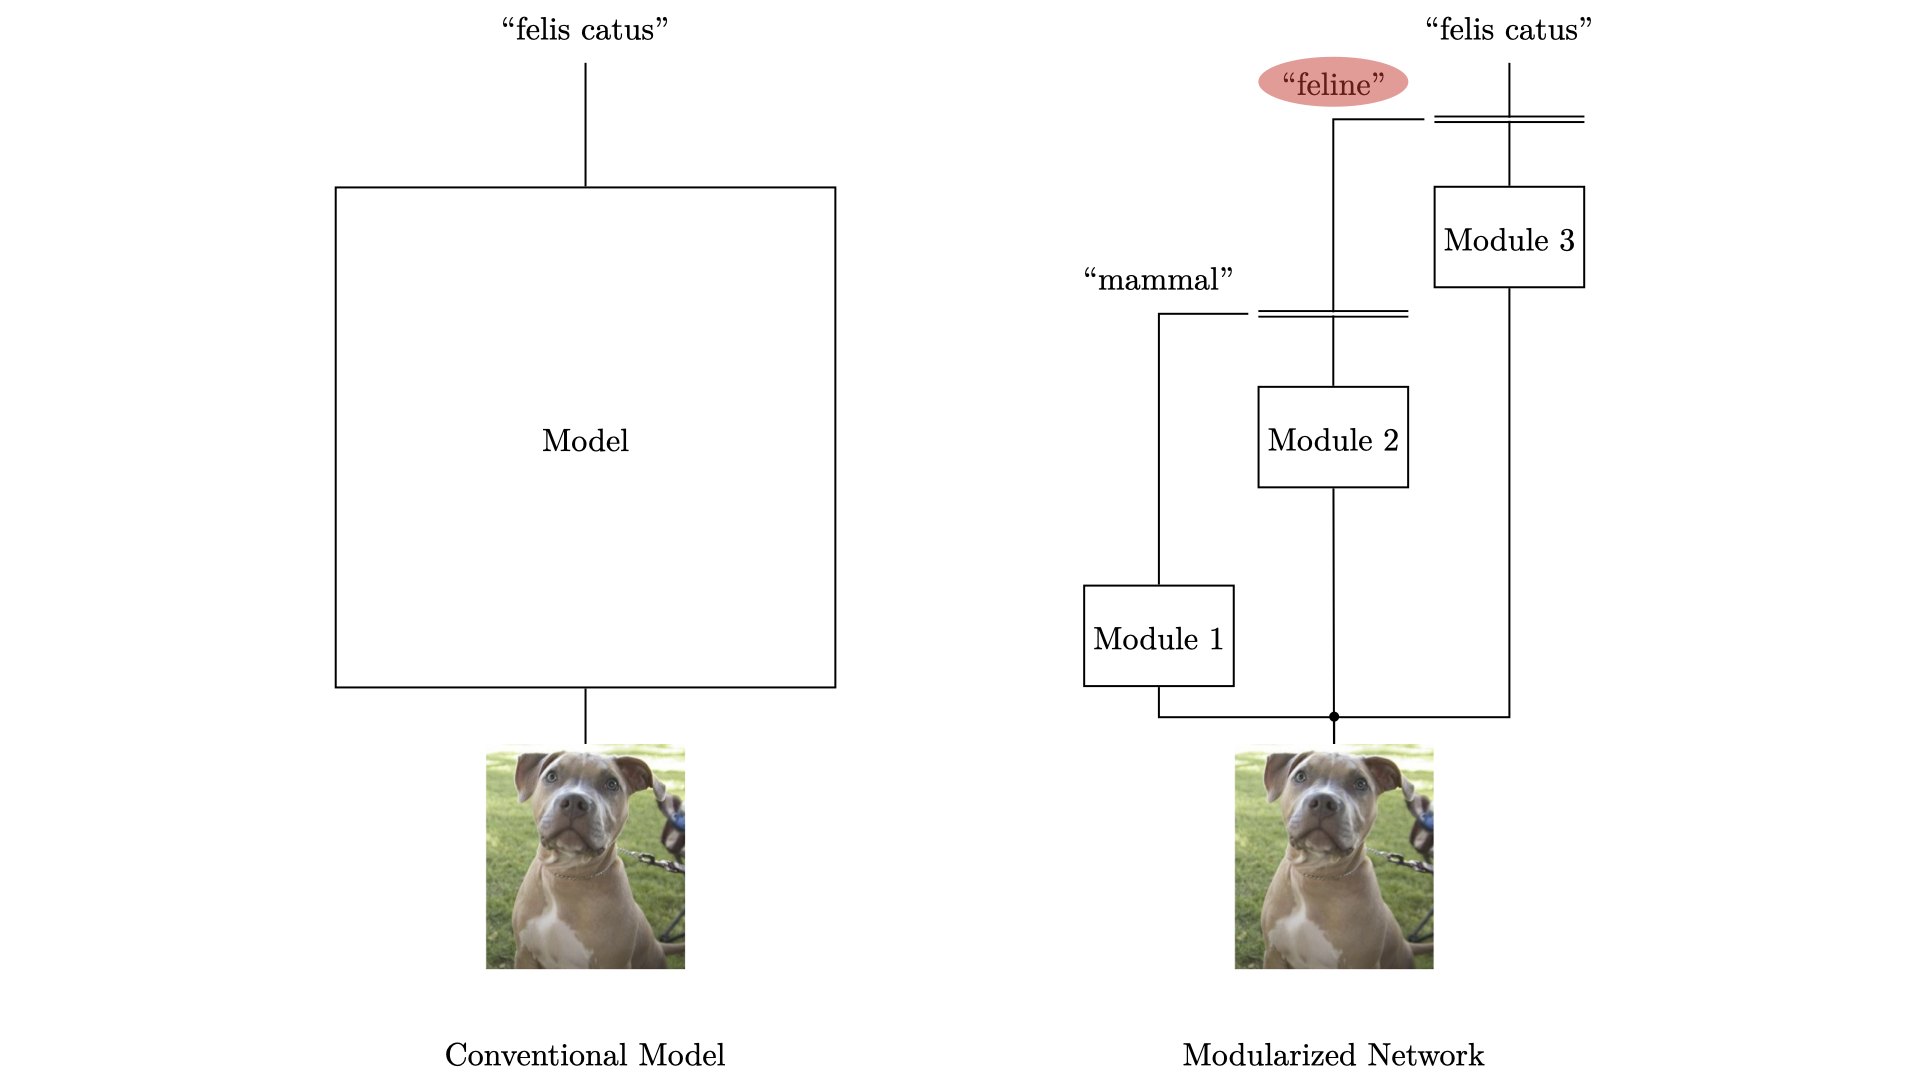
\includegraphics[width=\textwidth, trim=250 0 250 -50, clip]{thesis/graphics/graphics/error_traceability.jpeg}
    \caption{In the case of a conventional model, it is hardly possible to pinpoint the exact reason for faulty predictions on an individual basis. However, in the case of the composed network it is easy to see that the error is caused by the second submodule.}
    \label{fig:modularization_error_traceability}
\end{figure}
    
    Consider for instance a network for image recognition in which one upstream submodule constantly categorizes dogs as cats, thus flawing the final prediction whenever an image of a dog is input into the model as depicted in figure \ref{fig:modularization_error_traceability}. With this information it is easy to see that, to correct this error, it is necessary to e.\,g.\ retrain the respective dog-cat-submodule with additional images of dogs.
    \item \textbf{Reduction of individual model size:} Smaller model size is attractive in practical applications as it disproportionally reduces the development effort for the individual modules. Not only are smaller models easier to optimize as they usually have less hyperparameters; they also train and converge much faster than large networks since they possess fewer trainable weights and need less data, thus accelerating the feedback loop, i.\,e.\ the time needed before the developer receives a feedback on the model's performance after making a change.
    \item \textbf{Structural flexibility:} Composing a model from multiple independent submodules greatly increases its structural flexibility. This entails various beneficial effects regarding practical applicability:
        \begin{itemize}
            \item \textbf{Possibility to tune different submodules individually:} As the submodules of a composed network are independent of each other, they can be tuned individually regarding basic architecture and hyperparameters. This allows for adaptation of the modules to their respective sub-domains and extensive optimization during training.
            \item \textbf{Possibility to employ different model types for different submodules:} While in this work we only consider neural networks as submodules for composed models, it is theoretically possible to employ different kinds of ML models to better match the nature of the different inputs. If e.\,g.\ one modality is inherently highly clusterable, one may decide to employ k-NN (k-Nearest Neighbour) for that specific module to match this property.
            \item \textbf{Possibility for additional error correction mechanisms within the model at different hierarchy levels:} In many practical applications it is important to be able to recognize errors and detect faulty decisions as early as possible and react to them. In composed networks it is possible to place additional detection and correction mechanisms in between submodules to recognize and possibly recover from errors early on during the decision process before they propagate through the whole system.
            
            Consider e.\,g.\ a decision making model for an autonomous vehicle. In the first forward-pass, the obstacle detection submodule reports an object in the direct trajectory of the car. Due to a fatal sensory error, however, in the second forward-pass, no obstacle is reported at all. A human decision maker would intuitively know that breaking would be the appropriate action in case of uncertainty in this situation. A (naive) ML model on the other hand might decide that, since the obstacle seems to be gone, it is okay to keep driving instead. To avoid such situations, an additional module to check the consistency of consecutive predictions could be placed after the obstacle detection in a composed network.
            \item \textbf{Possibility to combine ML models with deterministic software components:} Generally, composed networks provide the possibility to construct models from a combination of ML and deterministic software components, thus e.\,g.\ enabling the creation of fallback routines at different hierarchy levels. A submodule could hence for instance be trained to output the control variable for a process in combination with a confidence with regard to the predicted value. In case the confidence is below a certain threshold, i.\,e.\ the module is unsure about its prediction, the system could then switch to a conventional deterministic plant as a fallback (cf.\ e.\,g.\ figure \ref{fig:modularization_structural_flexibility}).
            
\begin{figure}[tb]
    \centering
	    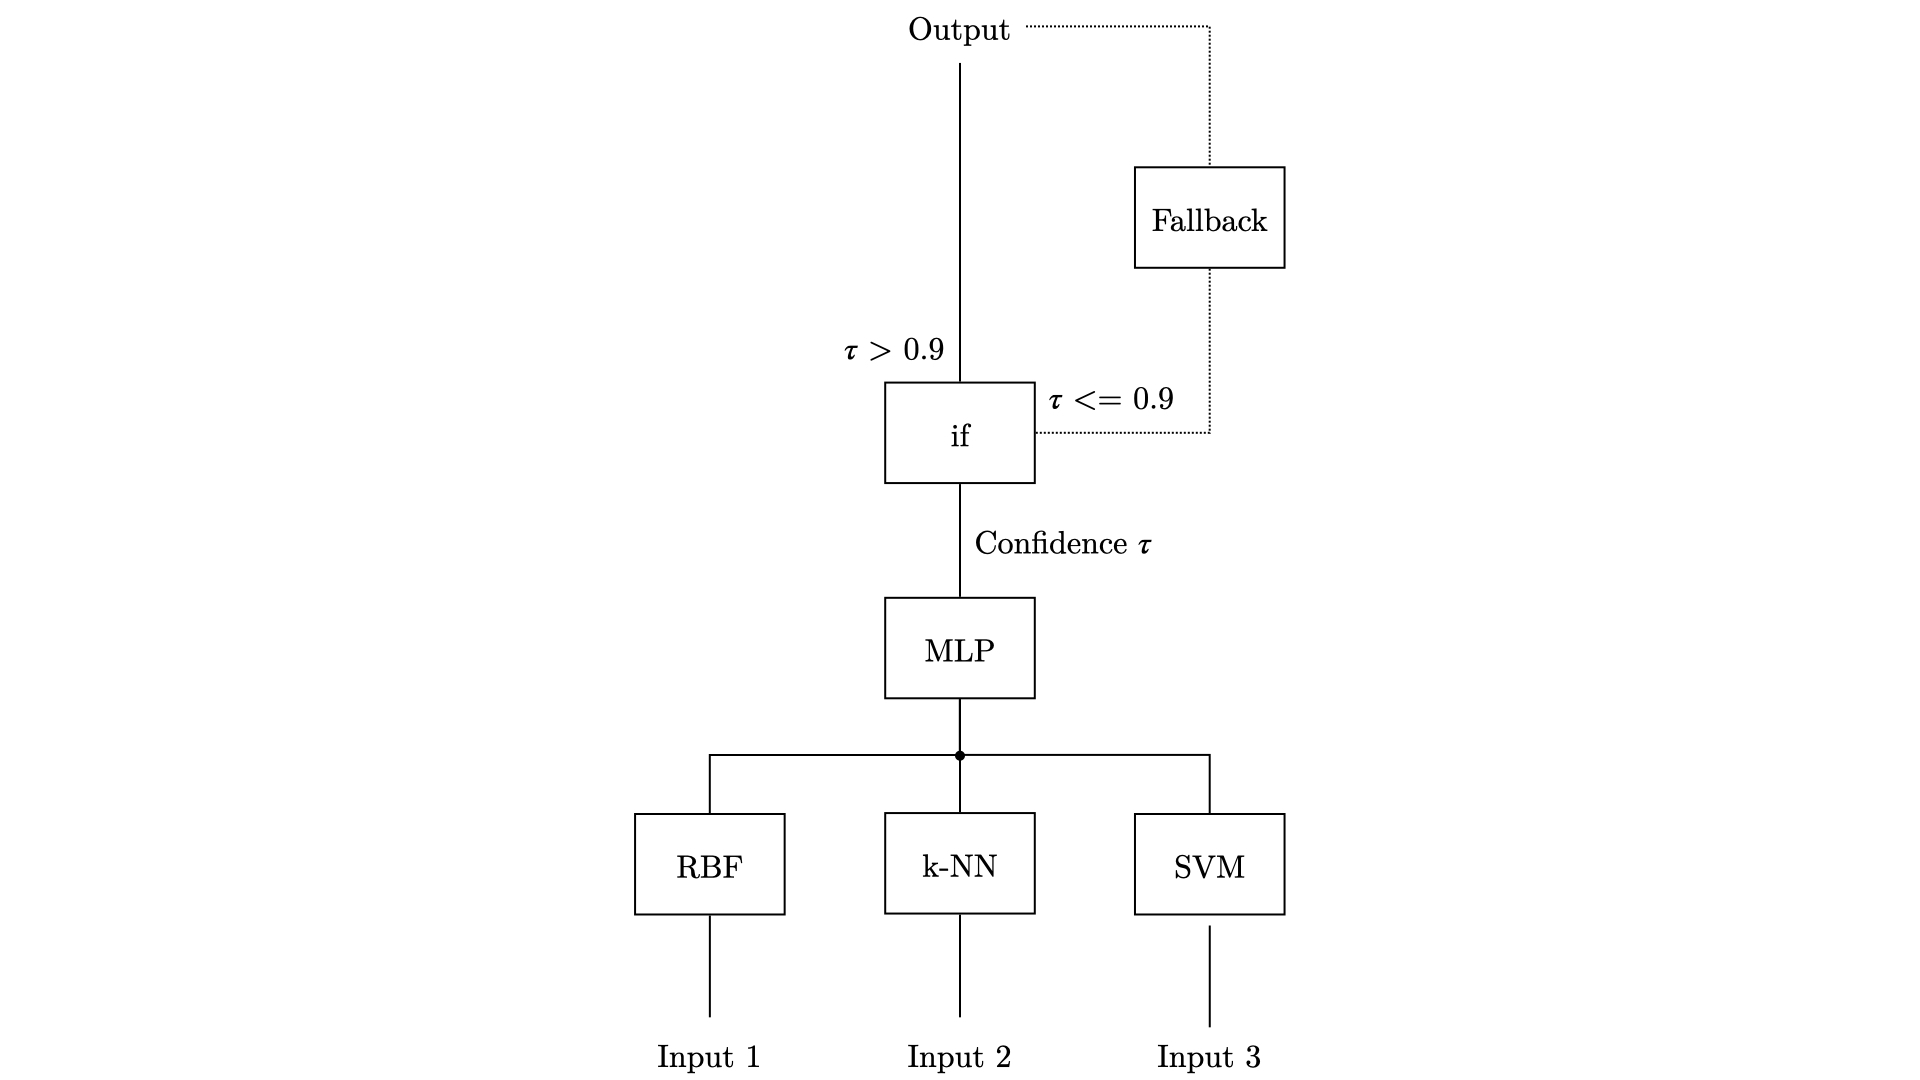
\includegraphics[width=\textwidth, trim=250 0 250 0, clip]{thesis/graphics/graphics/structural_flexibility.jpeg}
    \caption{Composing models from submodules increases the architectural flexibility and enables the combination with deterministic software components.}
    \label{fig:modularization_structural_flexibility}
\end{figure}        
            
            Another advantage of this is the possibility to define actions at early stages of the model analogous to reflexes. Consider e.\,g.\ the above example of obstacle detection in autonomous driving. If an object does suddenly appear in front of the car (e.\,g.\ a kid running out between parked vehicles), the obstacle detection module could directly trigger an emergency break for an instantaneous action without the information having to traverse through the rest of the model first, thus reducing reaction times.
        \end{itemize}
    \item \textbf{Accelerated learning through pre-definition of coherent sub-structures:} By inferring knowledge about the structure of the transformation to be learned into the model through manual definition of submodules, the necessity for the model to learn these decompositions itself is removed. In its simplest form, i.\,e.\ as long as solely neural networks are considered for submodules, this can be seen as equivalent to careful manual weight initialization in monolithic models\footnote{Consider a monolithic model for which parameter values are carefully chosen to create sparsely interconnected clusters of non-zero weights divided by regions of weights set to zero. The result is equivalent to a composed network.}. As a result the time necessary for the training of the model is shortened.
    
    In other words, by providing the model with information concerning the nature of the underlying task, learning is accelerated as the amount it has to learn is reduced. In this, modularization is in line with other approaches for knowledge inference such as ResNet \cite{He2015-cq}.
\end{itemize}

In contrast, the adverse effects introduced by modular model structure can be summarized as follows:

\begin{itemize}
    \item \textbf{Introduction of modularization errors:} Decomposing a monolithic network into individual submodules inevitably introduces additional error terms that negatively affect the model's performance. Simply put, by modulating the search space of the model, decomposition entails the risk of the latter losing the ability to model certain interrelations in the data similar to overly-aggressive pruning in neural networks. While removing the "right" connections allows the model to make more efficient use of its modeling capacity and speeds up the learning process, removing "wrong" ones, e.\,g.\ through naive decomposition, results in a non-compensable error.
    
    This aspect is a major adversary effect of modularization and does as such require special attention; it is therefore further elaborated in a dedicated discussion in section \ref{sec:compnet_error}.
    \item \textbf{Increased development overhead:} Even in the most trivial scenario where all submodules of a composed network are trained independently, each module has to be monitored and possibly tuned individually to avoid adverse effects such as overfitting. The same holds true for testing as well. Furthermore, additional preprocessing steps are likely to arise due to the necessity to e.\,g.\ adapt the labeling structure of the data base to the different hierarchy levels of the model or to divide the former into subsets for the individual modules. While these measures do not negatively impact the model performance, they do increase the development overhead before the network is operational.
\end{itemize}

Concluding, modular networks offer various benefits over conventional monolithic models. Noteworthily, however, the primary advantage consists in an increased practical applicability. In fact, as is argued in section \ref{sec:compnet_modularization_convergence_performance}, the possible performance gain from modularization is virtually negligible in practice. As such, our approach can be said to be orthogonal to conventional, performance-oriented approaches. Nevertheless, we consider modularization to be a technique worth researching in more detail as it does not only address several of the inherent shortcomings of DL, but also possesses various properties that are desirable in many practical applications. Therefore, with this work, we aim to provide a first theoretical and experimental basis regarding the implications of modularization on different aspects of model behavior and to inspire further research.

\cleardoublepage

\section{Composition of Meta-Networks from multiple Submodules%
         \label{sec:compnet}}

In this chapter, a theoretical foundation regarding the basic concept of modularization in a ML specific context shall be established. For that, different general dimensions constituting arbitrary ML models are identified. It is then examined how modularization can be applied to each of them and how it impacts the resulting model. Qualitative convergence and performance properties of composed networks are discussed. Secondly, the two primary variants of modularization are compared. Examples of combinatorial methods for each are given. The chapter is concluded by a discussion on the concept of modularization errors and a subsequent investigation of error propagation in different kinds of model compositions.

\subsection{Modularization of ML Models%
            \label{sec:compnet_modularization}}

Consider an arbitrary ML model. While seeming like a single, cohesive system on the surface, it is in reality constituted from multiple different dimensions characterizing the concrete instantiation of the model:
            
\begin{itemize}
    \item \textbf{Task:} A task is an algorithmic description of a particular process relating a specific input to a specific output that can be expressed by means of mathematical or natural language statements. Every particular model instantiation is coupled to a specific, existence-giving task. It is the purpose of the model to learn the transformation defined by the latter.
    \item \textbf{Model:} Model in this case refers to the functional depiction of the pivotal task as well as all related sub-tasks. This includes aspects such as the concrete type and architecture of the employed model, preprocessing routines, training and testing procedures, etc.
    \item \textbf{Implementation:} Ultimately, every model is a piece of software. It can be interpreted as a projection of the functional model to the computational level. While not inferring any information on its own, the implementation very well affects the overall system in aspects such as (computational) performance, modifiability, etc.
\end{itemize}          
            
Now, contrary to the intuitive thought, modularization as a technique is not necessarily restricted to the architectural component of ML models. It is, instead, applicable to any of the aforementioned dimensions and yields different effects depending on the context (cf.\ e.\,g.\ figure \ref{fig:compnet_modularization_modularization_domains}).

For instance, the modeled task can be separated into several sub-tasks based on its inherent nature, that is, if it can be interpreted as a meta-task composed of multiple smaller tasks. Consider e.\,g.\ a system to digitize handwritten texts. In this scenario, the meta-task could e.\,g.\ be broken down into three independent sub-tasks, each with much smaller scope -- one module to recognize individual characters, a subsequent module to concatenate letters to words and a third one for spell checking.

The model layer directly reflects such decompositions on the task layer. However, within these constraints, modularization can occur independent of the considered process as well, e.\,g.\ motivated by the inherent structure of the underlying data base. If the domain is e.\,g.\ well clusterable, one might for instance decide to employ a mixture of spatial models such as RBFs (Radial Basis Functions).

Both modularization on the task as well as on the model layer infer information augmenting the topology of the search space into the model. We denote this as auxiliary information in contrast to primary information, i.\,e.\ knowledge contained in the relation between domain and codomain. Specifically, modularization enhances the structure of the search space by introducing additional constraints, effectively dividing it into several sparsely connected subspaces, each of which is of lower complexity than the composed space. The amount of auxiliary information inferred by a particular decomposition is proportional to the amount as well as the strictness (i.\,e.\ holonomic or non-holonomic) of the introduced constraints. Consequently, the existing modeling capacity can be utilized more efficiently as the amount of information the model has to learn explicitly is reduced.

The increased specificity of the model, however, results in a reduction of the generalizability at the same time as described by the "No Free Lunch" theorem by \cite{Wolpert1997-fu}. Hence modularization is always case specific and can hardly be transferred between tasks. I.\,e.\, while the submodules can easily be reused in other applications, the individual decomposition has to be conceived anew for each new model.

The software layer on the other hand does not infer any information into the system. It can thus be designed in an arbitrarily modularized way as long as the projection of the functional model is retained. As mentioned before, this may still impact aspects such as modifiability or computational performance.

\begin{figure}[tb]
    \centering
	    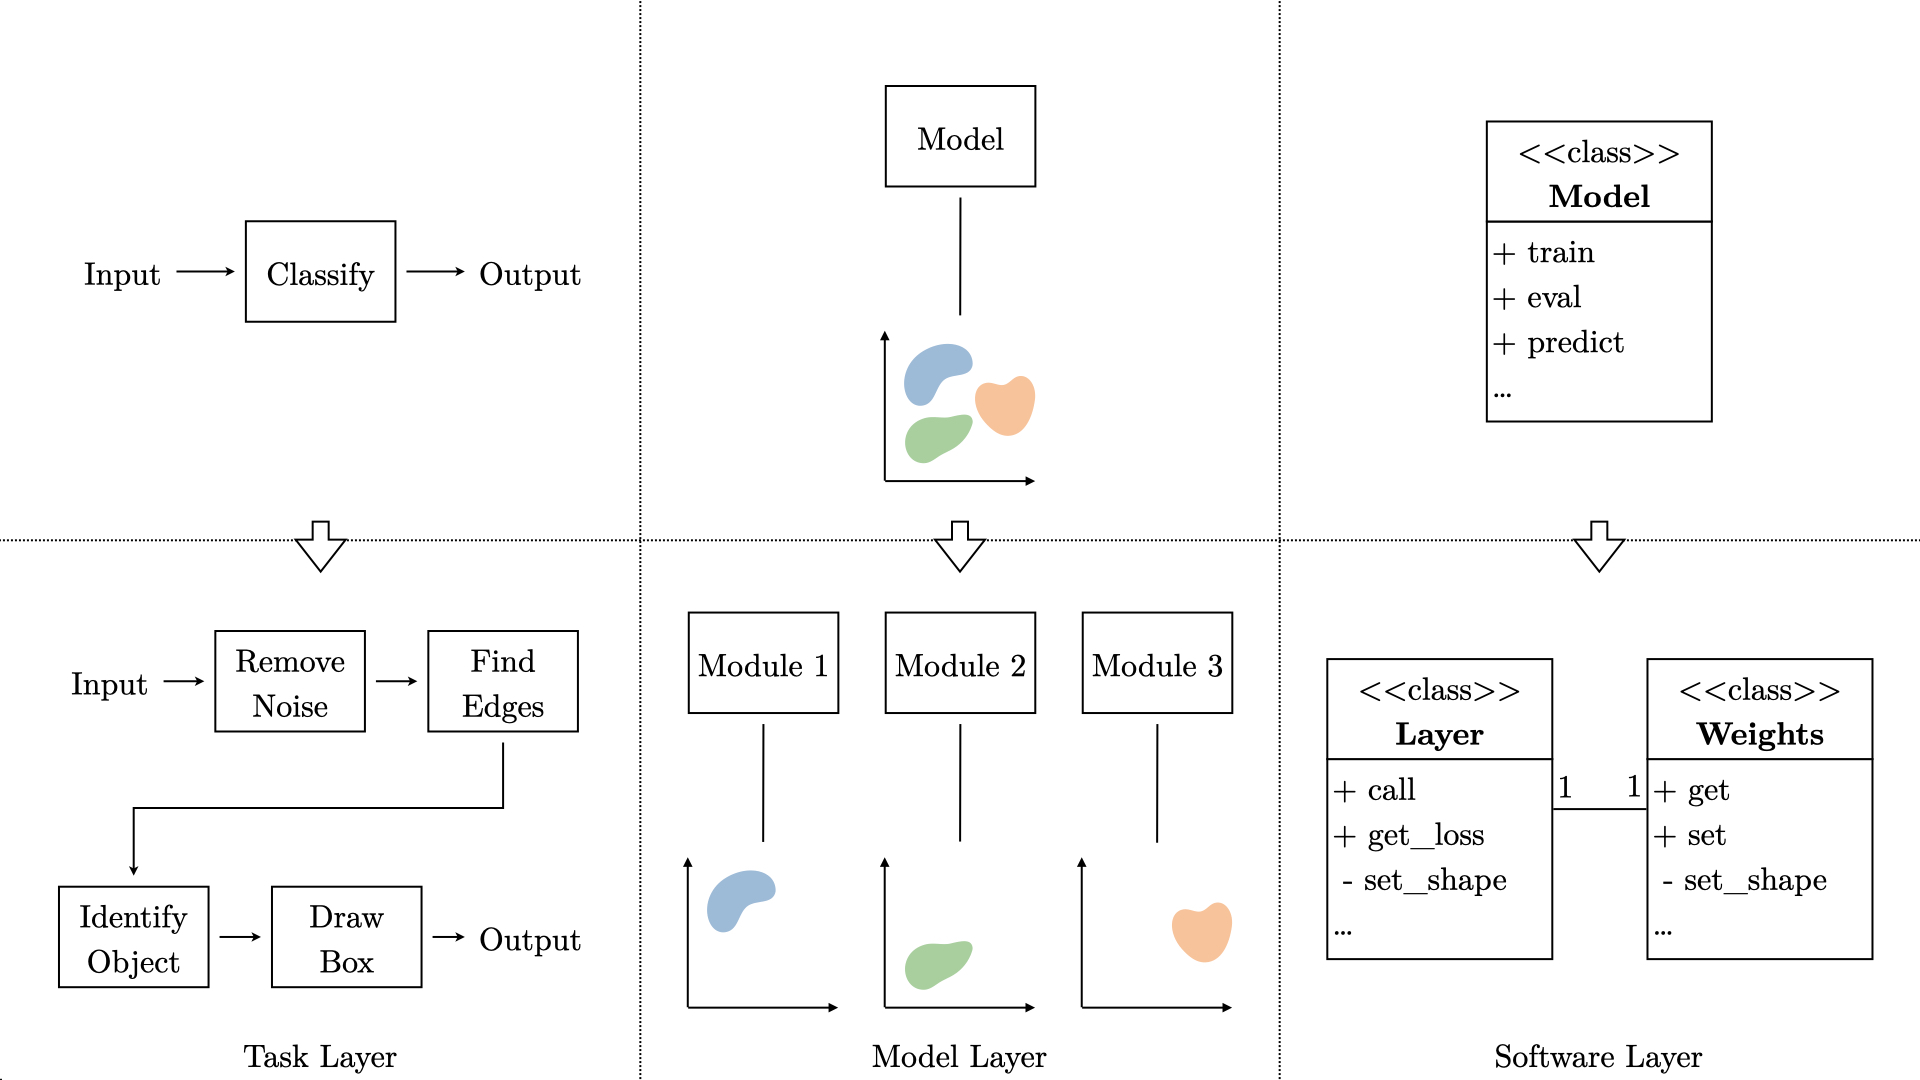
\includegraphics[width=\textwidth, trim=0 -25 0 -25, clip]{thesis/graphics/graphics/modularization_domains.jpeg}
    \caption{Modularization can be applied to any of the three domains constituting a specific model instantiation.}
    \label{fig:compnet_modularization_modularization_domains}
\end{figure}

\subsection{Convergence and Performance Properties of Composite Models%
            \label{sec:compnet_modularization_convergence_performance}}
            
An interesting and certainly legitimate question in regard to composed networks is whether, just because convergence was guaranteed for a given model before modularization, this property is retained after decomposition as well. Alas, answering this is beyond the scope of this work. Here, we solely focus on the opposite directionality.

\newtheorem{theorem}{Theorem}
\begin{theorem}
    Consider a network composed from multiple submodules. If all individual modules of this network converge, the overall model converges as well.
\end{theorem}

Intuitively, the meta-search space of the overall model is the superposition of the individual modules' sub-search spaces. Similarly, the optimum in the composite space is formed by superimposing the optima of the subspaces. Obviously, as long as all submodules converge against their respective optima, the overall model equally converges. If all subspaces are disjoint, the resulting meta-optimum is a point; otherwise it consists of a higher dimensional region.

Note, however, that the optimum found this way is not necessarily the global optimum of the meta-space. The problem of finding a decomposition that guarantees the latter is strongly related to the question posed at the beginning of this section and as such equally beyond the scope of this work.

Conversely, convergence within the individual submodules can be understood as convergence in the meta-space along the dimensions of the respective subspace against the projection of the meta-optimum to this subspace. This is comparable to freezing all DOFs of the meta-space except for the ones of a specific submodule and solely performing optimization, e.\,g.\ via SGD (Stochastic Gradient Descent), on the remainder. Albeit the fineness of the descent consequently decreases, the convergence properties remain unaffected.

As an additional observation, the maximum improvement of performance a composed network can achieve over a comparative monolithic model is limited to the amount of information immanent to the modularization. If the modularization does not add any auxiliary information to the model, the original search space is retained and the global optimum remains the same in consequence as well. More specific decompositions infer more prior knowledge and hence the higher the theoretically possible performance gain; the model becomes more susceptible to modularization error at the same time, however (cf.\ section \ref{sec:compnet_error}).

Albeit, since neural networks are universal approximators as proven by \cite{Kolmogorov1957-ok} and \cite{Hornik1989-nf}, there exists no possible decomposition that the original monolithic model could not have learned itself given enough time and resources. Hence, a relative improvement of performance through modularization in comparison to a given monolithic model can only be achieved as long as the latter is not over-parameterized; otherwise, a decomposition of equal modeling capacity can at best reach, but not exceed the performance of the original network.

Consequently, the performance gain is virtually negligible; the primary advantage of this approach consists in the positive impact on practical applicability as described in section \ref{sec:motivation}.

\subsection{Types of Modularization%
            \label{sec:compnet_modularization_types}}

There are two fundamental ways to decompose a system into submodules, horizontal and vertical decomposition. Note that with "system", we denote any structure or process that transforms an arbitrary input into an equally arbitrary output here. Both types of modularization act on the transformation from domain to codomain and are not mutually exclusive, i.\,e.\ they are freely combinable.

\textbf{Horizontal Modularization:} Horizontal modularization describes the process of decomposing an arbitrary process in a suitable way to approximate a parental process through multiple parallel (optimally independent) sub-processes. From a mathematical point of view, the decomposition can be understood as an optimization problem where a transformation from a certain domain to a codomain is to be separated in a way that the informational loss in comparison to the original transformation is to be minimized. For an optimal decomposition, the resulting modules are capable of modelling the primary information in its entirety; the auxiliary information inherently increases due to the additional holonomic constraints inferred by the separation into individual submodules. In consequence, the resulting meta-network learns faster but not necessarily better. Three forms of horizontal modularization are possible:

\begin{itemize}
    \item Decomposition in the domain with unchanged codomain and reconstruction of the original transformation via aggregation of the results of the different submodules
    \item Decomposition in the codomain with unchanged domain and reconstruction of the original transformation via merging / superimposing of the subspaces of the different submodules
    \item Arbitrary combinations of the former two
\end{itemize}

Common examples of techniques to aggregate / combine the results of the individual submodules include (cf.\ figure \ref{fig:compnet_modularization_types_horizontal_decomposition}):

\begin{itemize}
    \item Linear Opinion Pool (weighted addition of individual results)
    \item Multiplicative Opinion Pool (weighted multiplication of individual results)
\end{itemize}

The latter, however, is rarely used in practice due to its unfavorable qualities with regard to error propagation. More common is its variation, the Logistic Opinion Pool, i.\,e.\ addition of the logarithm of the individual results, especially if the submodules output probabilities (cf.\ e.\,g.\ \cite{Benediktsson1992-bl}). Appropriate weights can be found using various different methods ranging from simple averaging to Bayesian techniques (\cite{Xu1992-hp}).

\begin{figure}[htb]
    \centering
	    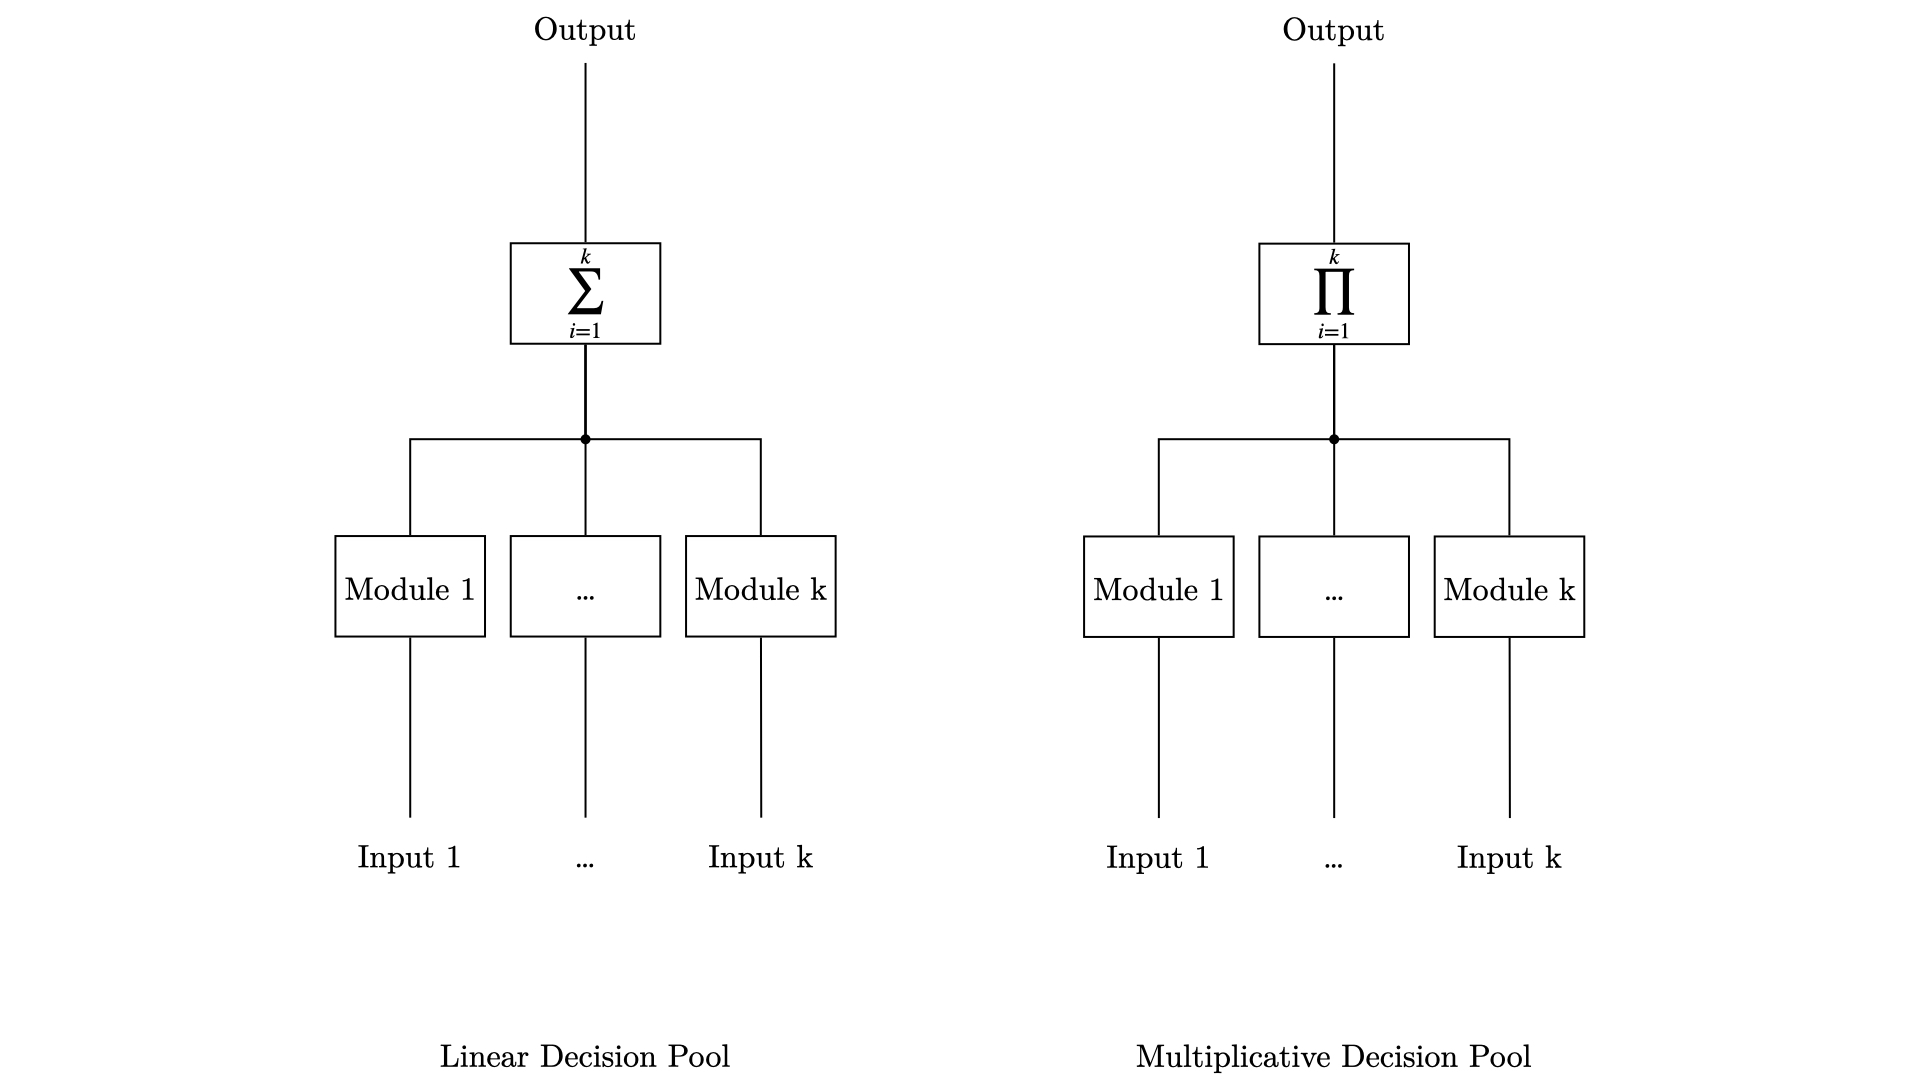
\includegraphics[width=\textwidth, trim=150 0 150 0, clip]{thesis/graphics/graphics/horizontal_decomposition.jpeg}
    \caption{Common variants of horizontal decomposition.}
    \label{fig:compnet_modularization_types_horizontal_decomposition}
\end{figure}

\textbf{Vertical Modularization:} Vertical modularization, also known as Layering, describes the process of modulating the information channel along which the primary information in the domain is mapped to the codomain by decomposing a process into different sub-processes, also called Layers, along the axis of transformation. The amount of primary information in the system is restricted by the maximum amount the informationally most limited layer can store. In other words, if e.\,g.\ any of the intermediate layers in a modular system possesses a single Boolean as sole output, it is impossible for outputs of subsequent layers (and thus the overall model) to be of higher complexity without additional input. Note, however, that the amount of primary information a layer can contain is composed of the cardinality as well as the interrelations of the states within the layer. Thus a pure dimensionality reduction from one layer to the next does not necessarily imply loss of information. Similar to horizontal modularization, vertical modularization increases the auxiliary information and hence the specificity of the system.

Examples of methods to connect subsequent layers include (cf.\ figure \ref{fig:compnet_modularization_types_vertical_decomposition}):

\begin{itemize}
    \item Chaining (the output of the first layer is used as the input of the second layer)
    \item Gating (the output of the first layer is used to modulate the informational flow in the second layer)
\end{itemize}

Popular applications leveraging vertical modularization e.\,g.\ include contemporary NLP (Natural Language Processing) architectures that chain neural networks and autoencoders.

As has been mentioned before, it is furthermore possible to combine horizontal and vertical decomposition in the same system. In this case, it is theoretically possible for primary information that has initially been lost through suboptimal horizontal decomposition (cf.\ following section) to be "restored" by employing a form of combinatorial mechanism at a higher layer, effectively recreating the original correlation between the different sub-domains.

\begin{figure}[htb]
    \centering
	    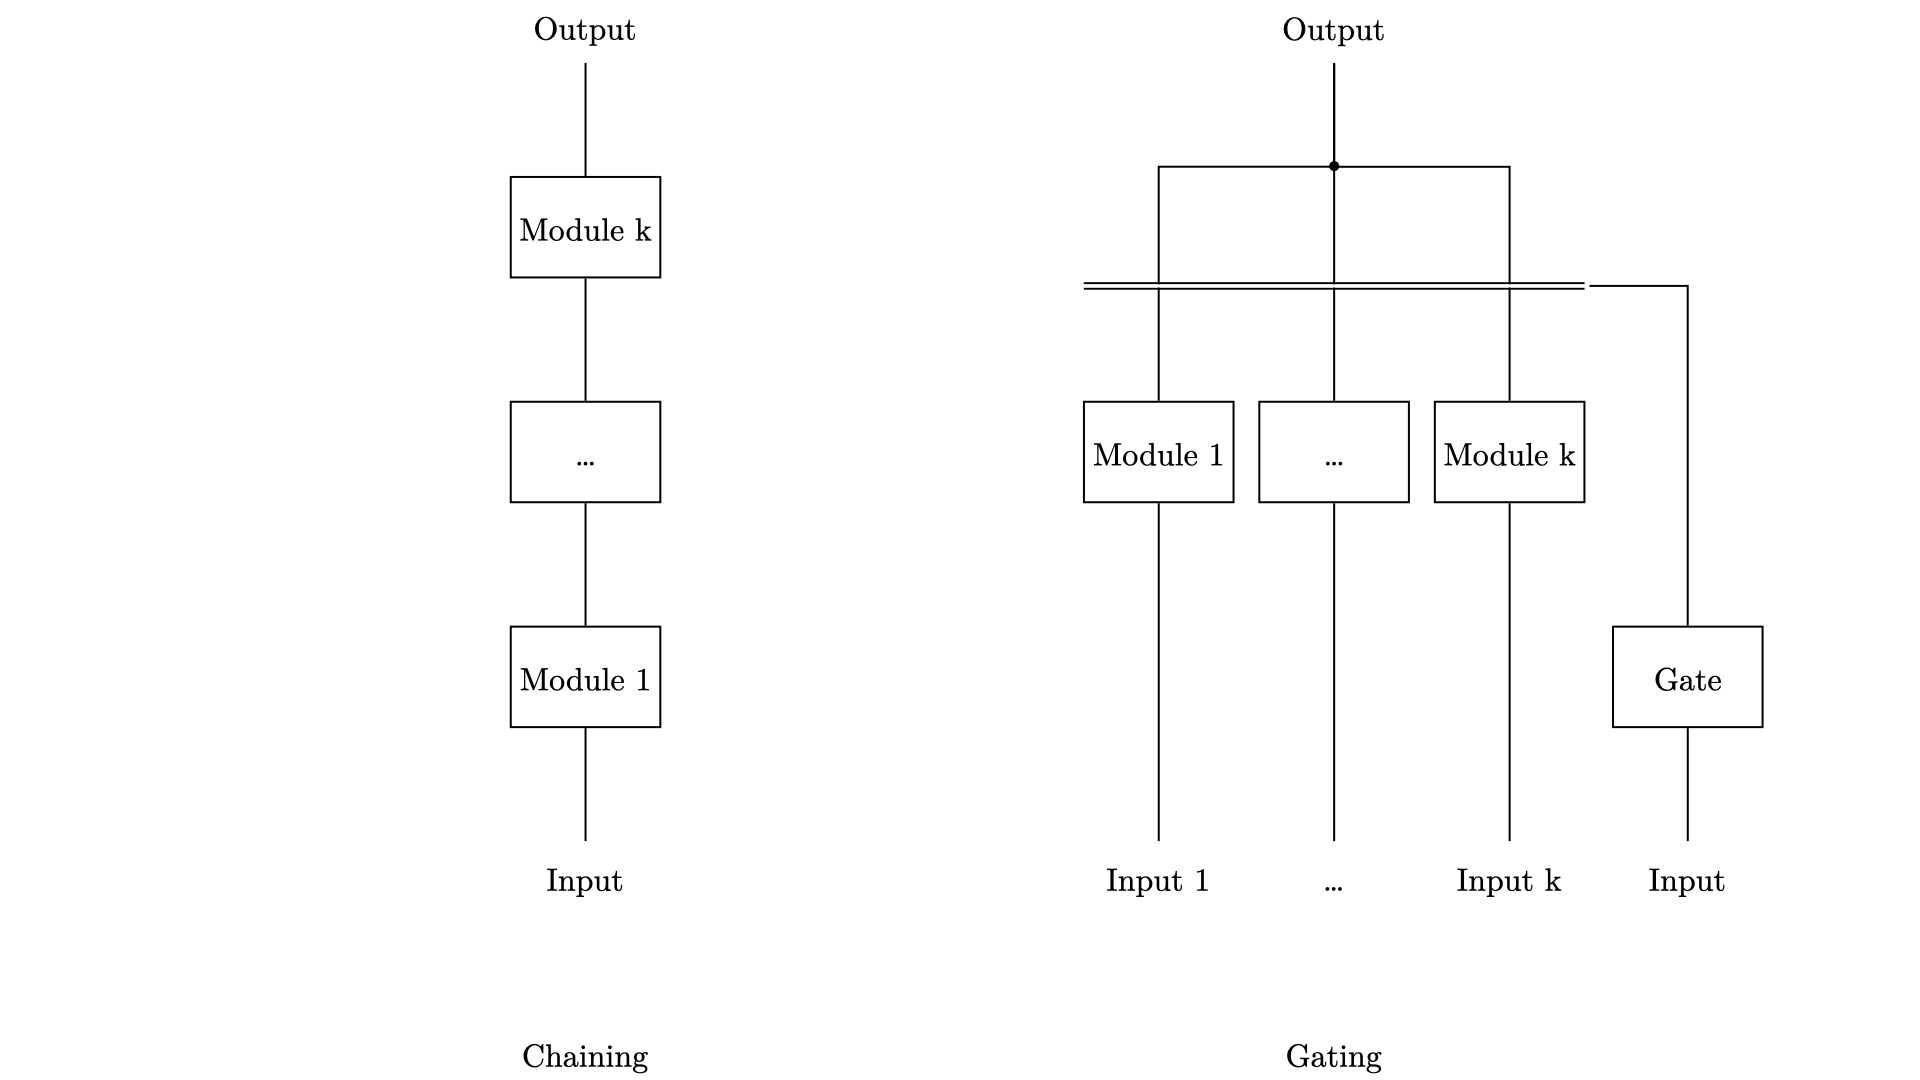
\includegraphics[width=\textwidth, trim=150 0 150 0, clip]{thesis/graphics/graphics/vertical_decomposition.jpeg}
    \caption{Common variants of vertical decomposition.}
    \label{fig:compnet_modularization_types_vertical_decomposition}
\end{figure}

\subsection{Modularization Error%
            \label{sec:compnet_error}}

A major challenge of modularization is finding a suitable decomposition that projects the prior knowledge concerning the structure of task or data base to the model without at the same time causing the loss of pivotal primary information e.\,g.\ due to oversimplification, etc. Noteworthily, the information is not really lost; the decomposition simply causes the network to lose the capability to model certain interrelations in this case due to the inferred constraints. Hence decomposition on the task and model layer can have adverse effects on the performance of the model if it decomposes the overall search space in a way that the theoretically optimal solution is located outside of the subspaces. We denote this as a suboptimal decomposition and the resulting deviation between theoretic optimum and closest reachable configuration within the composed search space as modularization error.

To further illustrate the basic problem, consider the following example. Imagine an auxiliary system for medical purposes that, based on the symptoms of a patient, tries to predict whether a person has a rheumatic fever. For this diagnosis, it is necessary that the patient was recently sick and either has a rash and arthralgia (joint pain) or a rash and a fever\footnote{Simplified for the sake of the example. In reality, there are several other possible symptoms.}. Consequently, the model is mapping from the symptom space $\{was\_sick,\ rash, arthralgia,\ fever\}$ to the diagnosis space $\{has\_rheumatic\_fever\}$. Now imagine a naive modularization that decomposes this system into four submodules that produce a partial prediction based on one of the symptoms each with the final diagnosis being formed by majority vote. Obviously, such a decomposition implicitly causes the system to lose the ability to model interrelations between the different symptoms and, as a result, combinations such as $was\_sick\ \wedge\ arthralgia\ \wedge\ fever\ \wedge\ \neg rash$ result in false positive predictions.

While the former example is of course highly simplified and it is easily visible that a better modularization would have been to decompose the system into two submodules $\{was\_sick,\ rash,\ arthralgia\}\rightarrow\{has\_rheumatic\_fever\}$ and $\{was\_sick,\ rash,$ $fever\}\rightarrow\{has\_rheumatic\_fever\}$ and combining the respective predictions with a deterministic \lstinline{or} block, this is only so because we have complete prior knowledge of the transformation. In reality, however, the latter is seldom or only partly known in advance, making it difficult to find a suitable modularization. In some cases, it may not even be possible to decompose the model without any simplifications and hence loss of information at all.

Furthermore, even if an optimal decomposition can be found, modularization may also affect the topology of the search space in a way that the inherent characteristics of optima finding algorithms -- most commonly SGD -- are affected negatively (e.\,g.\ by resulting in subspaces that are almost completely sparse). This may additionally impact efficiency and performance of the model.

Consequently, finding a suitable decomposition is a sensitive issue and should always be performed on a per-model basis for the performance loss due to modularization errors not to outweigh the practical advantages of a composed network.

\subsubsection{Propagation of Modularization Errors in different Types of Composition%
            \label{sec:compnet_error_propagation}}

As was argued in the previous section, it is rarely possible to decompose a model without inferring any error at all, i.\,e.\ without losing the capability to model certain interrelations in the data. If a model is now partitioned more than once, the errors of the individual decompositions compound. In this respect, we consider it to be of interest for practical applications to have an estimate of how the error develops with each further modularization, i.\,e.\ how much each additional decomposition deteriorates the overall model's performance.

In the following, we try to provide a qualitative analysis of error propagation in composed networks. We limit the scope of the analysis to the most common variants of horizontal and vertical modularization, in particular Additive Aggregation, Multiplicative Aggregation, Chaining and Gating. Furthermore, we do only consider such decompositions that result in DAGs.

It is generally assumed that the predictive distribution of a model $\hat{\textbf{p}}$ can be modeled as an additive superposition of the ground truth distribution $\textbf{p}$ and a diverging component $\boldsymbol{\epsilon}$ induced by the modularization. The resulting error is then proportional to the distance between $\hat{\textbf{p}}$ and $\textbf{p}$ and can e.\,g.\ be measured using KL (Kullback-Leibler) divergence as a metric.

To motivate the following analysis, once again consider a basic MLP. Given a set of data points $\textbf{X}$ with respective labels $\textbf{Y}$, our goal is to learn a transformation $f:\textbf{X}\rightarrow\textbf{Y}$. This is equivalent to fitting the predictive distribution $\textbf{p}(\textbf{y}|\textbf{X})$\footnote{We omit the dependency on the parameters of the model $\boldsymbol{\theta}$ for the sake of readability.}. The result is an approximation $\Tilde{\textbf{p}}(\textbf{y}|\textbf{X})$. For the sake of the argument, assume that the deviation between ground truth and predictive distribution be negligibly small, i.\,e.\ $
\Tilde{\textbf{p}}(\textbf{y}|\textbf{X})\approx\textbf{p}(\textbf{y}|\textbf{X})$.

If the MLP is horizontally cut in two at an arbitrary layer (resulting in a vertical modularization) after training we do still expect the composite model to output $\textbf{p}(\textbf{y}|\textbf{X})$ if we feed the input to the first network and then use its predictions as input to the second network. However, if the chosen decomposition is suboptimal in the sense of the preceding section, the predictive distribution of the overall model is likely to deviate from the ground truth distribution by an error $\boldsymbol{\epsilon}(\textbf{y}|\textbf{X})$ (formulated as a distribution as well) induced by the modularization.

\begin{figure}[tb]
    \centering
	    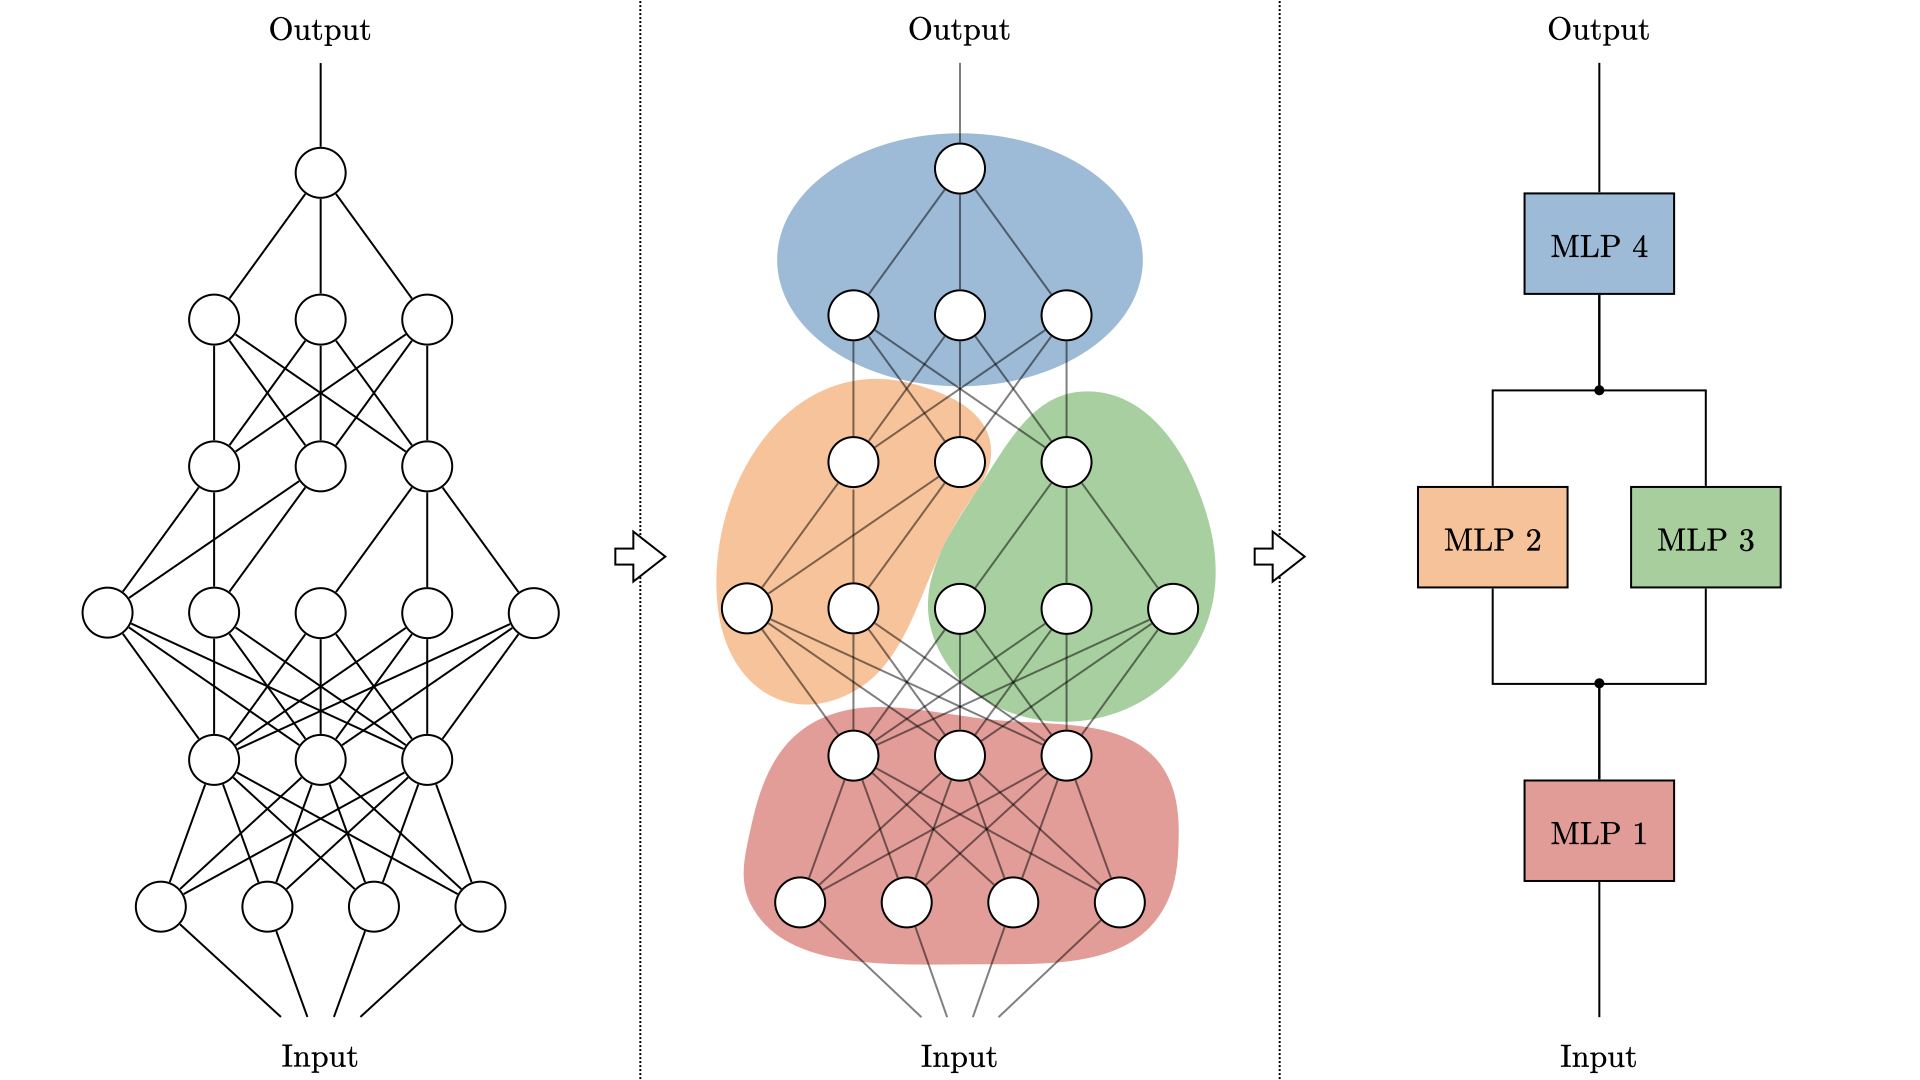
\includegraphics[width=\textwidth, trim=0 -25 0 -25, clip]{thesis/graphics/graphics/second_order_network.jpeg}
    \caption{Composite models can be interpreted as second-order networks with module-level nonlinearities similar to \cite{Lin2013-xh}. In the case that only MLPs are considered as activation functions, the overall model can be understood as a special form of pruning of a conventional network as depicted in the first two sections of the figure.}
    \label{fig:compnet_error_propagation_second_order_network}
\end{figure}

As depicted in figure \ref{fig:compnet_error_propagation_second_order_network}, the very same composed model can now also be interpreted as a second order neural network with the individual submodules as activation functions of the different neurons. From this analogy it can be concluded that

\begin{itemize}
    \item the total modularization error can be attributed proportionately to the individual submodules.
    \item the share of a submodule in the total error can be determined by iteratively tracing the error flow from the corresponding module to the final output analogous to backpropagation.
\end{itemize}

However, backpropagation, which traces the error flow backwards from the output to the module, requires knowledge about the derivation of the activation function of each neuron in the path which is not given in the case of module-level nonlinearities without having to make further assumptions about permissible submodule types. To obtain at least a qualitative understanding of how each decomposition affects the modularization error of the overall model we do therefore employ forward analysis in the following.

\pagebreak

\subsubsection{Modularization Error in Horizontal Decomposition}

\textbf{Additive Aggregation:} Consider $k$ parallel modules that all predict the same $\textbf{y}$. Let $\textbf{p}_{i}(\textbf{y}|\textbf{X}_i)$ denote the predictive distribution of the $i$-th submodule. Assuming additive aggregation, the overall predictive distribution can then be expressed as

\begin{equation}
\label{eq:compnet_error_propagation_add_dist}
    \textbf{p}(\textbf{y}|\textbf{X})\ =\ \sum_{i=1}^k\textbf{p}_i(\textbf{y}|\textbf{X}_i)
\end{equation}

Considering the additional modularization error $\boldsymbol{\epsilon}$ attributable to each horizontal decomposition, this becomes

\begin{equation}
\label{eq:compnet_error_propagation_add_dist_err}
    \textbf{p}(\textbf{y}|\textbf{X})+\boldsymbol{\epsilon}(\textbf{y}|\textbf{X})\ =\ \sum_{i=1}^k\textbf{p}_i(\textbf{y}|\textbf{X}_i)+\boldsymbol{\epsilon}_i(\textbf{y}|\textbf{X}_i)
\end{equation}

Consequently, it can be seen that each additional submodule adds the additional modularization error term $\boldsymbol{\epsilon}_i$.

\textbf{Multiplicative Aggregation:} Similar to before, consider $k$ parallel modules that all predict the same $\textbf{y}$ and let $\textbf{p}_{i}(\textbf{y}|\textbf{X}_i)$ denote the predictive distribution of the $i$-th submodule. Then, assuming multiplicative aggregation, the overall predictive distribution is

\begin{equation}
\label{eq:compnet_error_propagation_mult_dist}
    \textbf{p}(\textbf{y}|\textbf{X})\ =\ \prod_{i=1}^k\textbf{p}_i(\textbf{y}|\textbf{X}_i)
\end{equation}

Taking into account the error $\boldsymbol{\epsilon}$ induced by each individual module, this becomes

\begin{equation}
\label{eq:compnet_error_propagation_mult_dist_err}
    \textbf{p}(\textbf{y}|\textbf{X})+\boldsymbol{\epsilon}(\textbf{y}|\textbf{X})\ =\ \prod_{i=1}^k\textbf{p}_i(\textbf{y}|\textbf{X}_i)+\boldsymbol{\epsilon}_i(\textbf{y}|\textbf{X}_i)
\end{equation}

Adding a $k+1$-th submodule consequently impacts the overall predictive distribution as

\begin{equation}
\label{eq:compnet_error_propagation_mult_dist_err_additional_module}
\begin{split}
    [\textbf{p}_{1..k}(\textbf{y}|\textbf{X}_{1..k})+\boldsymbol{\epsilon}_{1..k}(\textbf{y}|\textbf{X}_{1..k})]\cdot[&\textbf{p}_{k+1}(\textbf{y}|\textbf{X}_{k+1})+\boldsymbol{\epsilon}_{k+1}(\textbf{y}|\textbf{X}_{k+1})]\ =\\
    & \textbf{p}_{1..k}(\textbf{y}|\textbf{X}_{1..k})\cdot\textbf{p}_{k+1}(\textbf{y}|\textbf{X}_{k+1})+\\
    & \textbf{p}_{1..k}(\textbf{y}|\textbf{X}_{1..k})\cdot\boldsymbol{\epsilon}_{k+1}(\textbf{y}|\textbf{X}_{k+1})+\\
    & \boldsymbol{\epsilon}_{1..k}(\textbf{y}|\textbf{X}_{1..k})\cdot\textbf{p}_{k+1}(\textbf{y}|\textbf{X}_{k+1})+\\
    & \boldsymbol{\epsilon}_{1..k}(\textbf{y}|\textbf{X}_{1..k})\cdot\boldsymbol{\epsilon}_{k+1}(\textbf{y}|\textbf{X}_{k+1})
\end{split}
\end{equation}

Comparing this expression to equation \ref{eq:compnet_error_propagation_mult_dist}, it can be seen that each further horizontal decomposition extends the overall modularization error by $\textbf{p}_{1..k}\cdot\boldsymbol{\epsilon}_{k+1}+\boldsymbol{\epsilon}_{1..k}\cdot\textbf{p}_{k+1}+\boldsymbol{\epsilon}_{1..k}\cdot\boldsymbol{\epsilon}_{k+1}$.

\subsubsection{Modularization Error in Vertical Decomposition}

\textbf{Chaining:} Let $\textbf{p}_{1}(\textbf{y}_1|\textbf{X})$ denote the predictive distribution of the first layer and $\textbf{p}_{i}(\textbf{y}_i|\textbf{y}_{i-1})$ the distribution of subsequent layers. Then the overall predictive distribution of $k$ consecutively chained layers can be expressed as

\begin{equation}
\label{eq:compnet_error_propagation_chaining_dist}
    \textbf{p}_k(\textbf{y}_k|\textbf{X})\ =\ \textbf{p}_k(\textbf{y}_k|\textbf{p}_{k-1}(\textbf{y}_{k-1}|..\textbf{p}_1(\textbf{y}_1|\textbf{X})))
\end{equation}

Under consideration of the modularization error $\boldsymbol{\epsilon}$ attributable to each vertical decomposition, this becomes

\begin{equation}
\label{eq:compnet_error_propagation_chaining_dist_err}
\begin{split}
    \textbf{p}_k(\textbf{y}_k|\textbf{X})+\boldsymbol{\epsilon}_k(\textbf{y}_k|\textbf{X})\ =\ &
    \textbf{p}_k(\textbf{y}_k|(\textbf{p}_{k-1}(\textbf{y}_{k-1}|..(\textbf{p}_1(\textbf{y}_1|\textbf{X})+\boldsymbol{\epsilon}_1(\textbf{y}_{1}|\textbf{X})))+\\
    &\ \ \ \ \ \ \ \ \ \ \boldsymbol{\epsilon}_{k-1}(\textbf{y}_{k-1}|..(\textbf{p}_1(\textbf{y}_1|\textbf{X})+\boldsymbol{\epsilon}_1(\textbf{y}_{1}|\textbf{X})))))+\\
    &\boldsymbol{\epsilon}_k(\textbf{y}_k|(\textbf{p}_{k-1}(\textbf{y}_{k-1}|..(\textbf{p}_1(\textbf{y}_1|\textbf{X})+\boldsymbol{\epsilon}_1(\textbf{y}_{1}|\textbf{X})))+\\
    &\ \ \ \ \ \ \ \ \ \ \boldsymbol{\epsilon}_{k-1}(\textbf{y}_{k-1}|..(\textbf{p}_1(\textbf{y}_1|\textbf{X})+\boldsymbol{\epsilon}_1(\textbf{y}_{1}|\textbf{X})))))
\end{split}
\end{equation}

Now, if an additional chained layer is added, using equation \ref{eq:compnet_error_propagation_chaining_dist_err} the subsequent predictive distribution can be expressed as

\begin{equation}
\label{eq:compnet_error_propagation_chaining_dist_additional_layer}
\begin{split}
    \textbf{p}_{k+1}(\textbf{y}_{k+1}|\textbf{X})+\boldsymbol{\epsilon}_{k+1}(\textbf{y}_{k+1}|\textbf{X})\ =\ &
    \textbf{p}_{k+1}(\textbf{y}_{k+1}|(\textbf{p}_k(\textbf{y}_k|\textbf{X})+\boldsymbol{\epsilon}_k(\textbf{y}_k|\textbf{X})))+\\
    & \boldsymbol{\epsilon}_{k+1}(\textbf{y}_{k+1}|(\textbf{p}_k(\textbf{y}_k|\textbf{X})+\boldsymbol{\epsilon}_k(\textbf{y}_k|\textbf{X})))
\end{split}
\end{equation}

Assuming a sensible decomposition resulting in a comparably small error and using first-order Taylor approximation, this can also be written as

\begin{equation}
\label{eq:compnet_error_propagation_chaining_dist_additional_layer_taylor}
\begin{split}
    \textbf{p}_{k+1}(\textbf{y}_{k+1}|\textbf{X})+\boldsymbol{\epsilon}_{k+1}(\textbf{y}_{k+1}|\textbf{X})\ =\ &
    \textbf{p}_{k+1}(\textbf{y}_{k+1}|(\textbf{p}_k(\textbf{y}_k|\textbf{X})))+\\
    & \textbf{p}_{k+1}(\textbf{y}_{k+1}|\boldsymbol{\epsilon}_k(\textbf{y}_k|\textbf{X})))+\\
    & \boldsymbol{\epsilon}_{k+1}(\textbf{y}_{k+1}|(\textbf{p}_k(\textbf{y}_k|\textbf{X})))+\\
    & \boldsymbol{\epsilon}_{k+1}(\textbf{y}_{k+1}|\boldsymbol{\epsilon}_k(\textbf{y}_k|\textbf{X})))
    \end{split}
\end{equation}

Comparing this with equation \ref{eq:compnet_error_propagation_chaining_dist} it can be concluded that each additional chained layer extends the overall modularization error by $\textbf{p}_{k+1}(\textbf{y}_{k+1}|\boldsymbol{\epsilon}_k)+  \boldsymbol{\epsilon}_{k+1}(\textbf{y}_{k+1}|\textbf{p}_k)+\boldsymbol{\epsilon}_{k+1}(\textbf{y}_{k+1}|\boldsymbol{\epsilon}_k)$, i.\,e.\ the impact of the error of all preceding layers on the ground truth distribution of the new layer, the error of the new layer on the ground truth distribution of the preceding layers and the error of the preceding layers on the error of the new layer.

\pagebreak

\textbf{Gating:} Let $\textbf{p}_{i,j}^m(\textbf{y}_i|\textbf{X}_{i,j})$ denote the predictive distribution of the $j$-th module of the $i$-th layer with $m$ categories (one for each module on the $i+1$-th layer resp.\ for each output category on the last layer). Let furthermore

\begin{equation}
\label{eq:compnet_error_propagation_gating_dist_layer_i}
    \textbf{P}_i^{m{\times}n}(\textbf{y}_i|\textbf{X}_i)\ =\ %
    \begin{bmatrix}
        \textbf{p}_{i,1}(\textbf{y}_i|\textbf{X}_{i,1}) & \textbf{p}_{i,2}(\textbf{y}_i|\textbf{X}_{i,2}) & .. & \textbf{p}_{i,n}(\textbf{y}_i|\textbf{X}_{i,3})
    \end{bmatrix}
\end{equation}

denote the matrix of the predictive distributions of all $n$ submodules on the $i$-th layer and define the permissible number of modules on the first layer to be one. The overall predictive distribution of $k$ consecutive Gating layers can then be computed as\footnote{We omit the dependency of ${p}_k$ on $\textbf{y}_{k-1}$, $\textbf{y}_{k-2}$, ..., $\textbf{y}_1$ in the notation for the sake of readability.}

\begin{equation}
\label{eq:compnet_error_propagation_gating_dist_complete}
    \bar{\textbf{p}}_k(\textbf{y}_k|\textbf{X}_k)\ =\ \textbf{P}_k(\textbf{y}_k|\textbf{X}_k)\times\bar{\textbf{p}}_{k-1}(\textbf{y}_{k-1}|\textbf{X}_{k-1})=\prod_{i=1}^{k}\textbf{P}_i(\textbf{y}_i|\textbf{X}_i)
\end{equation}

where each multiplication denotes a matrix-vector product (since $\textbf{P}_1$ is a $m{\times}1$ vector by above definition). Taking into account the modularization error $\boldsymbol{\epsilon}$ attributable to each submodule, equation \ref{eq:compnet_error_propagation_gating_dist_layer_i} becomes

\begin{equation}
\label{eq:compnet_error_propagation_gating_dist_err_layer_i}
    \begin{bmatrix}
        \textbf{p}_{i,1}(\textbf{y}_i|\textbf{X}_{i,1})\\
        \textbf{p}_{i,2}(\textbf{y}_i|\textbf{X}_{i,2})\\
        \threevdots\\
        \textbf{p}_{i,n}(\textbf{y}_i|\textbf{X}_{i,3})
    \end{bmatrix}^T+%
    \begin{bmatrix}
        \boldsymbol{\epsilon}_{i,1}(\textbf{y}_i|\textbf{X}_{i,1})\\
        \boldsymbol{\epsilon}_{i,2}(\textbf{y}_i|\textbf{X}_{i,2})\\
        \threevdots\\
        \boldsymbol{\epsilon}_{i,n}(\textbf{y}_i|\textbf{X}_{i,3})
    \end{bmatrix}^T\ =\ %
    \textbf{P}_i^{m{\times}n}(\textbf{y}_i|\textbf{X}_i)+\textbf{E}_i^{m{\times}n}(\textbf{y}_i|\textbf{X}_i)
\end{equation}

and equation \ref{eq:compnet_error_propagation_gating_dist_complete} therefore becomes

\begin{equation}
\label{eq:compnet_error_propagation_gating_dist_err_complete}
    \bar{\textbf{p}}_k(\textbf{y}_k|\textbf{X}_k)+\bar{\boldsymbol{\epsilon}}_k(\textbf{y}_k|\textbf{X}_k)\ =\ \prod_{i=1}^{k}\textbf{P}_i(\textbf{y}_i|\textbf{X}_i)+\textbf{E}_i(\textbf{y}_i|\textbf{X}_i)
\end{equation}

Adding a subsequent $k+1$-th layer impacts the overall predictive distribution as

\begin{equation}
\label{eq:compnet_error_propagation_gating_dist_additional_layer}
\begin{split}
    \bar{\textbf{p}}_{k+1}(\textbf{y}_{k+1}|\textbf{X}_{k+1})+\bar{\boldsymbol{\epsilon}}_{k+1}(\textbf{y}_{k+1}|\textbf{X}_{k+1})\ =\  &
    [\textbf{P}_{k+1}(\textbf{y}_{k+1}|\textbf{X}_{k+1})+\textbf{E}_{k+1}(\textbf{y}_{k+1}|\textbf{X}_{k+1})]\times\\
    & [\bar{\textbf{p}}_k(\textbf{y}_k|\textbf{X}_k)+\bar{\boldsymbol{\epsilon}}_k(\textbf{y}_k|\textbf{X}_k)]
\end{split}
\end{equation}

From the comparison with equation \ref{eq:compnet_error_propagation_gating_dist_complete} it becomes obvious that each additional layer extends the modularization error by $\textbf{P}_{k+1}\times\bar{\boldsymbol{\epsilon}}_k+\textbf{E}_{k+1}\times\bar{\textbf{p}}_k+\textbf{E}_{k+1}\times\bar{\boldsymbol{\epsilon}}_k$. This is equivalent to the additional error term of chaining, only that the individual components are not chained but instead multiplied in this case. Adding a further submodule to a layer similarly increases the error by $\textbf{p}_{k+1,n+1}\times\bar{\boldsymbol{\epsilon}}_{k,m+1}+\boldsymbol{\epsilon}_{k+1,n+1}\times\bar{\textbf{p}}_{k,m+1}+\boldsymbol{\epsilon}_{k+1,n+1}\times\bar{\boldsymbol{\epsilon}}_{k,m+1}$.

\subsubsection{Modularization Error in Mixed Decomposition}

\begin{figure}[htb]
    \centering
	    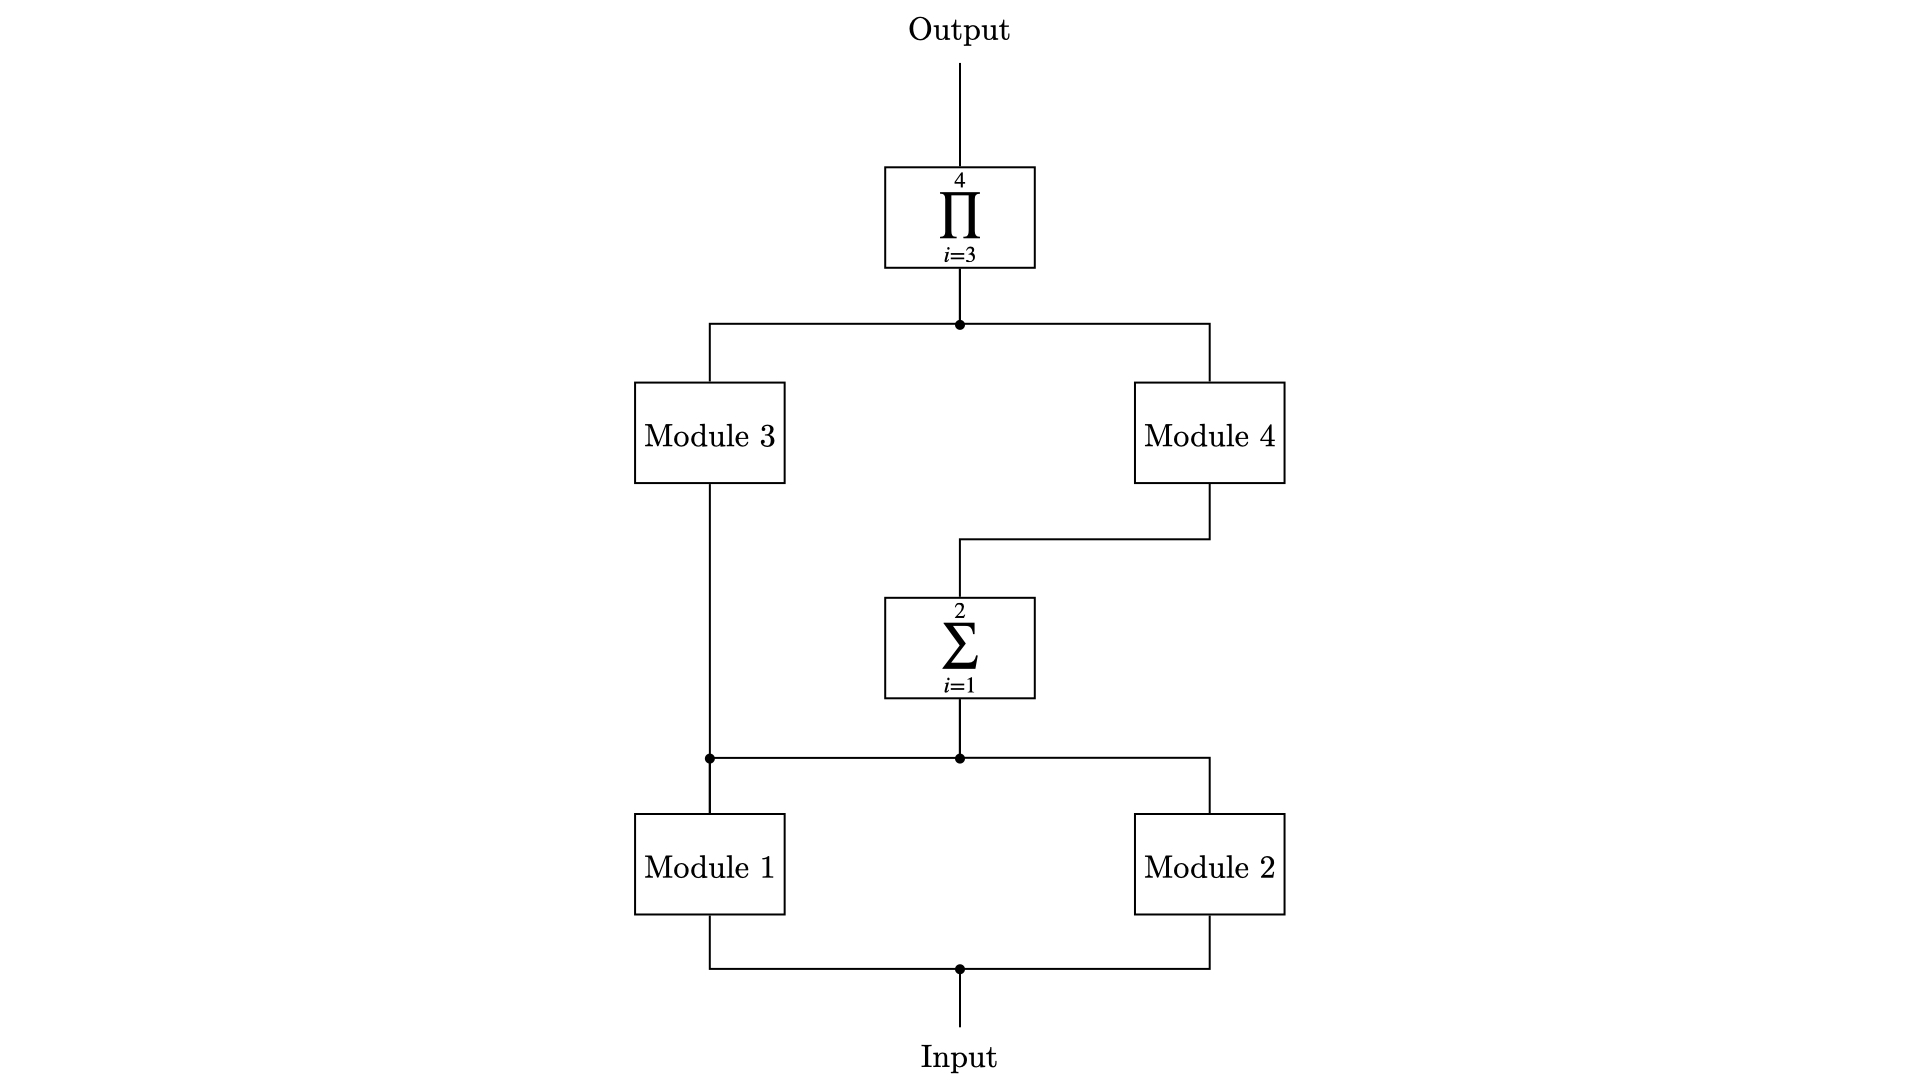
\includegraphics[width=\textwidth, trim=250 0 250 0, clip]{thesis/graphics/graphics/modularization_error_example.jpeg}
    \caption{Illustrative example of a composed network consisting solely of the above modularization types.}
    \label{fig:compnet_error_propagation_modularization_error_example}
\end{figure}

Now that the basic variants of decomposition have been studied, it is straightforward to transfer the findings to mixed modularizations. Following the above notion of a second-order network with module-level nonlinearities, the modularization error of a model arbitrarily partitioned in the above ways can be assessed on a qualitative basis by simply concatenating the error terms of the individual decompositions bottom-up in order of their occurrence.

Consider e.\,g.\ the meta-network depicted in figure \ref{fig:compnet_error_propagation_modularization_error_example}. Starting at the input layer, modules $M_1$ and $M_2$ induce the error $\boldsymbol{\epsilon}_1$ and $\boldsymbol{\epsilon}_2$ respectively. As $M_1$ is chained to $M_3$, the error is propagated as

\begin{equation*}
    \bar{\boldsymbol{\epsilon}}_3\ =\ %
    \textbf{p}_3(\textbf{y}_3|\boldsymbol{\epsilon}_1)+\boldsymbol{\epsilon}_3(\textbf{y}_1|\textbf{p}_1)+\boldsymbol{\epsilon}_1(\textbf{y}_3|\boldsymbol{\epsilon}_1)
\end{equation*}

on the left path. On the right path, the additive aggregation of $M_1$ and $M_2$ is input into $M_4$, translating to

\begin{equation*}
    \bar{\boldsymbol{\epsilon}}_4\ =\ %
    \textbf{p}_4(\textbf{y}_4|[\boldsymbol{\epsilon}_1+\boldsymbol{\epsilon}_2])+\boldsymbol{\epsilon}_4(\textbf{y}_4|[\textbf{p}_1+\textbf{p}_2])+\boldsymbol{\epsilon}_4(\textbf{y}_4|[\boldsymbol{\epsilon}_1+\boldsymbol{\epsilon}_2])
\end{equation*}

with regard to the modularization error. Finally, the outputs of $M_3$ and $M_4$ are multiplicatively aggregated to arrive at the final prediction, thus propagating the error of the preceding decompositions as

\begin{equation*}
    \boldsymbol{\epsilon}_5\ =\ %
    \textbf{p}_3\cdot\bar{\boldsymbol{\epsilon}}_4+\bar{\boldsymbol{\epsilon}}_3\cdot\textbf{p}_4+\bar{\boldsymbol{\epsilon}}_3\cdot\bar{\boldsymbol{\epsilon}}_4
\end{equation*}

Altogether, the overall error induced by the modularization can finally be expressed as

\begin{equation}
\label{eq:compnet_error_propagation_mixed_example}
\begin{split}
    \boldsymbol{\epsilon}_{total}\ =\  &
    \textbf{p}_3\cdot[\textbf{p}_4(\textbf{y}_4|[\boldsymbol{\epsilon}_1+\boldsymbol{\epsilon}_2])+\boldsymbol{\epsilon}_4(\textbf{y}_4|[\textbf{p}_1+\textbf{p}_2])+\boldsymbol{\epsilon}_4(\textbf{y}_4|[\boldsymbol{\epsilon}_1+\boldsymbol{\epsilon}_2])]+\\
    & [\textbf{p}_3(\textbf{y}_3|\boldsymbol{\epsilon}_1)+  \boldsymbol{\epsilon}_3(\textbf{y}_3|\textbf{p}_1)+\boldsymbol{\epsilon}_3(\textbf{y}_3|\boldsymbol{\epsilon}_1)]\cdot\textbf{p}_4+\\
    & [\textbf{p}_3(\textbf{y}_3|\boldsymbol{\epsilon}_1)+\boldsymbol{\epsilon}_3(\textbf{y}_3|\textbf{p}_1)+\boldsymbol{\epsilon}_3(\textbf{y}_3|\boldsymbol{\epsilon}_1)]\cdot\\
    & [\textbf{p}_4(\textbf{y}_4|[\boldsymbol{\epsilon}_1+\boldsymbol{\epsilon}_2])+\boldsymbol{\epsilon}_4(\textbf{y}_4|[\textbf{p}_1+\textbf{p}_2])+\boldsymbol{\epsilon}_4(\textbf{y}_4|[\boldsymbol{\epsilon}_1+\boldsymbol{\epsilon}_2])]
\end{split}
\end{equation}

In conclusion, we have shown that it is possible to isolate and to analytically express the errors induced by different kinds of decomposition. While this does still not allow for any statement regarding the concrete nature of the composed model's overall predictive distribution or its deviation from the ground truth, it provides a heuristic to assess the relative influence of each individual submodule on the performance of the meta-network on a more profound basis than pure counting of connections. Especially in situations with limited time or resources this can be useful to facilitate the decision where to focus first. E.\,g.\ from equation \ref{eq:compnet_error_propagation_mixed_example} in the above example it can be seen that $M_1$ impacts the model much more than the other submodules. In, for instance, a business scenario, it would hence be the natural decision to devote the available resources to the minimization of $\boldsymbol{\epsilon}_1$ before the others.

Although the derivation of the concrete error caused by a certain type of decomposition is beyond the scope of this work, we hope to have established a fundamental understanding of the qualitative influence of different forms of modularization on the performance of a composite model.

\cleardoublepage

\section{Experiments%
         \label{sec:experiments}}
         
\subsection{General Considerations%
            \label{sec:experiments_general}}

Now to examine the impact of modularization on learning behavior and detection rate of neural networks in practice, we performed a total of three experiments on four different datasets. All test cases involve image recognition using varying CNN architectures. Note that in doing so, we accept an inherent bias resulting from the similarity of the tasks which restricts the generalizability of our findings; nevertheless, the decision to still do so was due to the lack of usage-ready, empirically tested data in other areas that fit our requirements.

In particular, we evaluated the performance of each a model composed from several submodules and a comparable monolithic benchmark model on the CIFAR10 and CIFAR100 datasets \cite{Krizhevsky2009-wt}, the ImageNet animal subset \cite{Deng2009-iz}, as well as the CIFAR100-C corruption benchmark \cite{Hendrycks2019-gi} (described in more detail in the sections of the respective experiments), whereby "performance" is used as a collective term for various metrics describing the general learning behavior in this context in contrast to the conventional notion of predictive accuracy.

Since our utmost goal was the assessability of the proposed approach, we decided on several principles to maximize the comparability of our results that we took into consideration in the design of the different experiments. Most of them (should) hold true in almost any experiment in general; nevertheless, to enable the reader to better understand our decisions, we explicitly summarize them in the following:

\textbf{Scalability of the basic model architecture:} Since we employed the same basic architecture for the submodules of the composed network as well as for the respective benchmark model in each experiment for the sake of comparability, it was necessary that the architecture could be (down)scaled with a certain granularity.

\textbf{Simplicity / leanness of the basic model architecture:} Simplicity / leanness refers to the degree of prior knowledge inferred into the basic architecture. As we believe our approach to be orthogonal to approaches that infer knowledge through modifications of the atomic units composing the overall architecture (cf.\ e.\,g.\ residual units proposed in \cite{He2015-cq} that introduce additional shortcut connections to infer knowledge about the inherently sparse nature of image feature detectors), we deliberately avoided incorporating such elements into our work. This serves to keep the results as clean as possible with regard to clear attributability of observed effects and to reduce potential error vectors.

\textbf{Usage of established methodology:} Established methodology can be understood both in terms of the model as well as the training / testing procedure. Concerning the former, it is desirable to choose an architecture that has already successfully been tested on the respective datasets and for which reference values can be found in literature. Not only does this provide a means of cross-validation of one's own results; it also facilitates second degree comparability beyond the experiments described in the following sections. The same holds true for the training / testing procedure.

\textbf{Contemporary task complexity levels:} While the first three principles are important for the comparability of the results, the last aspect relates to the complexity of the problem space on the basis of which the experiments are carried out. Many techniques perform quite adequately on fairly trivial problems such as MNIST but do not generalize well to contemporary task complexity levels as introduced by datasets such as e.\,g.\ ImageNet because of scalability issues, etc. Thus, even though we do assume that the same qualitative results would have been observable on an easier task as well, models and datasets were chosen to reasonably reflect contemporary complexity to take this aspect into account.

We are aware that the aforementioned principles are at least partly in contravention with each other (e.\,g.\ most contemporary image recognition models incorporate a certain degree of prior knowledge about the problem statement in some way or other which is contradictory to the previous notion of simplicity). Nevertheless, we tried to achieve an acceptable compromise in this field of tension to the best of our abilities during the design of the different experiments.

Finally, it should be noted at this point, that, even though there are several promising approaches to be found in literature regarding possible improvements of the resilience of hierarchically composed models (cf.\ e.\,g.\ \cite{Fergus2010-or}, \cite{Deng2014-so} or \cite{Roy2020-rv}), we avoided incorporating these ideas into our experiments as the goal of this work is to examine whether modularization of networks in general is a feasible approach and we wanted to keep our results as unbiased as possible in this regard (i.\,e.\ not "unfairly" improving one approach in comparison to the other). Nevertheless, it should also be noted that in doing so, we leave lots of room for improvement.

In the following, we will now describe the different experiments in detail. Each section is structured in the same way and begins with a description of the content of the respective experiment as well as the metrics evaluated. Subsequently, a concise summary of each the dataset and the models is given, followed by a description of the training and testing procedure employed. The sections are concluded by a presentation of the results and a short discussion of the limitations of each experiment.

\subsection{CIFAR100%
            \label{sec:experiments_cifar100}}

\subsubsection{Overview%
               \label{sec:experiments_cifar100_overview}}
               
In the first experiment, the performance of a hierarchically composed network on the CIFAR100 dataset was evaluated and compared to a monolithic reference model.

In particular, the progress of the conventional performance metrics in the form of categorical accuracy, categorical crossentropy and AUC (Area Under the ROC (Receiver Operating Characteristics) Curve) were observed during the training procedure to gain insight into the learning process. The learned distributions and the transformations between the layers were examined in addition to the aforementioned metrics on the testing dataset to obtain a qualitative understanding of the effects of the modularization on the predictive behavior of the network. Furthermore, the semantic distance in accordance to \cite{Fergus2010-or} was measured as a heuristic for the average separability of meta-concepts (i\,e.\ the average hierarchy level on which errors do occur; higher values indicate closer relation to the ground truth). The latter is especially of interest as in many applications a prediction close to the ground truth (e.\,g.\ "calf" instead of "cattle") is preferable over one that is categorically very different (e.\,g.\ "gorilla"), i.\,e.\ the loss function is inherently soft.
               
\subsubsection{Dataset%
               \label{sec:experiments_cifar100_dataset}}

\begin{figure}[htb]
    \centering
	    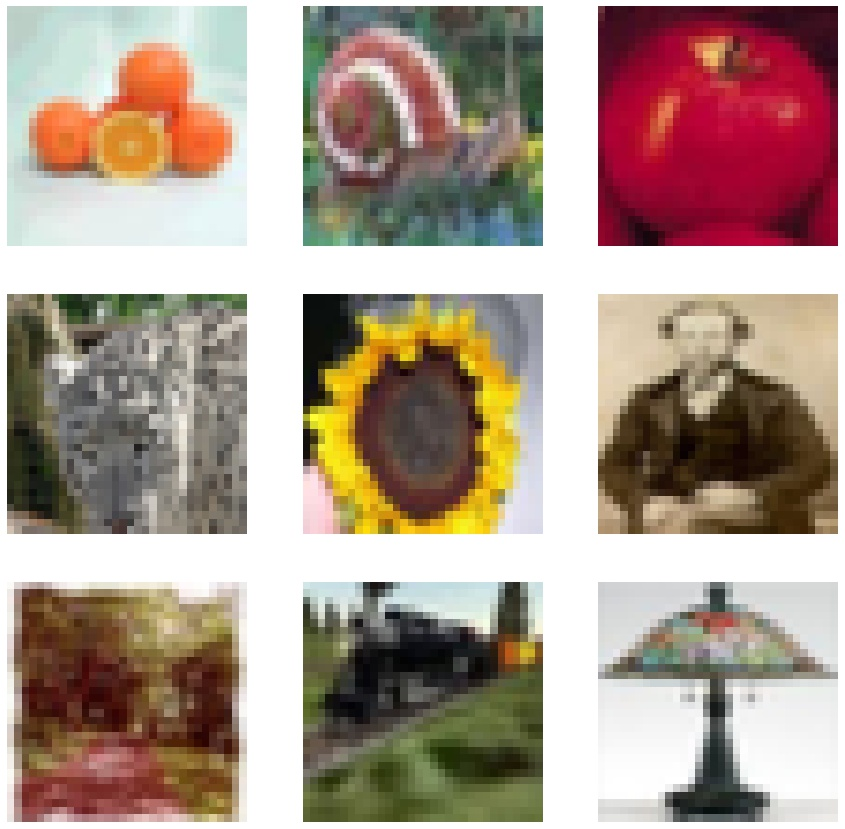
\includegraphics[width=\textwidth]{thesis/graphics/images/cifar100_sample_images.jpg}
    \caption{Randomly drawn (raw) sample images from the CIFAR100 dataset.}
    \label{fig:experiments_cifar100_sample_images}
\end{figure}
     
The CIFAR100 dataset is a subset of the tiny image dataset (\cite{Torralba2008-ah}) and was established by \cite{Krizhevsky2009-wt}. It consists of 60,000 32x32 pixel color (RGB) images in total (50,000 in the training and 10,000 in the testing subset) that have been manually labeled. A distinguishing property of this dataset is that it provides two different labels for each entry, denoted as "fine" and "coarse" labels. These categories are hierarchically connected, i.\,e.\ the coarse label specifies the meta-concept while the fine label represents the respective subcategory. There are 20 coarse concepts with each five unique fine categories, making for a total of 100 classes on the fine layer (cf.\ figure \ref{fig:experiments_cifar100_label_structure}). There is only one object in each sample. All records have been centered around the respective object which takes the main part of the image. Since its establishment, CIFAR100 has been widely used in research as a benchmark for image recognition models.

\subsubsection{Models%
               \label{sec:experiments_cifar100_models}}

\begin{table}
    \centering
    \begin{tabular}{|c|c|c|}
        \hline
        \textbf{Layer} & \textbf{Composed Network} & \textbf{Benchmark} \\
        \hline
        \multicolumn{3}{c}{} \\[-2ex]
        \hline
        1 & MaxOut (conv.) - 32 & MaxOut (conv.) - 128 \\
        \hline
        2 & MaxPool & MaxPool \\
        \hline
        3 & Dropout & Dropout \\
        \hline
        4 & MaxOut (conv.) - 64 & MaxOut (conv.) - 256 \\
        \hline
        5 & MaxPool & MaxPool \\
        \hline
        6 & Dropout & Dropout \\
        \hline
        7 & MaxOut (conv.) - 128 & MaxOut (conv.) - 512 \\
        \hline
        8 & Flatten & Flatten \\
        \hline
        9 & Dropout & Dropout \\
        \hline
        10 & MaxOut (FC) - 64 & MaxOut (FC) - 256 \\
        \hline
        11 & Dropout & Dropout \\
        \hline
        12 & Softmax & Softmax \\
        \hline
        \multicolumn{3}{c}{} \\[-2ex]
        \hline
        \textbf{Parameters} & 2,353,172 & 37,538,912 \\
        \hline
    \end{tabular}
    \caption{Architectures of the submodules of the composed network and the reference model (FC = Fully Connected).}
    \label{tab:experiments_cifar100_models_structure}
\end{table}

Under consideration of the aforementioned principles (cf.\ section \ref{sec:experiments_general}), it was decided to use the MaxOut architecture as described by \cite{Goodfellow2013-za} as the reference architecture for both the composed and the benchmark model in this experiment. While not state of the art from today's perspective, it can still be said to achieve contemporary performance levels on various established image recognition benchmarks. The authors explicitly report their own results for the MNIST, CIFAR10, CIFAR100 and SVHN datasets where they all achieved SOTA (State Of The Art) at the time of the initial publication. The results have since then been reproduced by various independent sources (mostly as a comparative benchmark for novel approaches) such as \cite{Lin2013-xh}. Furthermore, with regard to the aforementioned principle of simplicity / leanness, the architecture meets the requirements as the main novelty of the approach is of purely mathematical nature and does not induce any prior knowledge of the problem task itself\footnote{Aside from the general implication that the decision boundaries between classes are of complex nature.}.

Additionally, the distinctive documentation of the MaxOut network in the original publication (i.\,e.\ the concrete model employed to arrive at the results described by \cite{Goodfellow2013-za}; not to be confused with the general concept of MaxOut units) facilitated the re-implementation for both the submodules of the composite network and the benchmark model (cf.\ below).

The meta-structure of the composed network adhered to that of the dataset as shown in figure \ref{fig:experiments_cifar100_label_structure}. We trained a total of 21 modules, one module for the coarse layer and for each subcategory. Except for the number of outputs that differed based on the layer, all submodules were kept identical. As depicted in table \ref{tab:experiments_cifar100_models_structure}, each model consisted of a total of three convolutional MaxOut layers with 32, 64 and 128 units each, kernel size 3x3, stride 1x1 and MaxOut resolution 8 (i.\,e.\ one MaxOut unit interpolates the superposition of eight linear functions). Each convolutional layer was connected to a MaxPool layer with pooling size and stride 2x2 and dimension preserving padding.

\pagebreak

\begin{figure}[htb]
    \centering
	    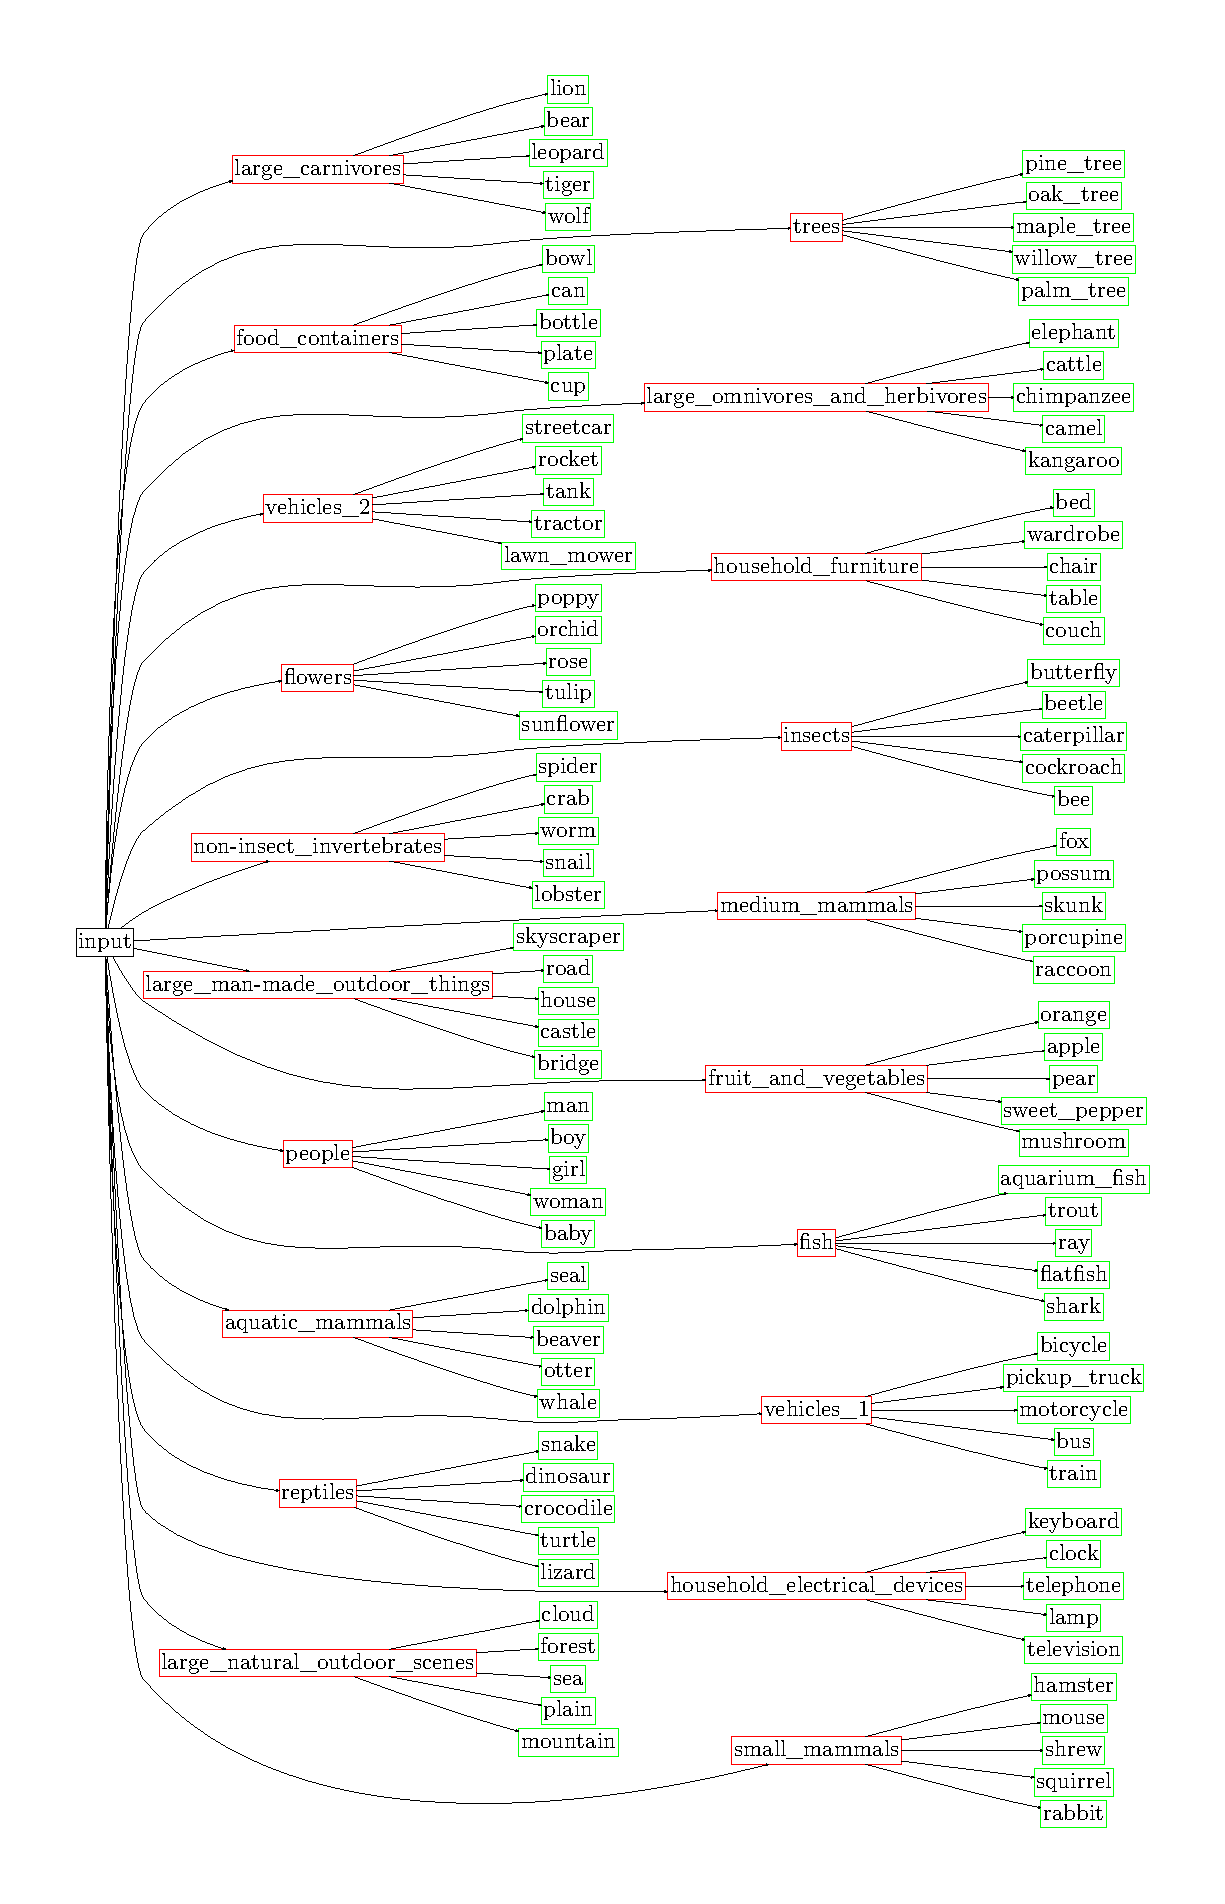
\includegraphics[width=\textwidth]{thesis/graphics/diagrams/cifar100_label_structure.pdf}
    \caption{Label structure of the CIFAR100 dataset. Colors indicate hierarchy levels.}
    \label{fig:experiments_cifar100_label_structure}
\end{figure}

\clearpage

After flattening the output of the last convolutional layer it was forwarded to a fully connected MaxOut layer with 64 units and MaxOut resolution 4, followed by the softmax output layer with the number of units equal to the number of classes on the respective hierarchy level (i.\,e.\ 20 on the coarse and 100 on the fine layer). For weight regularization, a combination of Dropout preceding and subsequent to the fully connected layer with activation rate $0.5$ and MaxNorm as \cite{Srivastava2014-pi} report to be most effective was employed. Furthermore, Dropout was also applied to the convolutional layers with an activation rate of $0.1$ to facilitate the discovery of informative features as described in \cite{Park2017-og}. All modules combined, the composed model possessed a total of 49,525,812 trainable weights.

The structure of the benchmark model followed the same basic architecture with the difference that the convolutional layers consisted of 128, 256 and 512 and the fully connected layer of 256 units respectively, making for a total of 37,538,912 trainable parameters.

The number of trainable weights was used as a factor for the comparability of the models here as we do assume that if two networks have roughly the same amount of DOFs -- in this case factor \char`\~1.3 in favor of the composed network -- they do possess a roughly equivalent modelling capability; thus the approach with the better results is the one that makes better / more efficient use of the given resources. Even though there are some adverse effects such as e.\,g.\ described in the first section of \cite{He2015-cq}, we do still deem it sufficient as a heuristic for comparability.

The reported hyperparameters in both cases were reached by starting off from sensible initial values and continuously improving them through empirical testing over several test runs until the results were in roughly the same order of magnitude as those reported by \cite{Goodfellow2013-za}. It should be noted though that no excessive optimization of the parameters was performed as our goal was not to try to compete for SOTA but rather to achieve a fair comparison between the composed and the benchmark model.
               
\subsubsection{Training%
               \label{sec:experiments_cifar100_training}}

For training, the original CIFAR100 training set was split up into a training and a validation set at a ratio of 4:1, i.\,e.\ 40,000 and 10,000 records respectively. Preprocessing and augmentation of both datasets was done in adherence to a slightly modified version of the standard 10-crop procedure as described by \cite{Krizhevsky2012-jr}.

Specifically, each image was one-hot encoded. Afterwards, global contrast correction and ZCA (Zero Component Analysis) whitening for decorrelation of pixel values (\cite{Krizhevsky2009-wt}, \cite{Goodfellow2013-za}) was applied to the one-hot encoded dataset as a whole. Each image was then repeated once and the duplicate was horizontally flipped. In combination with a subsequent extraction of five 28x28 pixel crops at random offsets per image this increased the size of the training set by a total factor of 10. This differs from the standard 10-crop procedure in which augmentation is instead achieved through random alterations of the intensities of the RGB channels of each image after flipping and random cropping (cf.\ section \ref{sec:experiments_imagenet_training} for a more detailed explanation). As the last step of preprocessing, the dataset was shuffled and batched with a batch size of 32 records per batch.

Training was done using categorical crossentropy as the loss function. Weight updates were performed using Adam (cf.\ \cite{Kingma2014-db}) with $\beta_1 = 0.9$, $\beta_2 = 0.999$ and $\epsilon = 1e-7$ as the optimizer. The learning rate was set dynamically depending on the training epoch, beginning with an initial rate of $1e-3$ which was lowered to $1e-4$ after the third and to $1e-5$ after the tenth epoch for the submodules of the composed network resp.~$1e-4$, $1e-5$ and $1e-6$ for the benchmark model. To avoid overfitting, early stopping with a minimum loss delta on the validation set of $1e-2$ and a patience of three epochs was employed during the whole training. Weight updates were performed until either convergence of the validation loss or 100 epochs; the latter was never reached though since the submodules of the composite as well as the benchmark network each converged after a maximum of 20 epochs.

As mentioned before, categorical accuracy, categorical crossentropy and AUC were recorded throughout the whole training procedure.

The values of the aforementioned hyperparameters were reached by several iterations of empirical testing and subsequent manual improvement; no excessive optimization was performed.

\subsubsection{Testing%
               \label{sec:experiments_cifar100_testing}}
               
The preprocessing of the testing dataset followed the same basic procedure as described for the training and validation set in the previous section for the most part. However, instead of performing random crops, the five crops were extracted at all four corners as well as the center for all images and no shuffling was performed. Also, the batch size was set to a fixed 10 records per batch so that each batch contained all augmentations of exactly one source image (five crops with horizontal reflections each). Predictions were then calculated by feeding all images of a batch to the model and subsequently averaging the individual scores.

In the case of the composed network, the batches were first evaluated on the coarse-layer model. Afterwards, they were fed to the fine-layer module with the maximum coarse-layer score, i.\,e.\ $max(\textbf{p}_{coarse})$, as a specific form of Gating (cf.\ section \ref{sec:compnet_modularization_types}). The prediction of the fine-layer module was then used as the final prediction of the network for evaluation.

During testing, the absolute distribution of predictions, the distribution of fine-level predictions per fine-level ground truths, the distribution of coarse-level predictions per coarse-level ground truths, as well as the distribution of fine-level predictions per coarse-level ground truths were measured in addition to semantic distance, categorical accuracy, categorical crossentropy and AUC\footnote{Similar to the other experiments, all results can be found in digital format on the attached CD (cf.\ appendix \ref{sec:appendix_digital}).}.
               
\subsubsection{Results \& Discussion%
               \label{sec:experiments_cifar100_results}}

\begin{table}
    \centering
    \begin{tabular}{|l|c|c|}
        \hline
        \textbf{Metric} & \textbf{Composed Network} & \textbf{Benchmark} \\
        \hline
        \multicolumn{3}{c}{} \\[-2ex]
        \hline
        Categorical Accuracy & 0.36 & 0.53 \\
        \hline
        Categorical Crossentropy & 6.51 & 1.78 \\
        \hline
        AUC & 0.79 & 0.96 \\
        \hline
        Semantic Distance (avg.) & 0.48 & 0.59 \\
        \hline
    \end{tabular}
    \caption{Results of the composed network and the benchmark model on the testing dataset.}
    \label{tab:experiments_cifar100_results_comparison}
\end{table}

The results of the evaluation of the composite network and the benchmark model on the testing dataset are shown in table \ref{tab:experiments_cifar100_results_comparison}.

We achieved a top-1 categorical accuracy of 35.69\% and 53.19\% with the composed resp.\ the benchmark model. As expected, the former performed worse than the monolithic network; nevertheless, it still comes comparably close, especially when considering that the individual submodules were all trained independently without subsequent finetuning of the meta-network. 

Similarly, the average semantic distance of the composed network is lower with 0.48 in comparison to 0.59 as well, however not by as much as the difference in performance would suggest (1.49x better performance in comparison to only 1.23x higher semantic distance). Hence, even though the benchmark model makes fewer errors, its wrong decisions are relatively further off than those of the composite network. In other words, by learning higher-level concepts, the predictions of the latter are on average contextually closer to the ground truth.

Nevertheless, the fact that the benchmark model comes so close relatively to the composite network and even outperforms it in absolute terms supports the thesis that, given enough time and resources, monolithic networks as universal approximators are able to learn categorical relationships equally well. I.\,e., while manual modularization reduces the amount of information a composite model has to learn by explicitly defining the inherent structure of the data base and hence provides an advantage in early stages of the training, this dissolves in a fully-converged comparison.

\begin{figure}[b!]
    \centering
	    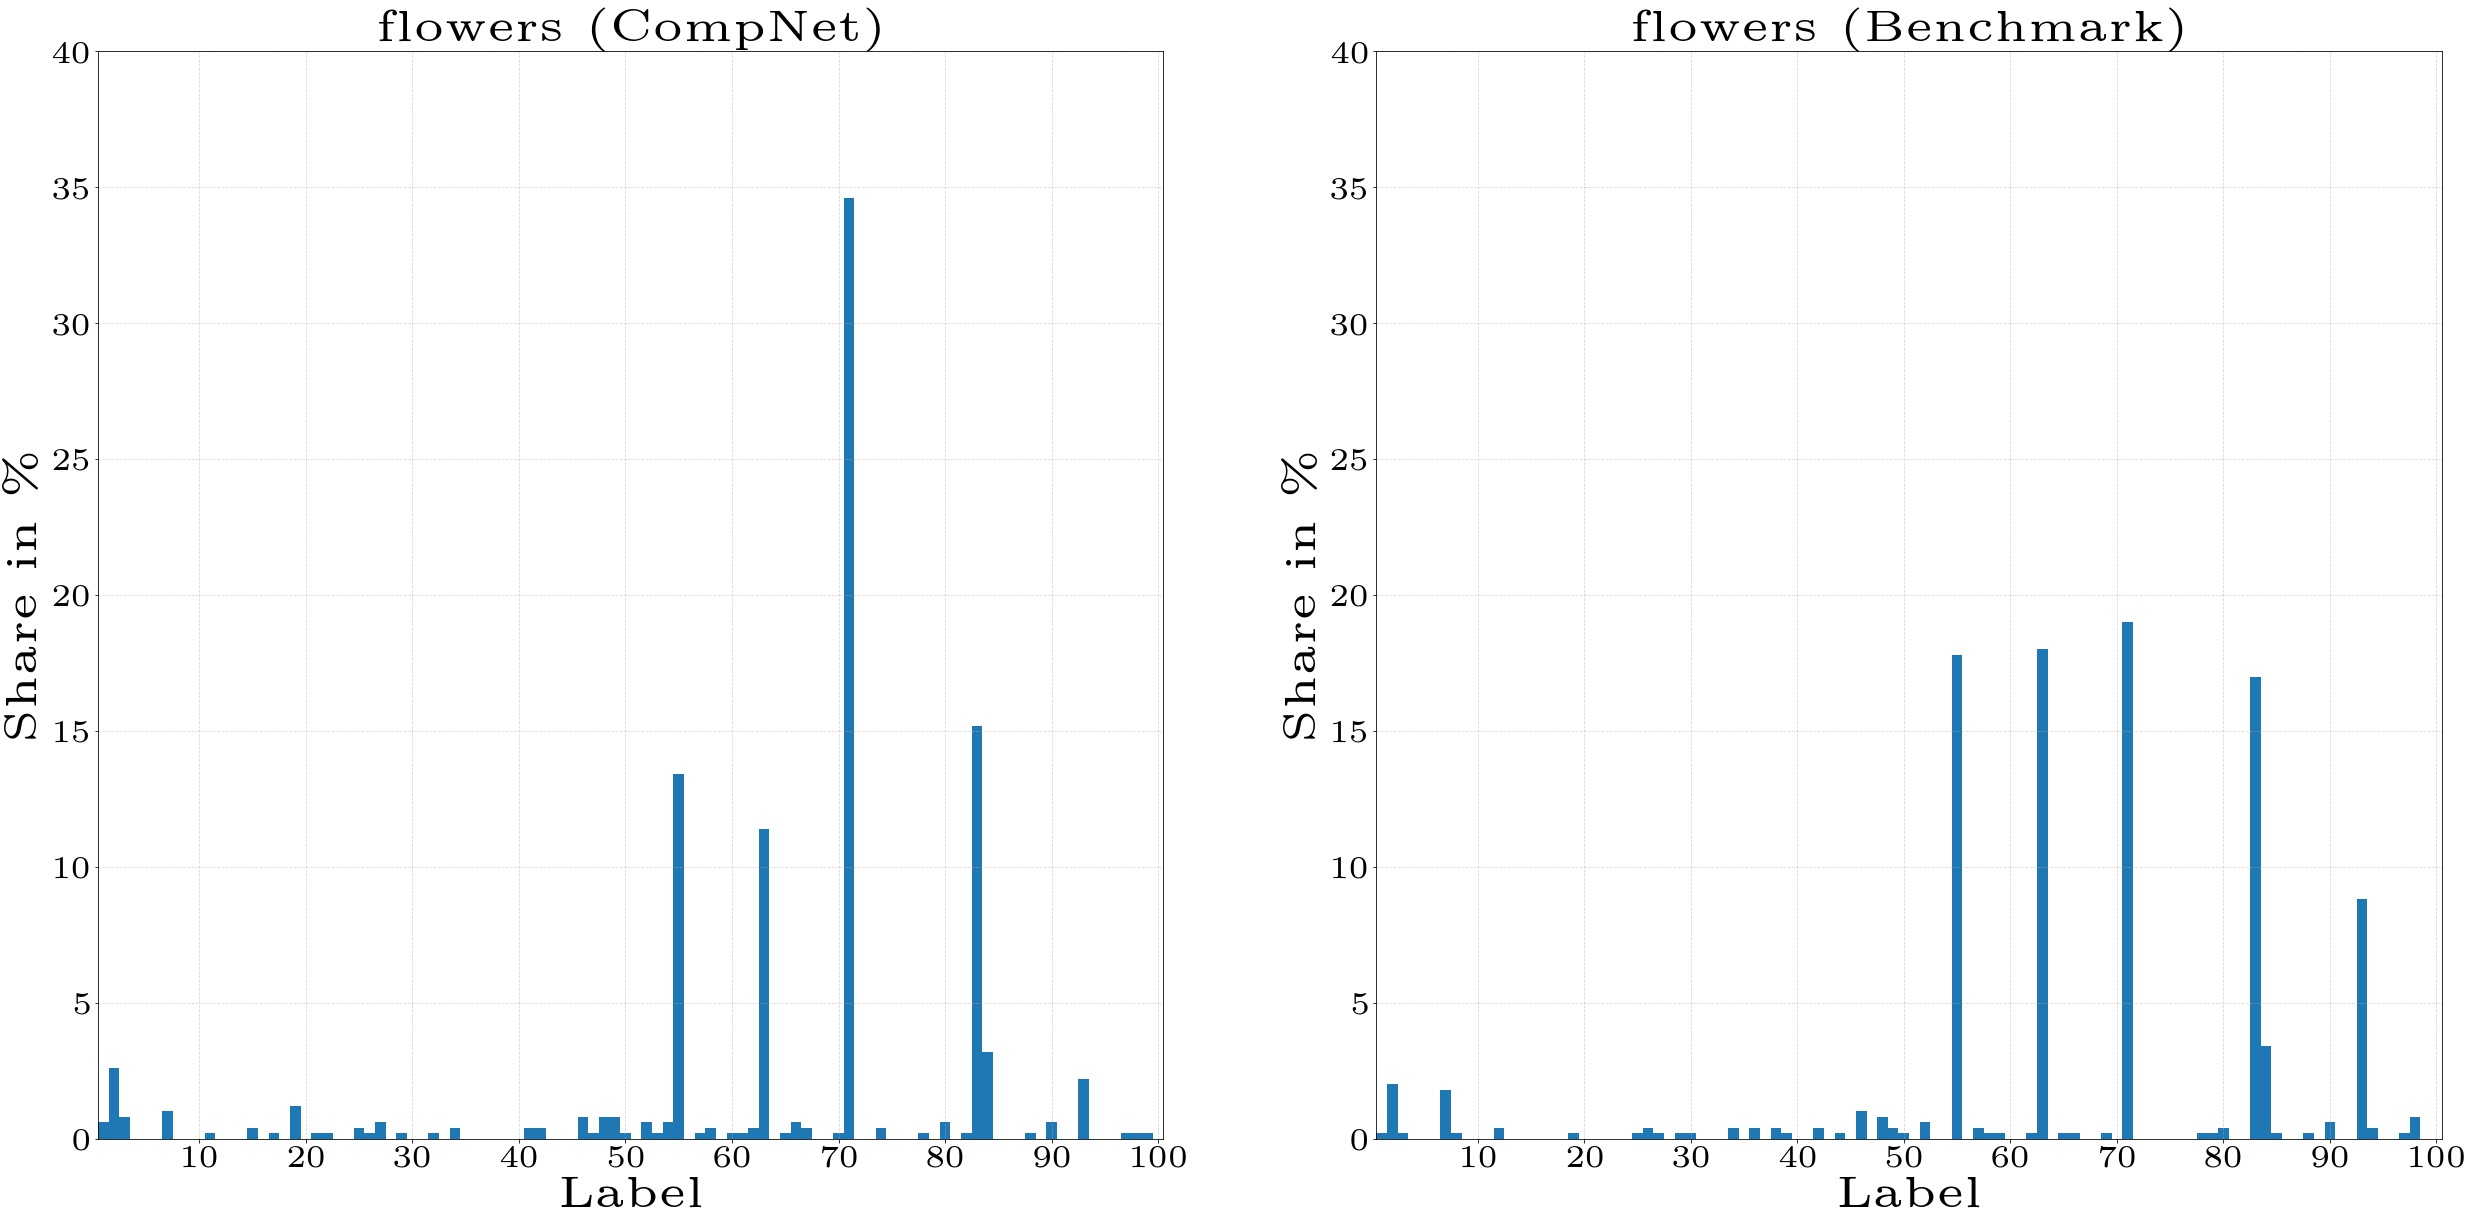
\includegraphics[width=\textwidth, trim=0 0 0 -50, clip]{thesis/graphics/diagrams/cifar100/cifar100_compnet_benchmark_dist_pred_fine_flower_print.jpg}
    \caption{Extract of the learned predictive fine-level distributions of composed and reference model for the same coarse category. Both learn widely similar distributions for the same meta-class.}
    \label{fig:experiments_cifar100_results_predictive_distribution_compnet_benchmark_fine_per_coarse_ground_truth}
\end{figure}

The categorical crossentropy and the AUC of the composed network also deviate significantly with regard to its monolithic counterpart with 6.51 and 0.79 in comparison to 1.78 and 0.96. We hypothesize this is due to the fact that only the fine-layer module that received the maximum score from the coarse-layer module is considered in the final prediction which results in the tails of the individual predictive distributions being "cut off".

To further examine this, we repeated the evaluation on the testing set for the composite model, this time constructing the fine-layer prediction from the scores of all submodules, each scaled by their respective coarse-layer score. In consequence, the crossentropy dropped to 2.49 while the AUC increased to 0.92, thus confirming our assumptions. However interestingly, the categorical accuracy and the semantic distance stayed almost constant with only minor improvements both. We presume this is due to softmax activation at the output layer of the coarse-level submodule which results in an over-emphasis of the prediction of the fine-level module that received the maximum score, thus making it hard for errors on the higher level to be compensated on the lower level.

Generally, the concatenation of (soft)max functions seems to result in amplification of imbalances within the predictive distributions of the individual submodules. Disparity on the coarse label level leads to certain modules on the fine label level being invoked disproportionately often, which in turn leads to their imbalance being reflected more strongly in the overall prediction distribution. This is catalyzed by the fact that the label spaces of the fine-layer submodules are mutually exclusive, leaving them with only the options to assign either the closest or the most prevalent category of their respective label space to images mistakenly shown to them due to misclassifications at the coarse-level module. E.\,g.\ one of ten examples for "man" is mistaken for "large omnivores and herbivores" instead of "people", resulting in the respective submodule commonly classifying these images as "chimpanzee". This is also reflected in figure \ref{fig:experiments_cifar100_results_predictive_distribution_compnet_benchmark}.

\begin{figure}[b!]
    \centering
	    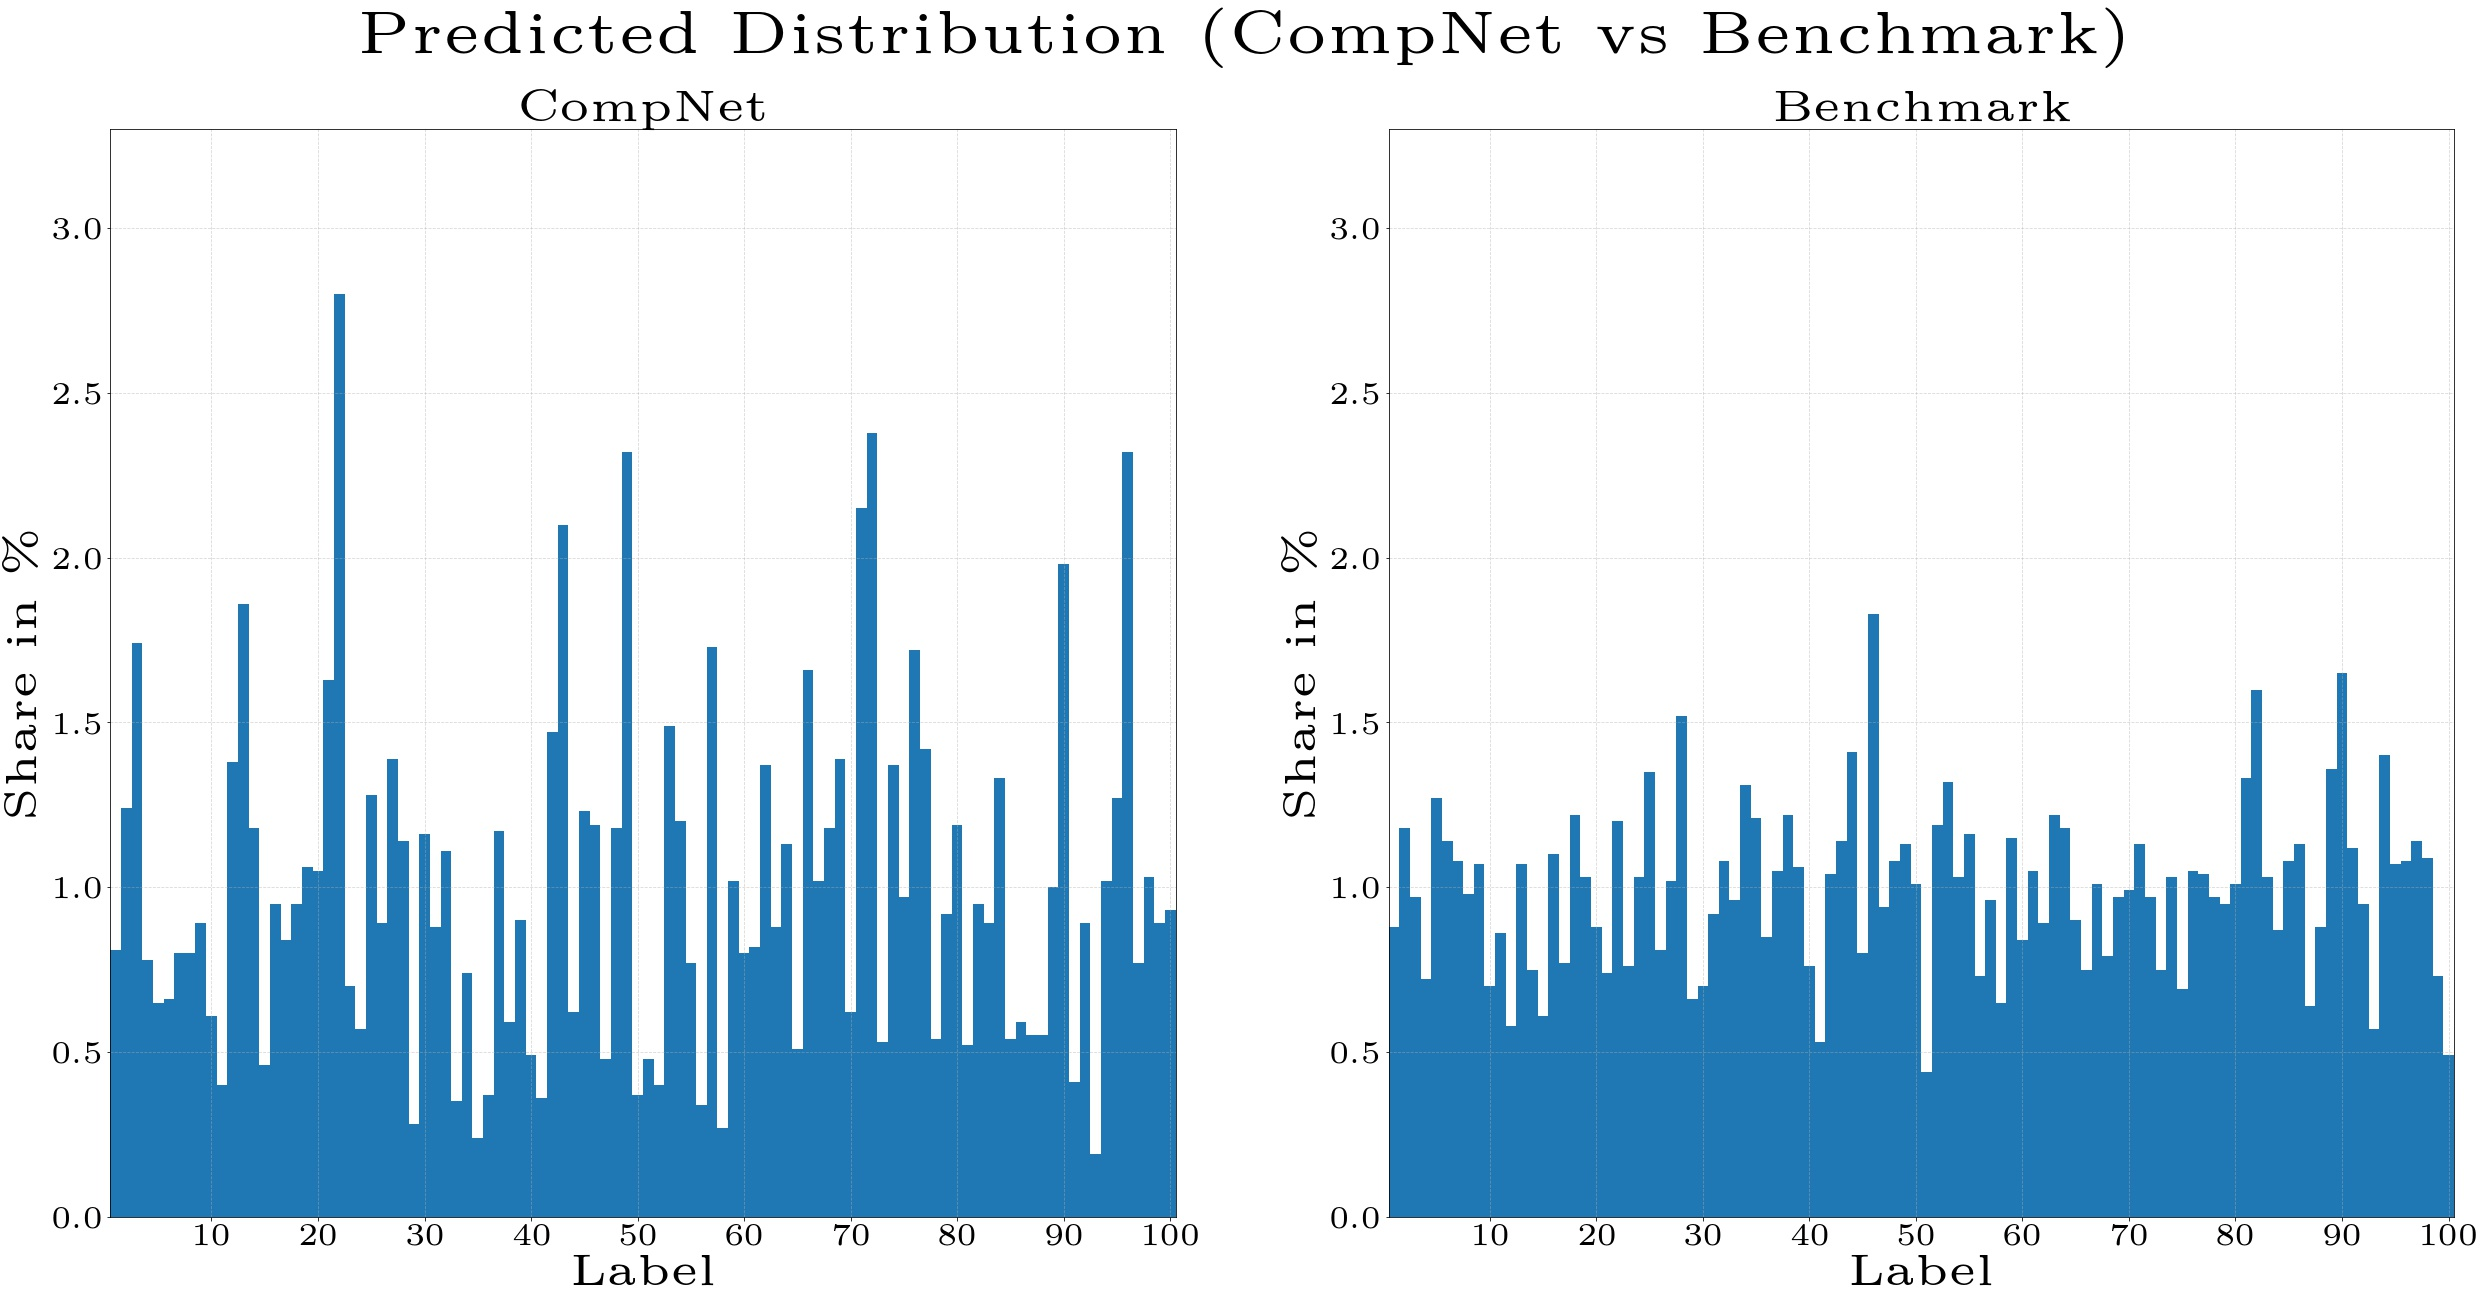
\includegraphics[width=\textwidth, trim=0 0 0 -50, clip]{thesis/graphics/diagrams/cifar100/cifar100_compnet_benchmark_dist_pred_print.jpg}
    \caption{Comparison between the learned predictive distributions of composed and benchmark model.}
    \label{fig:experiments_cifar100_results_predictive_distribution_compnet_benchmark}
\end{figure}

\subsubsection{Limitations%
               \label{sec:experiments_cifar100_limitations}}
               
As mentioned before, no excessive optimization of neither the composed nor the benchmark model was performed. Thus, even though this experiment serves as a foundation for a qualitative comparison between both approaches, no direct quantitative assessment can be made.

As a general limitation concerning the architecture of the composed network as was used in this experiment, with regard to all previously discussed forms of model combinations (cf.\ section \ref{sec:compnet_modularization_types}), Layering -- in particular Gating -- was the only form of decomposition employed. As a consequence, the above findings should be taken with a grain of salt when generalizing to modularization as a technique in general.
            
\subsection{ImageNet Animal Subset%
            \label{sec:experiments_imagenet}}
            
\subsubsection{Overview%
               \label{sec:experiments_imagenet_overview}}
               
In the second experiment, similar to the first, the performance of a hierarchically composed network was evaluated and compared to a monolithic benchmark model. However, instead of CIFAR100, the disproportionally more complex ILSVRC2012 animal subset was used as the reference dataset. The goal of this experiment was to assess the general applicability of the proposed approach, i.\,e.\ to evaluate whether the results from the first experiments can be qualitatively reproduced on a completely different dataset with a different reference network architecture. Furthermore, since the ImageNet animal subset infers a sufficient number of hierarchical layers, we examined the propagation of modularization errors in the composed network.

Again, we recorded categorical accuracy, categorical crossentropy and AUC, as well as the learned distributions and the transformations between the layers. Similar to the first experiment, semantic distance was measured as a heuristic of the hierarchical layer on which errors do happen on average in the composed network. The only new metric that was record is the top-5 accuracy which is commonly used to report a model's performance on more complex datasets like ImageNet.
               
\subsubsection{Dataset%
               \label{sec:experiments_imagenet_dataset}}

\begin{figure}[tb]
    \centering
	    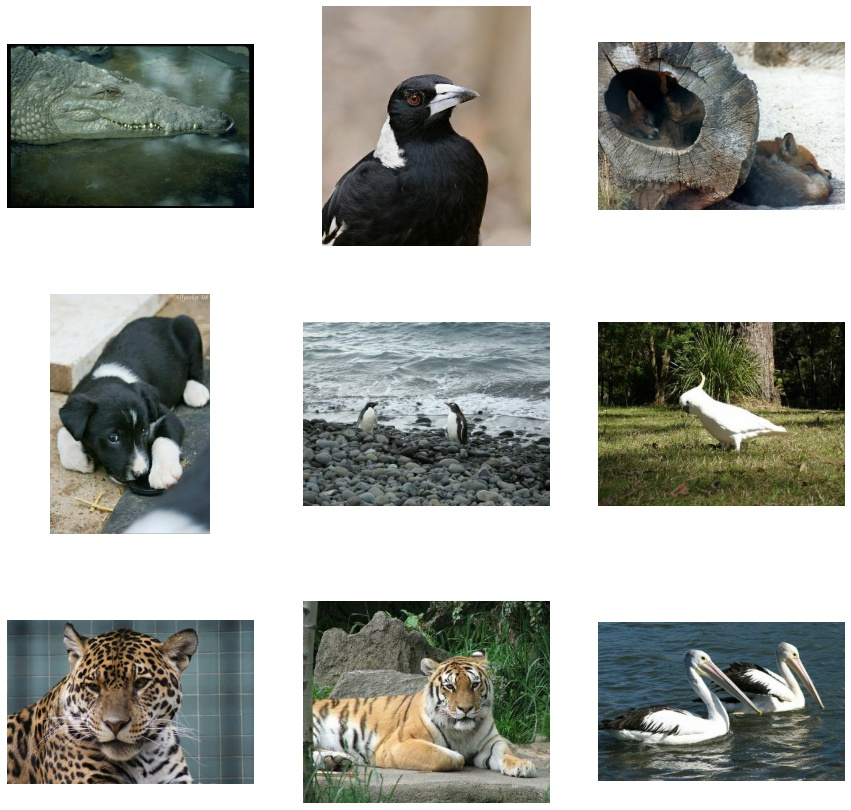
\includegraphics[width=\textwidth]{thesis/graphics/images/ilsvrc2012_as_sample_images.jpg}
    \caption{Randomly drawn (raw) sample images from the ILSVRC2012 animal subset.}
    \label{fig:experiments_imagenet_sample_images}
\end{figure}               

ImageNet is a large scale hierarchical image database and was established by \cite{Deng2009-iz}. It is built upon the structure of WordNet, a lexical database grouping cognitive synonyms of the English language into so called synsets and defining conceptual relations between them. ImageNet strives to provide an average of 1000 examples to each of the 80,000+ synsets and is continually advanced. Images are collected using various search engines on the internet and subsequently manually cleaned and labelled.

Since ImageNet itself is not well suited as a benchmark for image recognition models because of its inherently developing nature, a yearly competition called ILSVRC (ImageNet Large Scale Visual Recognition Challenge) has been held between 2010 and 2017 in which a fixed subset has been assembled by the organizers for researchers to compare their models' performance on. Of these, the ILSVRC2012 dataset is the most commonly used and has become a de facto standard for comparing progress in object detection and localization models in the last few years. It consists of a total of 1,331,167 color (RGB) images of varying resolution that are divided into 1000 different categories, each represented by a distinct WordNet synset and interrelated through their mutual conceptual parents (e.\,g.\ "terrier" and "hound" are related by their common hypernym (parental synset) "dog"). The records are not necessarily centered around the respective object of relevance and it is possible for the latter to be partly obscured.

To reduce the complexity of the task, primarily necessitated by limitations regarding the available computing power for training, we focused solely on the animal subset of the ILSVRC2012 dataset in this experiment (i.\,e.\ all categories with the common hypernym "animal"). The latter makes up about one third of the complete dataset.

We manually created a hierarchical label structure suited for the creation of a composed network from the underlying WordNet structure and cleaned the dataset in this regard. This mainly included removing ambiguous hypernym paths\footnote{A hypernym path is the list of all parental categories of a certain synset up to the topmost synset, in this case "animal". Since some labels such as "primate", which denotes not only a taxonomic category but also a religious title, have ambiguous meaning, it was necessary to remove unwanted synset paths.} and trimming all paths to have the same length (i.\,e.\ same number of parental categories) by identifying hypernyms commonly shared by as many synsets as possible and dropping scarcely populated ones. In doing so, we roughly followed the structure of the biological taxonomies.

Synsets with only one or less associated native labels from the original dataset were removed from the total set of hyponyms (filial synsets) of "animal". E.\,g.\ the hyponym "trilobite" of the synset "arthropod" has exactly one associated native label and would thus not permit any choice on the second hierarchy level in comparison to e.\,g.\ "arachnid" with nine labels and was dropped in consequence. This affected a total of 20 of 398 native labels (\char
`\~5\%).

Although it was tried to adhere to the underlying WordNet structure as far as possible in this process, some adjustments to the native hierarchy were necessary to balance out the distribution of the dataset to not unfairly put the composed approach at a disadvantage in comparison to the (monolithic) benchmark architecture:

\begin{itemize}
    \item Split up the native category "mammals" into smaller subcategories "dog", \\ "large\_omnivore\_herbivore", "ursine", "primatenic" and "other\_mammal"
    \item Aggregated native categories "coelenterate", "echinoderm", "mollusk" and "worm" into supercategory "molluscan"
    \item Aggregated native categories "amphibian" and "reptile" into supercategory "herpetologic"
\end{itemize}
 
These changes effect that each hypernym above the native labels possesses more than one direct filial category and does thus permit the training of a classification model. Moreover, they ensure that the maximum spread in the amount of data points per concept between the category with the most and the one with the least associated records on any hierarchy level is limited to a factor of < 15 (\char`\~5.5 on the root layer, \char`\~8.5 on the first layer and \char`\~15 on the second layer) to ensure that all submodules of the same level see a roughly similar number of records during training.

The resulting synset structure is depicted in figure \ref{fig:experiments_imagenet_label_structure}. The final dataset after applying the described changes to the original ILSVRC2012 animal subset consisted of 504,239 examples of 378 classes in total (388,200 training, 97,139 validation and 18,900 testing images) with roughly uniform distribution.
               
\subsubsection{Models%
               \label{sec:experiments_imagenet_models}}
               
With due regard to the same principles as before, it was decided to utilize the VGG architecture, initially established by \cite{Simonyan2014-bt}, for the construction of both the submodules of the composed as well as the benchmark network. This decision essentially follows the argumentation presented in section \ref{sec:experiments_cifar100_models} in relation to the decision to employ MaxOut in the first experiment. However, the VGG architecture is arguably better suited for more complex image recognition tasks such as ImageNet because of its higher modeling

\pagebreak

\begin{figure}[htb]
    \centering
	    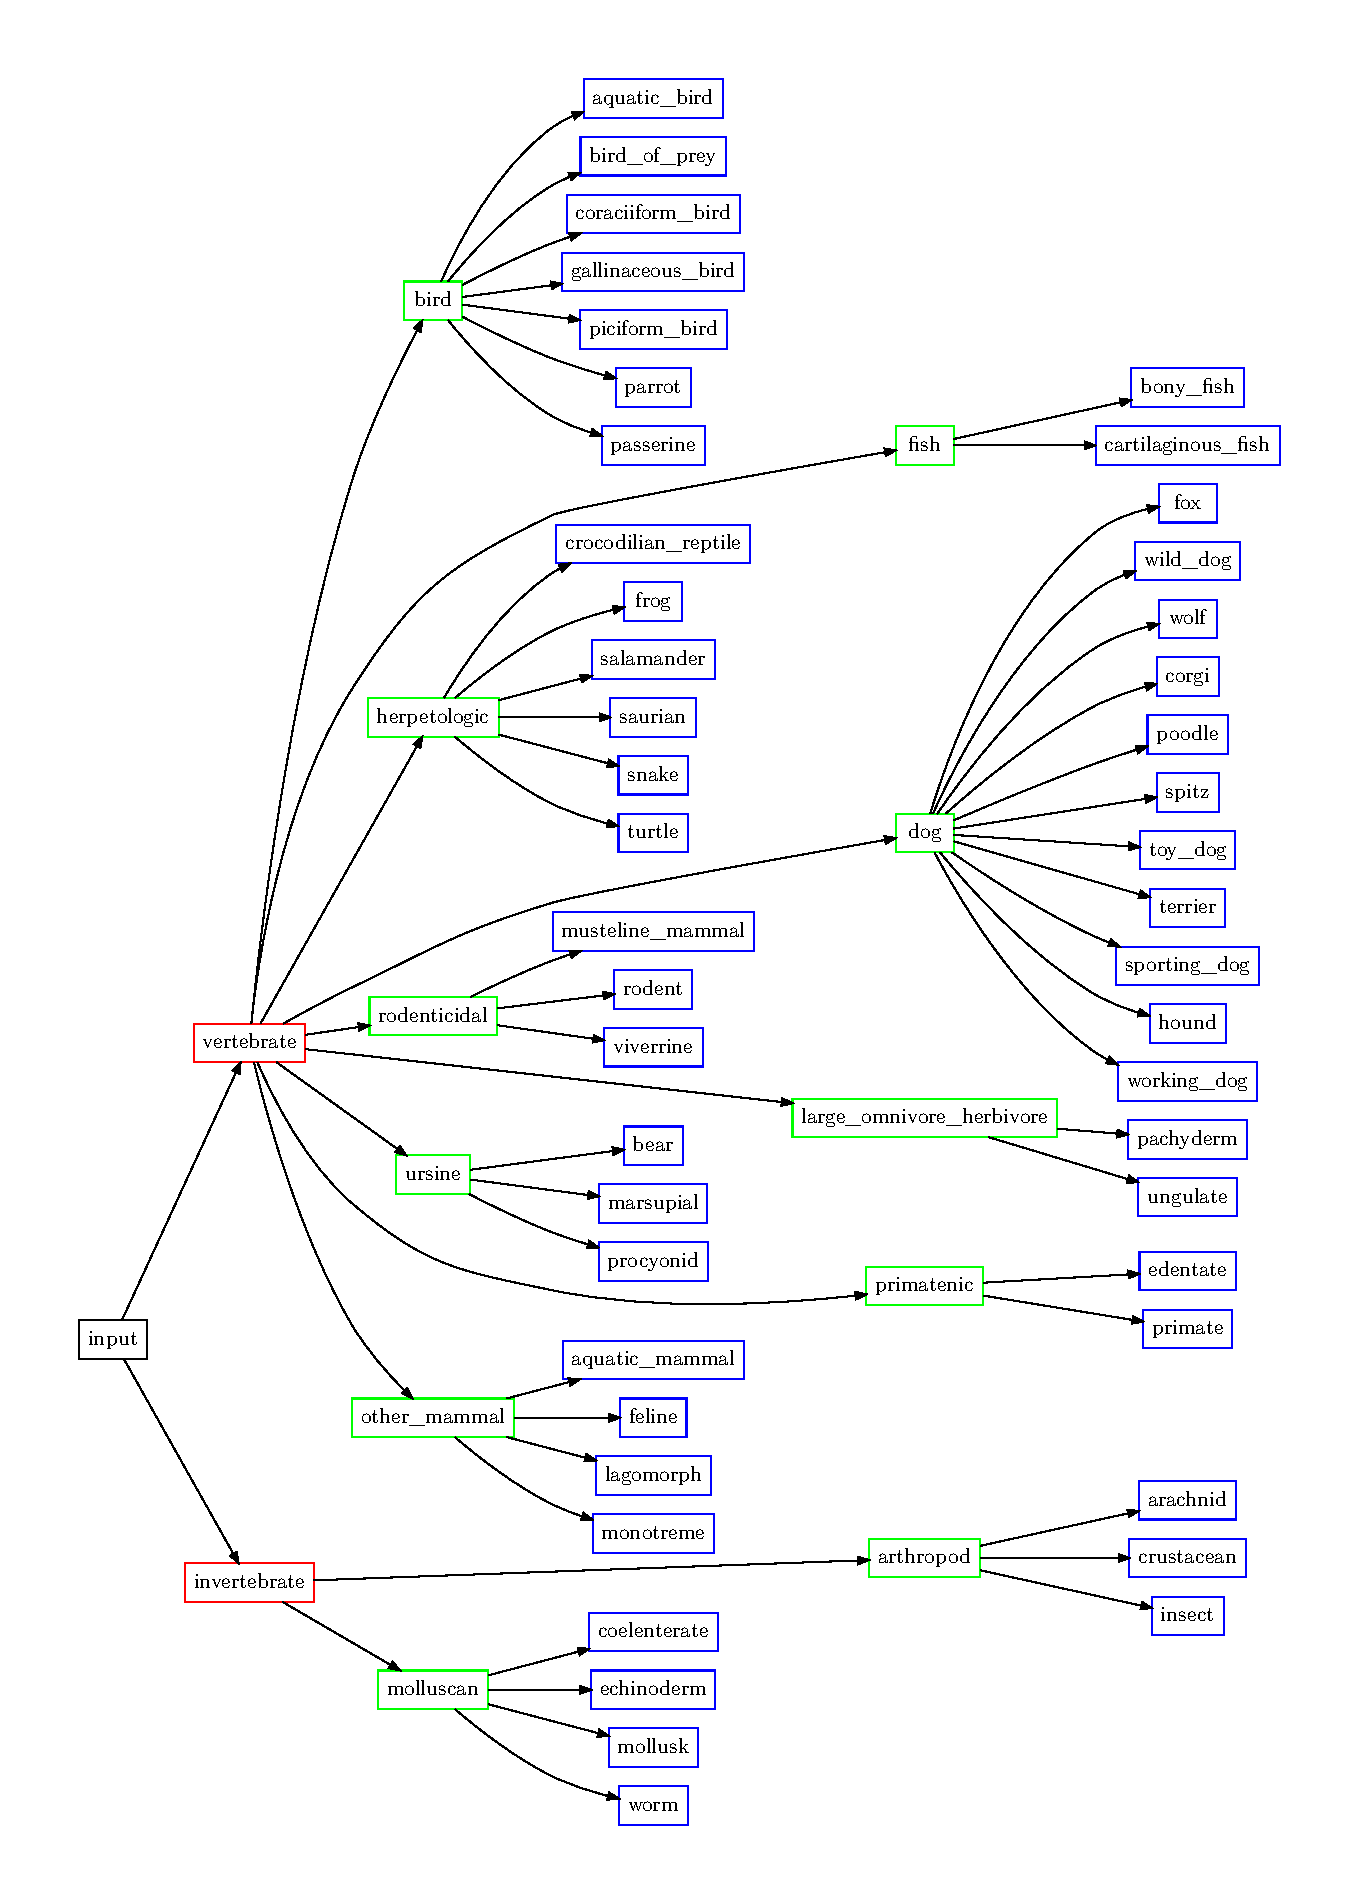
\includegraphics[width=\textwidth]{thesis/graphics/diagrams/ilsvrc2012_as_label_structure.pdf}
    \caption{Label structure of the ILSVRC2012 animal subset. The fourth layer containing the native dataset labels was excluded for the sake of readability. Colors indicate hierarchy levels.}
    \label{fig:experiments_imagenet_label_structure}
\end{figure}

\clearpage

capacity (again, under assumption of the latter's proportionality to the number of model parameters). Furthermore, since part of the goal of this experiment was to assess the model-independent applicability of our approach, it was decided to use a different reference architecture as before.

The meta-structure of the composed network adhered to the structure of the label space of the dataset. We trained one model for each non-leaf node in figure \ref{fig:experiments_cifar100_label_structure}, making for a total of 61 submodules on four hierarchical layers -- one on the topmost, two on the second, 11 on the third and 47 on the fourth layer. Except for the number of outputs that differed based on the number of direct hyponyms of the respective module, the structure of all submodules was kept identical and adhered to a downscaled version of the VGG11 architecture as depicted in table \ref{tab:experiments_imagenet_models_structure}.

Specifically, each module consisted of eight convolutional and two fully connected layers with a subsequent softmax output layer. The convolutional layers had 32, 64, 128, 128, 256, 256, 256 and 256 channels each with a pooling size of 3x3, stride 1x1 and dimension preserving padding. The first, second, fourth and sixth layer were furthermore connected to a MaxPool layer with pooling size 2x2 and stride 2x2. The fully connected layers consisted of 128 units each. ReLu was used as the activation function at all layers. This differs slightly from the original VGG11 architecture described by \cite{Simonyan2014-bt} and was done in order to keep the total number of trainable parameters of the composed network comparable to the benchmark model (cf.\ below). This reduction of parameters was mainly possible because each of the submodules only had to differentiate between up to 30 different classes in contrast to the 1000 categories the original reference model was dimensioned for, thus drastically reducing the complexity of each module's search space.

For weight regularization, a combination of Dropout preceding and subsequent to the fully connected layers with activation rate $0.5$ as well as L2 penalty at all layers with the regularization factor set to $5e-4$ was utilized. Additionally, Dropout was also applied to the convolutional layers with an activation rate of $0.1$ subsequent to the MaxPool layers. All modules combined, the composed model possessed a total of 239,654,970 trainable parameters.

The structure of the benchmark network strictly followed the VGG19 architecture with 16 convolutional layers with 64, 64, 128, 128, 256, 256, 256, 256, 512, 512, 512, 512, 512, 512, 512 and 512 channels respectively and two fully connected layers with 4096 units each. MaxPooling and Dropout were applied after the second, forth, eighth and twelfth convolutional layer. Aside from that, the remaining configuration was kept identical to the composed network. All in all, the benchmark model had a total of 141,118,906 trainable weights.

Again, we used the number of trainable weights as a heuristic for the comparability of the models following the reasoning presented in section \ref{sec:experiments_cifar100_models}. With a ratio of \char`\~1.69:1 in favor of the composed network, both models can be said to be roughly balanced.

Due to the sheer size of the dataset and the accompanying training duration, it was not possible to empirically improve the hyperparameters over multiple training iterations. Instead, the reported values were chosen based on those reported by \cite{Simonyan2014-bt} and sensible configurations from the first experiment.

\begin{table}
    \centering
    \begin{tabular}{|c|c|c|}
        \hline
        \textbf{Layer} & \textbf{Composed Network} & \textbf{Benchmark} \\
        \hline
        \multicolumn{3}{c}{} \\[-2ex]
        \hline
        1 & Convolutional - 32 & Convolutional - 64 \\
        \hline
        2 & MaxPool & Convolutional - 64 \\
        \hline
        3 & Dropout & MaxPool \\
        \hline
        4 & Convolutional - 64 & Dropout \\
        \hline
        5 & MaxPool & Convolutional - 128 \\
        \hline
        6 & Dropout & Convolutional - 128 \\
        \hline
        7 & Convolutional - 128 & MaxPool \\
        \hline
        8 & Convolutional - 128 & Dropout \\
        \hline
        9 & MaxPool & Convolutional - 256 \\
        \hline
        10 & Dropout & Convolutional - 256 \\
        \hline
        11 & Convolutional - 256 & Convolutional - 256 \\
        \hline
        12 & Convolutional - 256 & Convolutional - 256 \\
        \hline
        13 & MaxPool & MaxPool \\
        \hline
        14 & Dropout & Dropout \\
        \hline
        15 & Convolutional - 256 & Convolutional - 512 \\
        \hline
        16 & Convolutional - 256 & Convolutional - 512 \\
        \hline
        17 & MaxPool & Convolutional - 512 \\
        \hline
        18 & Flatten & Convolutional - 512 \\
        \hline
        19 & Dropout & MaxPool \\
        \hline
        20 & FC - 128 & Dropout \\
        \hline
        21 & Dropout & Convolutional - 512 \\
        \hline
        22 & FC - 128 & Convolutional - 512 \\
        \hline
        23 & Dropout & Convolutional - 512 \\
        \hline
        24 & Softmax & Convolutional - 512 \\
        \hline
        25 & - & MaxPool \\
        \hline
        26 & - & Flatten \\
        \hline
        27 & - & Dropout \\
        \hline
        28 & - & FC - 4096 \\
        \hline
        29 & - & Dropout \\
        \hline
        30 & - & FC - 4096 \\
        \hline
        31 & - & Dropout \\
        \hline
        32 & - & Softmax \\
        \hline
        \multicolumn{3}{c}{} \\[-2ex]
        \hline
        \textbf{Parameters} & 3,928,770 & 141,118,906 \\
        \hline
    \end{tabular}
    \caption{Architectures of the submodules of the composed network and the reference model.}
    \label{tab:experiments_imagenet_models_structure}
\end{table}
               
\subsubsection{Training%
               \label{sec:experiments_imagenet_training}}
               
Similar to the first experiment, preprocessing and augmentation was done following the standard 10-crop procedure as described by \cite{Krizhevsky2012-jr}.

Specifically, the images were one-hot encoded. Each image was then repeated once and the duplicate was horizontally flipped. Five 224x224 pixel crops per record were subsequently extracted at random offsets, thus increasing the size of the training set by a total factor of 10. To further augment the dataset, random alteration of the intensities of the RGB channels was applied to each image in the training and validation sets. For this, the eigenvectors and eigenvalues of the RGB pixel values were approximated using PCA (Principal Component Analysis) on 10,000 samples from the training set. To each image, multitudes of the found eigenvectors were added with magnitudes proportional to the respective eigenvalues multiplied with a random variable sampled from a Gaussian distribution with mean $0$ and standard deviation $0.1$. The dataset was then shuffled and batched using a batch size of 128 records per batch.

Categorical crossentropy was employed as the loss function during training. As in the first experiment, Adam with $\beta_1 = 0.9$, $\beta_2 = 0.999$ and $\epsilon = 1e-7$ was used as the optimizer. The learning rate was set dynamically depending on the training epoch, beginning with an initial rate of $1e-3$ that was lowered to $1e-4$ ($1e-5$) after the second (fourth) epoch for the submodules of the composed network resp.~$1e-2$ and $1e-3$ ($1e-4$) for the benchmark model. Early stopping on the validation set with a minimum loss delta of $1e-2$ and a patience of three epochs was used to avoid overfitting. Due to the aforementioned limitations regarding the available computing power for training, each model was only trained for a limited duration of five epochs.

As mentioned beforehand, categorical accuracy, top-5 accuracy, categorical crossentropy and AUC were recorded throughout the whole training procedure.

Similar to the hyperparameters of the models, no quantitative improvement of training parameters was performed because of the dataset size. Again, values were chosen in accordance with the ones reported by \cite{Simonyan2014-bt} or based on sensible values found in the first experiment.
               
\subsubsection{Testing%
               \label{sec:experiments_imagenet_testing}}
               
Similar to the training, preprocessing for testing adhered to the standard 10-crop procedure described by \cite{Krizhevsky2012-jr}. Records were repeated once with the repetition being flipped horizontal. Crops were extracted from each image at the top right, top left, bottom right, bottom left and center position. The 10 augmentations were then batched together for each batch to represent exactly one source image. No shuffling or alteration of RGB channel intensities was performed. During inference, predictions were calculated by feeding all images of a batch to the model and subsequently averaging the individual scores.

Similar to the first experiment, the submodules of the composed network were evaluated in order of layer hierarchy, i.\,e.\ batches were first fed to the topmost layer. Afterwards, they were routed to the subsequent layer module with the maximum preceding layer's score, etc. The prediction of the fourth, native-label layer was then interpreted as the final prediction of the network for evaluation.

During testing, the absolute distribution of predictions and the intra- as well as inter-layer distributions of predictions per ground truths (i.\,e.\ for instance topmost-layer predictions per topmost-layer ground truths and fourth-layer predictions per third-layer ground truths) were measured in addition to semantic distance, categorical accuracy, top-5 accuracy, categorical crossentropy and AUC.

In an additional testing sequence, we examined the propagation of the modularization error across hierarchical layers to assess the hypothesized formulation of section \ref{sec:compnet_error_propagation}. For this, the testing procedure was repeated with the same preprocessing as before, this time evaluating the categorical crossentropy after every layer instead of only for the final prediction to gain insights in the development of the deviation between ground truth and learned posterior distributions. 
               
\subsubsection{Results \& Discussion%
               \label{sec:experiments_imagenet_results}}

The results of the evaluation of the composite and the benchmark model on the testing dataset are depicted in table \ref{tab:experiments_imagenet_results_comparison}. As can be seen, the former achieves a categorical accuracy of 2\% and a top-5 accuracy of 6\% after five training epochs; the reference network reaches 0.3\% resp.\ 1.3\% which is only marginally better than randomly drawing from the 378 classes which would amount to a categorical accuracy of \char`\~0.26\%. We hypothesize that this is mainly due to the smaller individual model size of the submodules of the composed network, resulting in an inherently faster convergence. As depicted in figure \ref{fig:experiments_imagenet_results_predictive_distribution_compnet_benchmark}, the latter is consequently already able to differentiate between a range of different classes while the monolithic model is still in the progress of learning the basic structure of the data base.

\begin{table}
    \centering
    \begin{tabular}{|l|c|c|}
        \hline
        \textbf{Metric} & \textbf{Composed Network} & \textbf{Benchmark} \\
        \hline
        \multicolumn{3}{c}{} \\[-2ex]
        \hline
        Categorical Accuracy & 0.02 & 0.003 \\
        \hline
        Top-5 Accuracy & 0.06 & 0.013 \\
        \hline
        Categorical Crossentropy & 13.48 & 6.03 \\
        \hline
        AUC & 0.51 & 0.49 \\
        \hline
        Semantic Distance (avg.) & 0.32 & 0.08 \\
        \hline
    \end{tabular}
    \caption{Results of the composed network and the benchmark model on the testing dataset.}
    \label{tab:experiments_imagenet_results_comparison}
\end{table}

Similarly, the composed network and the benchmark model achieve an average semantic distance of 0.36 resp.\ 0.08 per sample, indicating that the predictions of the former are generally contextually closer to the ground truth, i.\,e.\ it has learned to model inter-category relationships much better at this point of the training. We argue that this is at least partly due to the explicit definition of the inter-module relationships by means of the decomposition. Through the modularization, auxiliary information regarding the structure of the label space is inferred into the model which it thus doesn't need to learn anymore. In consequence, the composed network is inherently able to model inter-category relationships comparably well even at very early stages of training.

Moreover, an increased categorical crossentropy of 13.48 for the composed model in comparison to 6.03 for the monolithic network can be observed. This is in line with the findings from the first experiment and again we argue that this is likely a symptom of the error induced by the chosen form of decomposition.

\begin{figure}[tb]
    \centering
	    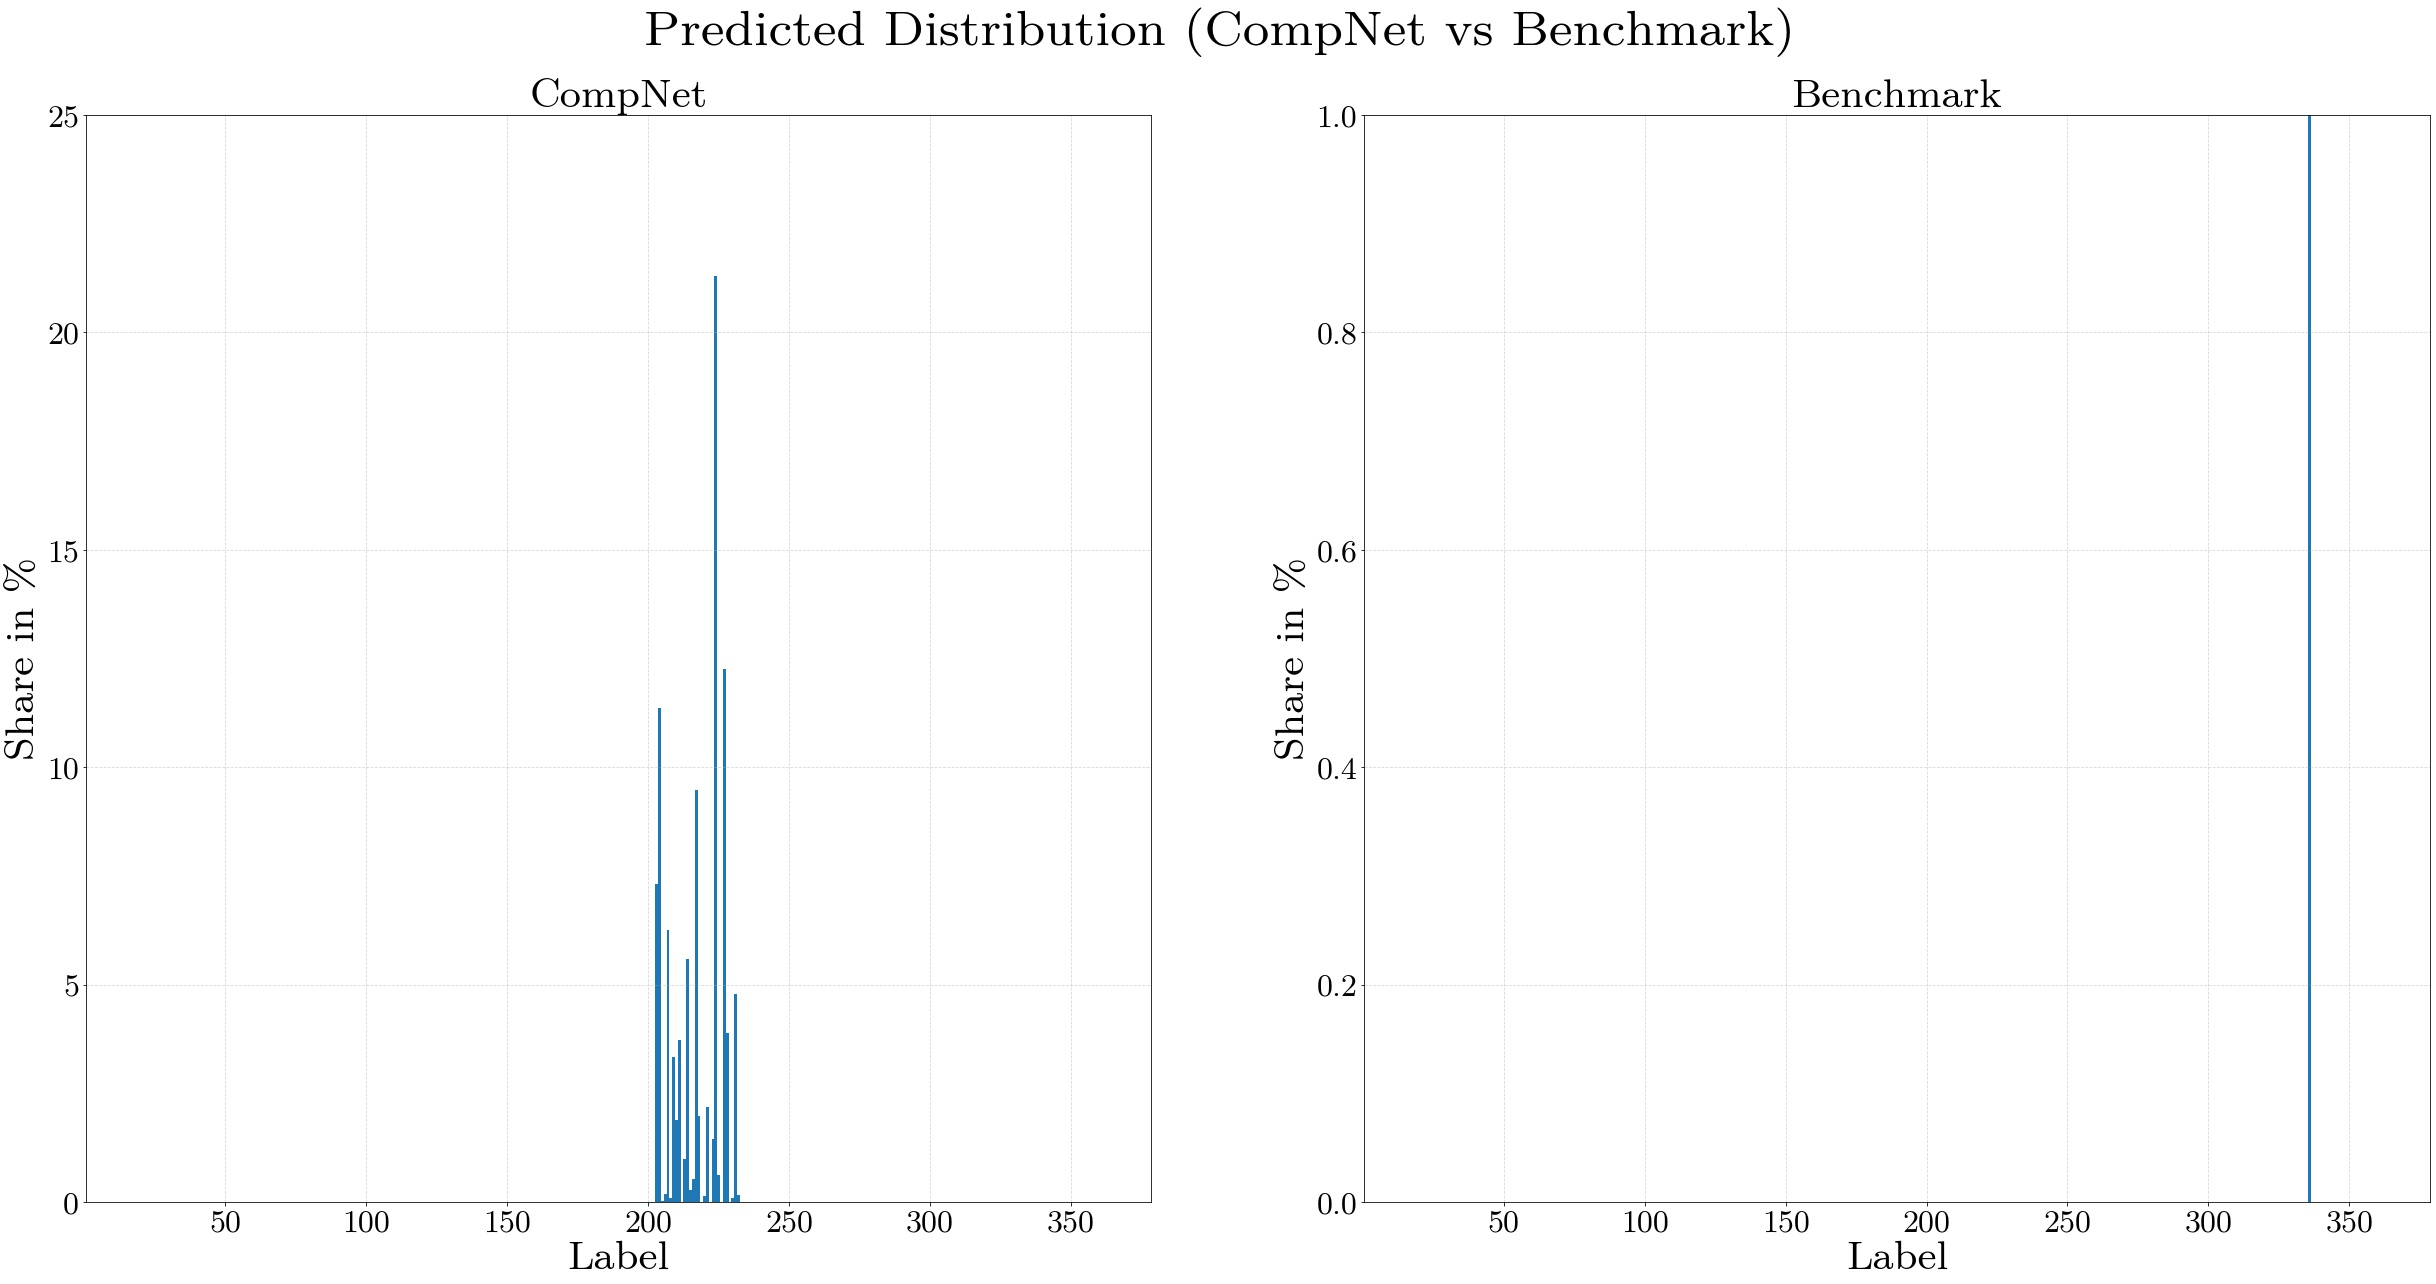
\includegraphics[width=\textwidth, trim=0 -25 0 -25, clip]{thesis/graphics/diagrams/ilsvrc2012/ilsvrc2012_compnet_benchmark_dist_pred_print.jpg}
    \caption{Comparison between the learned predictive distributions of composed and benchmark model.}
    \label{fig:experiments_imagenet_results_predictive_distribution_compnet_benchmark}
\end{figure}

This claim is furthermore supported by the results from the additional testing sequence in which the propagation of the modularization error across hierarchical layers was examined. Figure \ref{fig:experiments_imagenet_results_modelling_error_cat_crossentropy} depicts the categorical crossentropy as a metric for the divergence between ground truth and predictive distribution for each layer respectively. As can be seen, the crossentropy steadily increases for progressing layers, i.\,e.\ the mean value is always higher than the mean of the preceding layer. This qualitatively confirms the hypothesis concerning error propagation in vertical decomposition -- specifically Gating -- formulated in section \ref{sec:compnet_error_propagation}, leading to the intuitive conclusion that the more modules a model consists of, the higher the deviation in comparison to a monolithic model will tendentially be.

\begin{figure}[tb]
    \centering
	    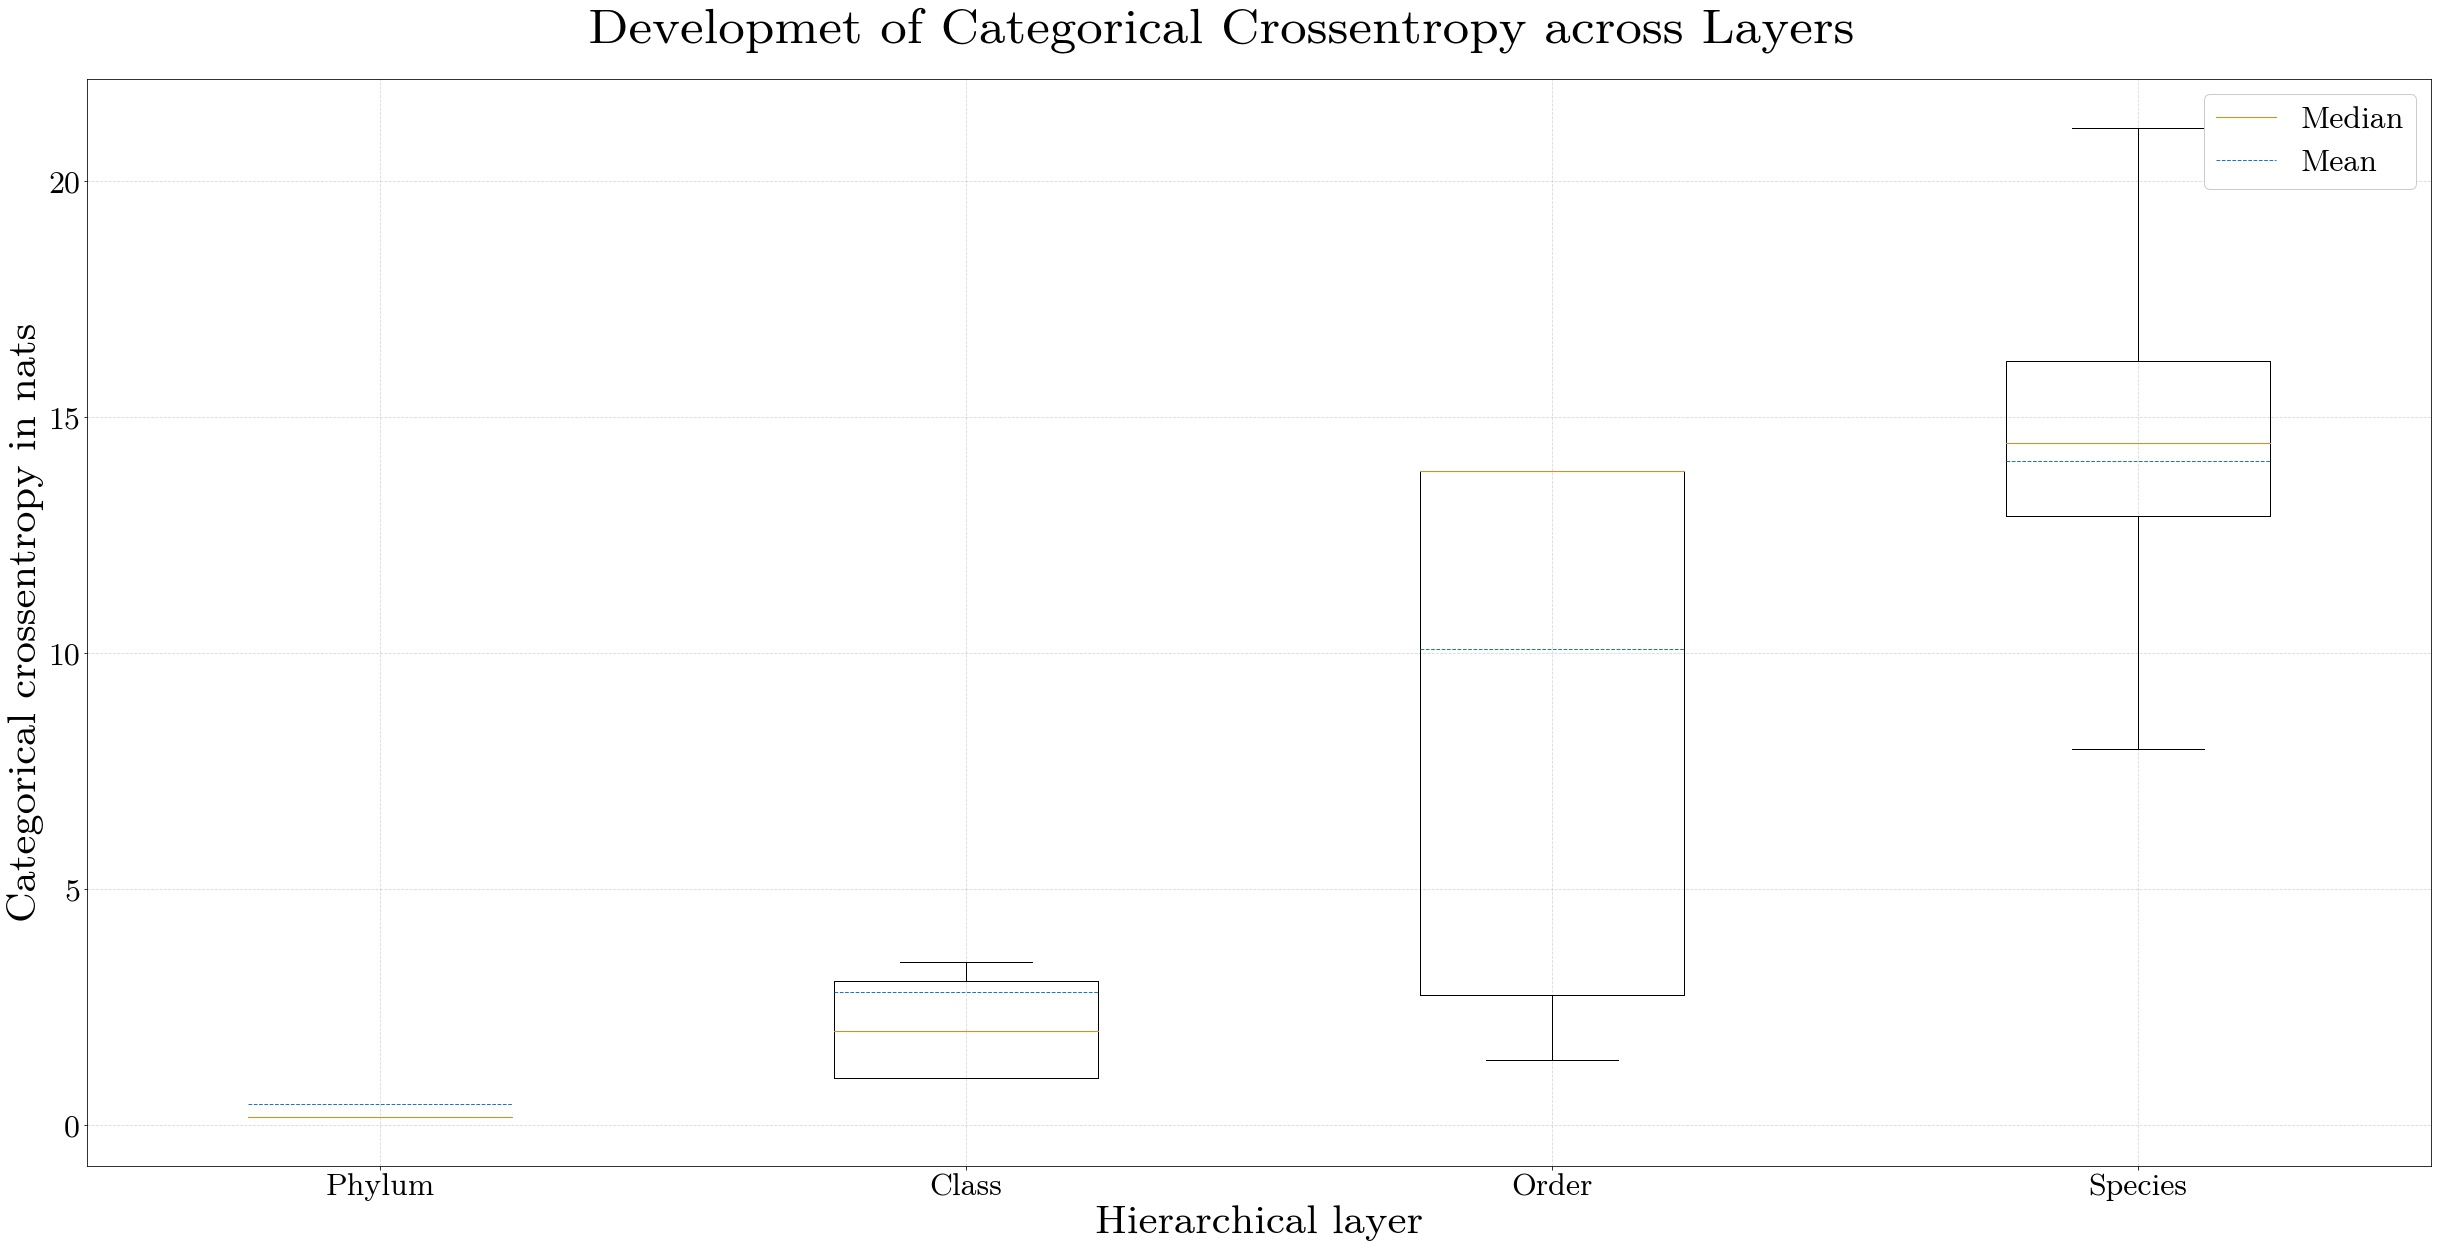
\includegraphics[width=\textwidth, trim=0 -25 0 -25, clip]{thesis/graphics/diagrams/ilsvrc2012/ilsvrc2012_compnet_modelling_error_cat_crossentropy_print.jpg}
    \caption{Development of the categorical crossentropy as a measure for the deviation between the ground truth and the predictive distribution across layers. As can be seen, the metric increases for progressing layers, indicating that the modularization error propagates as discussed in section \ref{sec:compnet_error_propagation}.}
    \label{fig:experiments_imagenet_results_modelling_error_cat_crossentropy}
\end{figure}
               
\subsubsection{Limitations%
               \label{sec:experiments_imagenet_limitations}}

The same limitations as for the first experiment apply. Furthermore, the chosen decomposition of the dataset was selected by arguably arbitrary factors, i.\,e.\ only based on logical deduction and not on empirical evaluation or theoretical foundation. There is no means to ensure that this is the optimum decomposition, i.\,e.\ the one that maximizes the decision boundary margin across the whole label space.

The additional manual effort during the preprocessing of the dataset for preparation of the label space and balancing of the distribution of samples per class that can be seen in this experiment can be said to be a further limitation of the composed approach when compared to a monolithic model from a practical, economic perspective.

The probably gravest limitation of this experiment results from the limited training duration of only five epochs. Consequently, as neither the composed nor the benchmark network have been trained until convergence, comparative inferences are only possible on a qualitative instead of a quantitative basis and should only be generalized with caution. All the more so since, as stated before, such a training snapshot inherently biases the results in favor of the composed network as smaller models generally converge faster than bigger networks. Thus -- even though this also serves to practically demonstrate one of the key advantages of the modularized approach -- the composed model as a whole will always be relatively closer to convergence after the same amount of epochs. This effect diminishes with increasing training time when adversary aspects such as modularization errors and reduced modeling capacity of the individual submodules start to show impact. But especially in the early training process that is observed here, the composed network is advantaged.

Lastly, with regard to the results concerning modeling error propagation, it is to be taken into consideration that only Gating as inter-layer interface was considered here; no statement was made regarding the other kinds of connectivity listed in section \ref{sec:compnet_modularization_types}.

\subsection{Evaluation of uncertainty%
            \label{sec:experiments_uncertainty}}
            
\subsubsection{Overview%
               \label{sec:experiments_uncertainty_overview}}
               
The third experiment served to assess the effect of modularization with regard to predictive robustness. Following the basic procedure of \cite{Ovadia2019-zt}, the performance of a hierarchically composed and a monolithic reference model was evaluated and compared on distributionally shifted and OOD (Out-Of-Distribution) testing data. Brier Score according to \cite{Brier1950-jb}, confidence, categorical accuracy and predictive entropy were measured to gain insights into how modularization affects model calibration and how increasing distributional dataset shift impacts the predictive behavior of composed networks. The latter is of particular importance as the safety margin constitutes a major decision factor for a model's applicability in many real-world scenarios.
               
\subsubsection{Datasets%
               \label{sec:experiments_uncertainty_dataset}}

\begin{figure}[tb]
    \centering
	    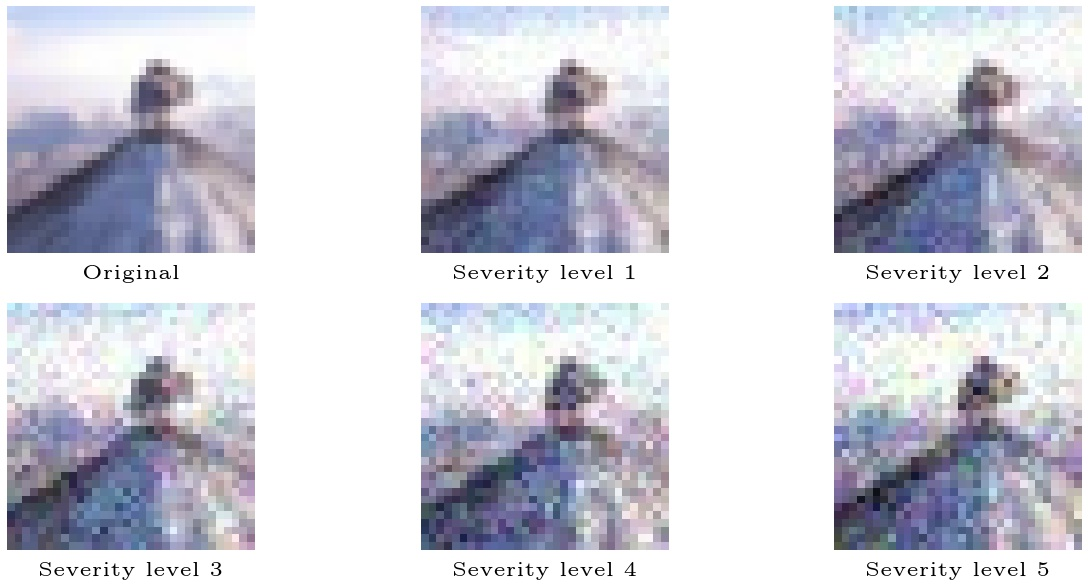
\includegraphics[width=\textwidth]{thesis/graphics/images/cifar100_c_severities_gaussian_noise.jpg}
    \caption{Gaussian noise applied to a sample image with different degrees of intensity. As can be seen, the distributional shift from the original image increases with higher severity levels.}
    \label{fig:experiments_uncertainty_severities_gaussian_noise}
\end{figure}

In this experiment, three different datasets were employed. Similar to the first experiment, training and evaluation were performed utilizing the CIFAR100 dataset (cf.\ section \ref{sec:experiments_cifar100_dataset}). During testing, the CIFAR100-C and the CIFAR10 datasets were used to model distributionally shifted and OOD data respectively.

CIFAR100-C is based on CIFAR100 and was established as part of the work of \cite{Hendrycks2019-gi}. It extends the original dataset by applying 19 different kinds of corruptions commonly found in photographs with five varying severity grades to the image base. It consists of 950,000 records in total (19 corruptions $\cdot$ 5 severities $\cdot$ 10,000 samples in the testing set) and is thought mainly for testing resp.\ evaluating the robustness of object recognition models. The label structure is equivalent to the base dataset. Examples of the different corruptions are depicted in figures \ref{fig:experiments_uncertainty_severities_gaussian_noise} and \ref{fig:experiments_uncertainty_sample_images}.

The CIFAR10 dataset was initially established by \cite{Krizhevsky2009-wt} and is -- similar to CIFAR100 -- a subset of the tiny image dataset. It consists of 60,000 hand-labeled 32x32 pixel color (RGB) images (50,000 records for training and 10,000 for testing) of 10 different categories. Since these categories are mutually exclusive with the CIFAR100 label space while the basic structure of both datasets is similar, we employed the CIFAR10 testing set to model OOD samples, i.\,e.\ examples of classes that the network has not seen during training.

\subsubsection{Models%
               \label{sec:experiments_uncertainty_models}}
               
The composed network as well as the benchmark model used in this experiment adhered to the same structure as described in section \ref{sec:experiments_cifar100_models}.

\pagebreak

\begin{figure}[htb]
    \centering
	    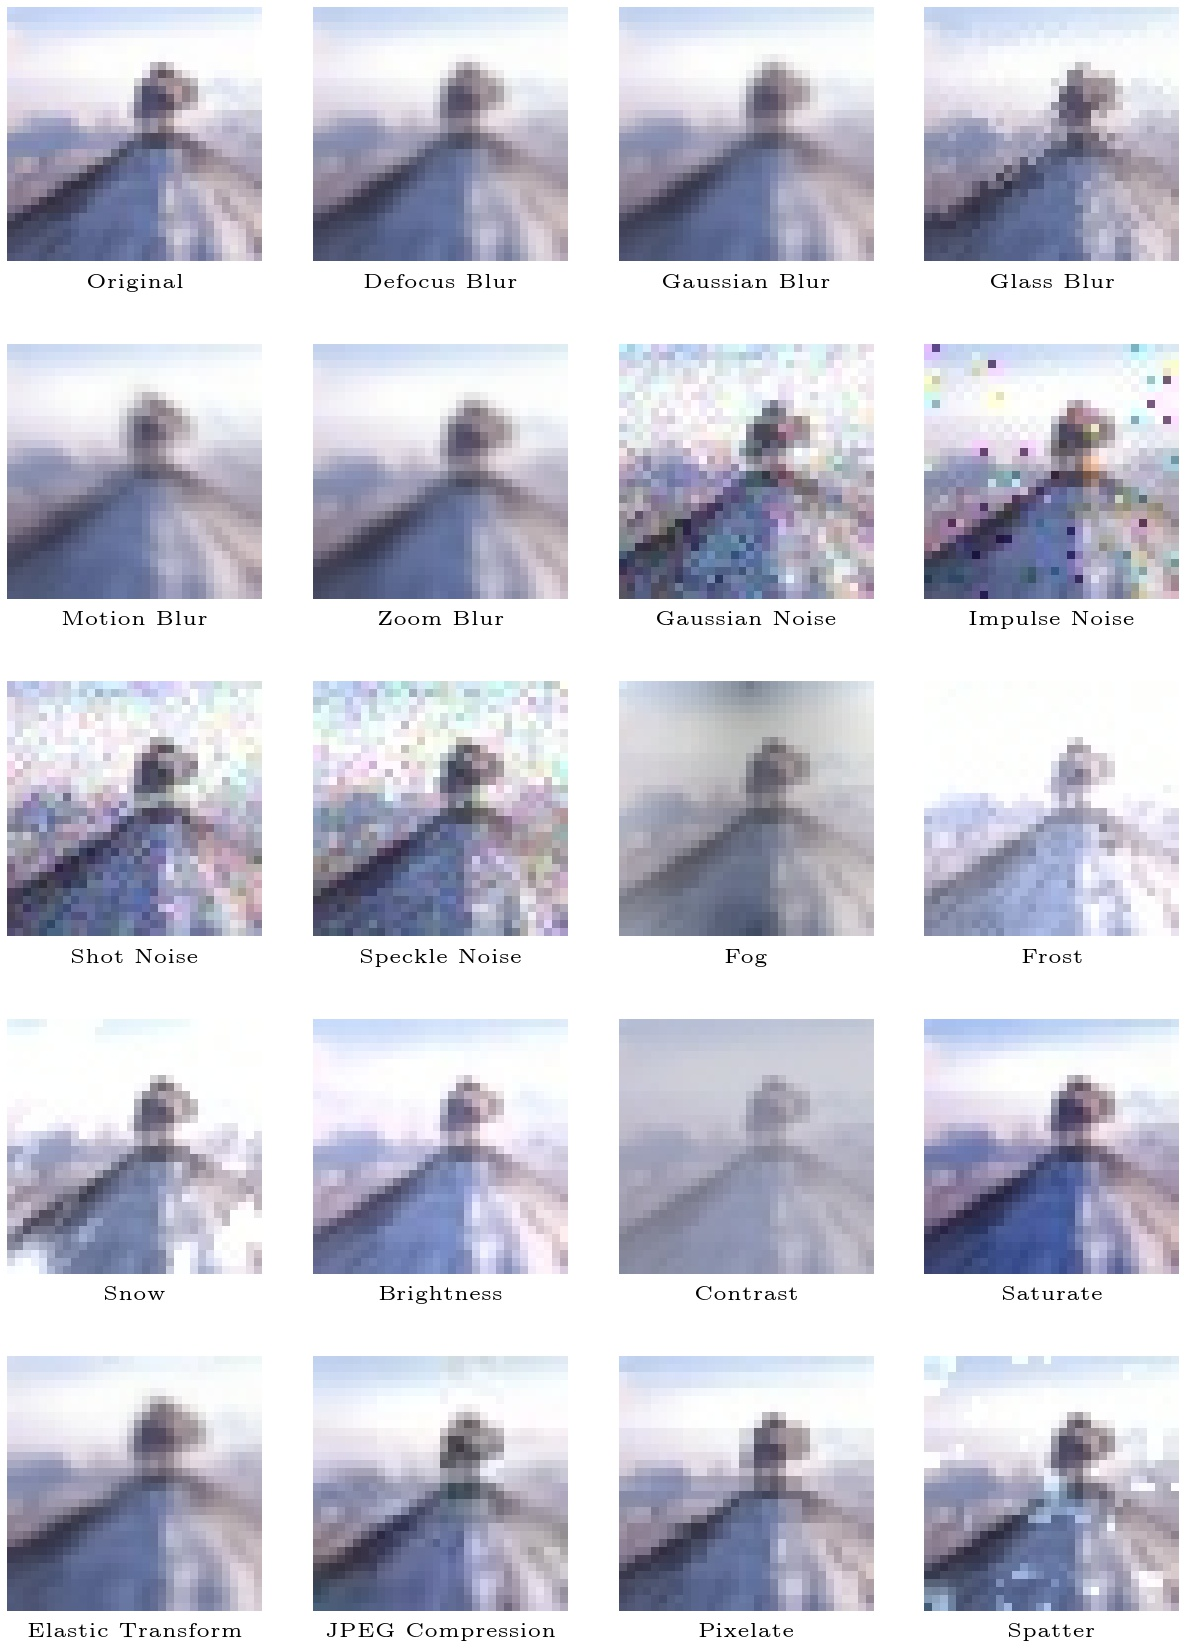
\includegraphics[width=\textwidth]{thesis/graphics/images/cifar100_c_sample_images.jpg}
    \caption{Exemplary overview of the different corruption types of the CIFAR100-C dataset for severity level 3 out of 5.}
    \label{fig:experiments_uncertainty_sample_images}
\end{figure}

\clearpage

\subsubsection{Training%
               \label{sec:experiments_uncertainty_training}}
               
The preprocessing procedure as well as the training itself were similar to the first experiment (cf.\ section \ref{sec:experiments_cifar100_training}). No differing or additional steps were employed.
               
\subsubsection{Testing%
               \label{sec:experiments_uncertainty_testing}}

Preprocessing during testing was done independently of the dataset. Similar to the first experiment, images were one-hot encoded and repeated once with the duplicate being flipped along the horizontal axis. Five 28x28 pixel crops were subsequently extracted at all four corner positions as well as the center of each record. Batch size was set to 10 records per batch so that each batch represented exactly one source image. Predictions were then calculated by averaging the scores of all images per batch.

Again, in the case of the composed network, the batches were first evaluated on the coarse-layer model. Afterwards, they were fed to the fine-layer module with the maximum coarse-layer score. The fine-layer predictions were then interpreted as the final prediction of the network.

During the evaluation on the distributionally shifted data, the confidence, predictive accuracy, Brier Score and predictive entropy were measured. The results were subsequently sorted and grouped together by severity levels of the different kinds of corruption of the CIFAR100-C dataset to obtain a statement concerning the model's robustness independent of the individual error types.

As for the OOD data, since the label space of the CIFAR100 and the CIFAR10 datasets are mutually exclusive, there is no ground truth in the conventional sense. Consequently, only the confidence and the predictive entropy could be measured.

\subsubsection{Results \& Discussion%
               \label{sec:experiments_uncertainty_results}}

\begin{figure}[tb]
    \centering
	    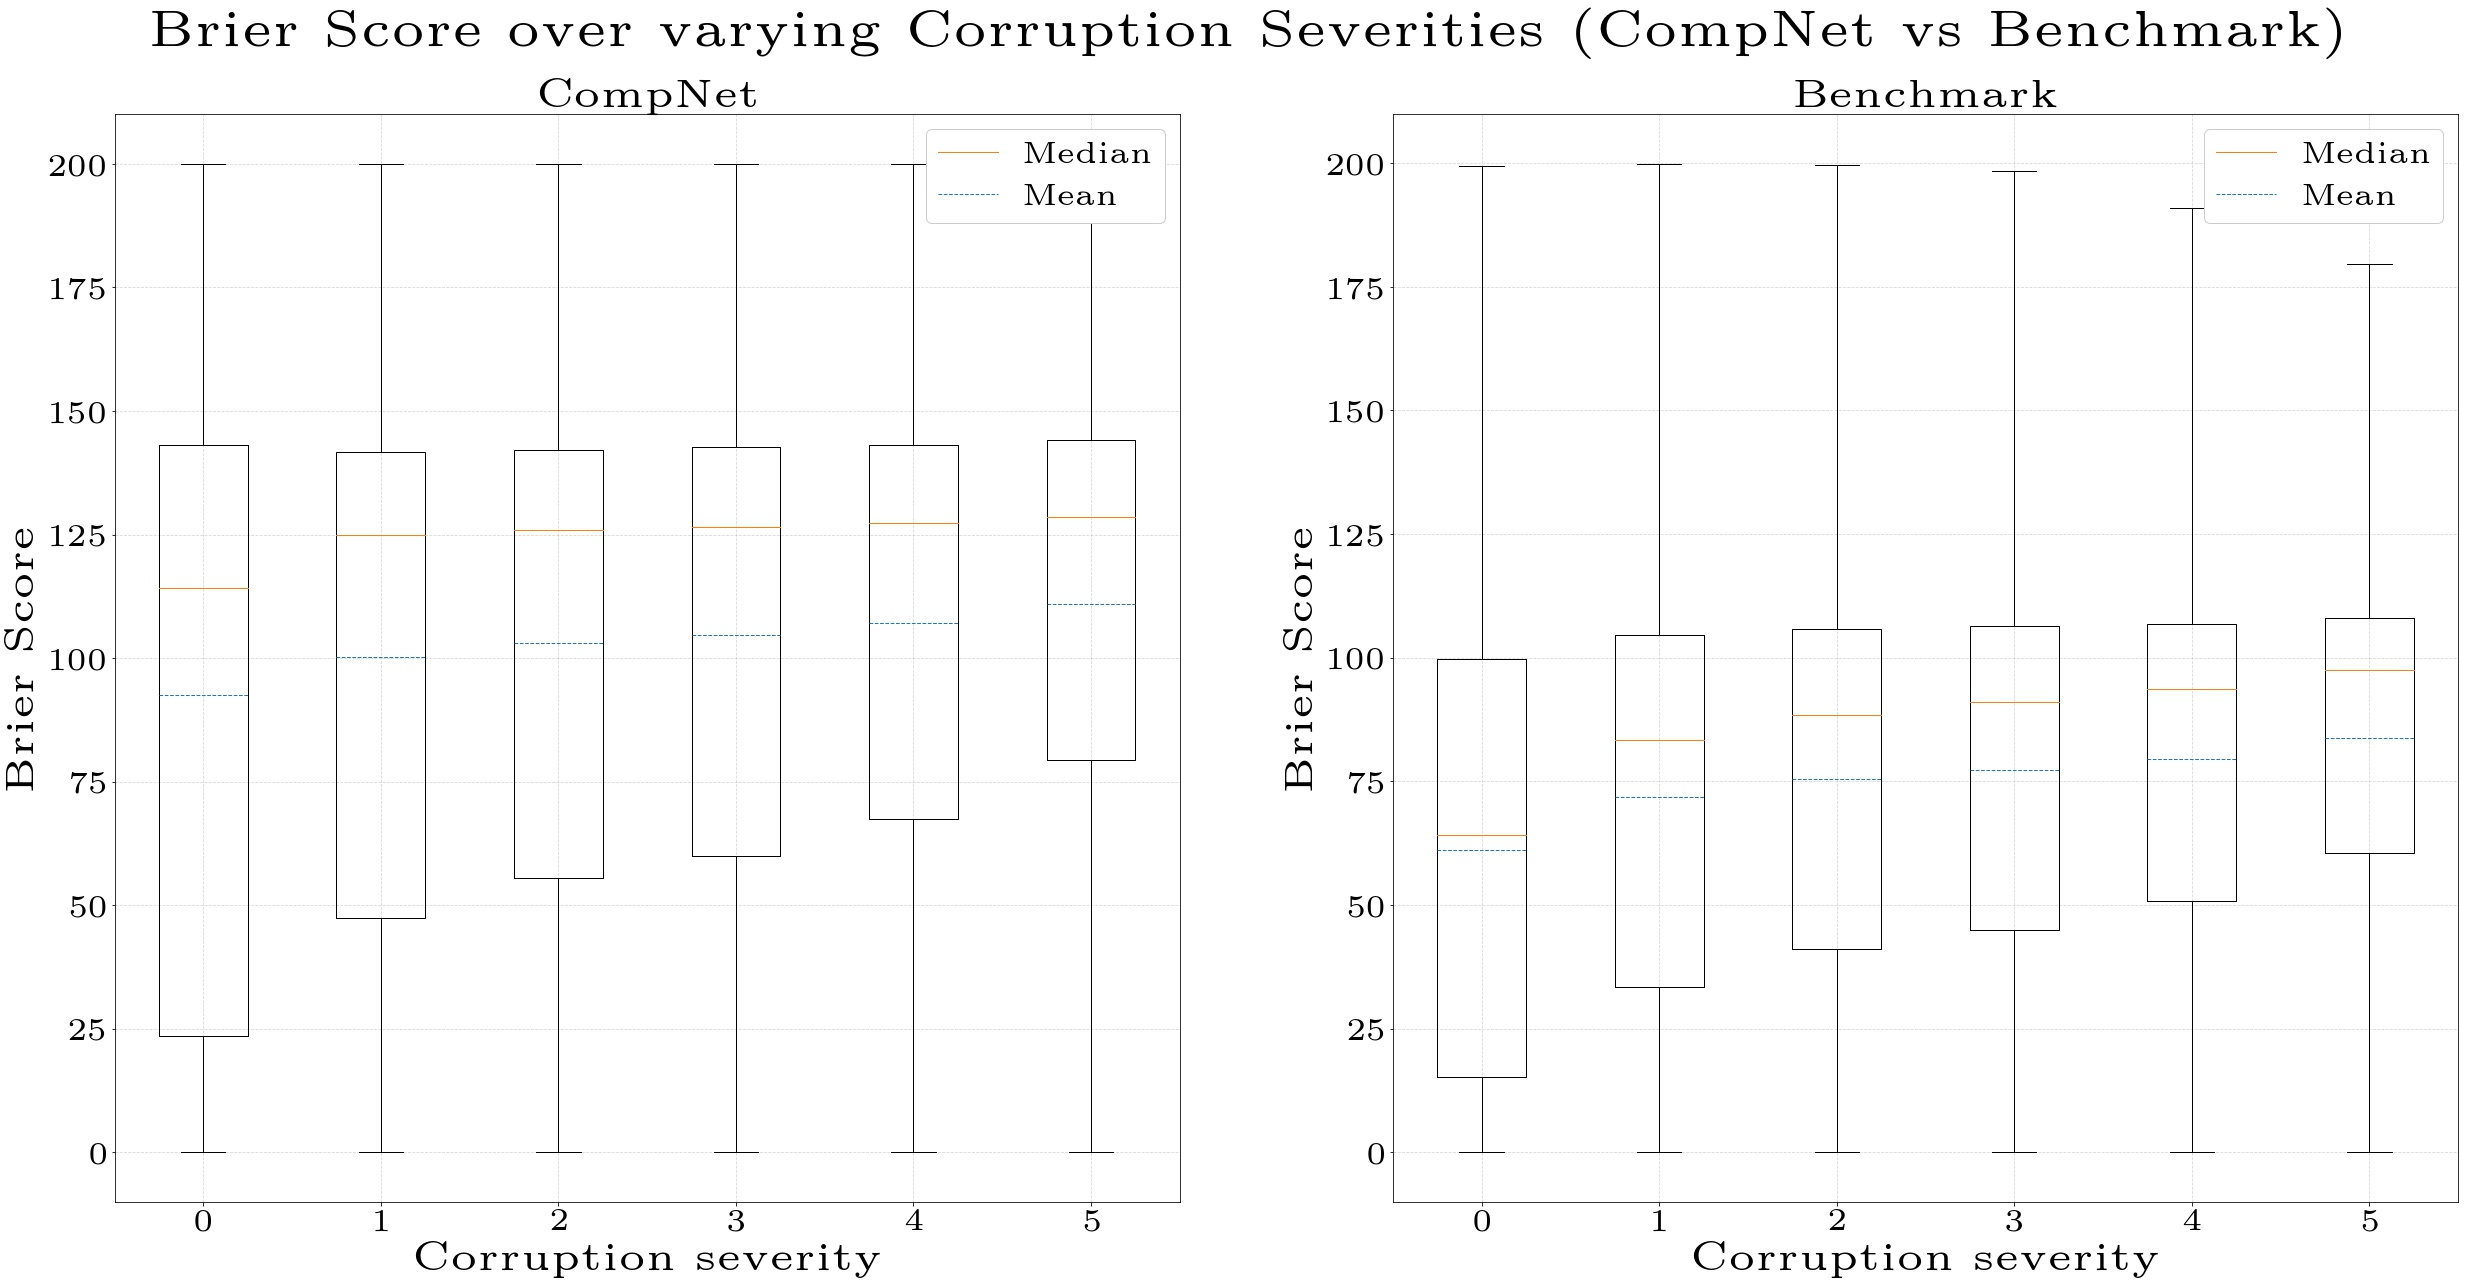
\includegraphics[width=\textwidth, trim=0 -25 0 -25, clip]{thesis/graphics/diagrams/uncertainty/uncertainty_compnet_benchmark_ds_brier_score_print.jpg}
    \caption{Development of the Brier Score for increasing severity levels. While the score of the composite model is slightly higher, the qualitative change with growing distributional shift is similar, indicating that modular networks are not more susceptible than conventional models.}
    \label{fig:experiments_uncertainty_results_ds_brier_score}
\end{figure}

On the distributionally shifted dataset, the average categorical accuracy of the composed network ranges from 35.26\% on the uncorrupted to 20.69\% on the most severely corrupted data; the accuracy of the monolithic reference model steadily declines from 53.19\% to 30.29\%. Similarly, the average confidence decreases from 64.53\% to 57.87\% resp.\ 48.18\% to 36.42\%. However, the Brier Score as a measure of calibration increases from 0.93 to 1.11 for the composite and 0.61 to 0.83 for the benchmark model (cf.\ figure \ref{fig:experiments_uncertainty_results_ds_brier_score}), indicating that both models lose their calibration with growing distributional shift. As shown in figure \ref{fig:experiments_uncertainty_results_ds_confidence_accuracy}, this results in an increasing deviation between the models' confidence in their predictions and the actual accuracy. This goes along with a similarly increasing entropy from 0.88 to 1.04 nats resp.\ 1.99 to 2.48 nats, which shows that, despite the over-confidence of the models in their predictions, the growing uncertainty with higher corruption severities is nevertheless also being reflected.

These results are in line with the overall slightly worse performance of the composed in comparison to the benchmark network reported in section \ref{sec:experiments_cifar100_results}. Especially the generally higher Brier Score and lower entropy of the composed model are explainable by the fact that the final prediction is sampled from the label space of a single submodule instead of from the whole fine-layer label space. Thus, when measured over the latter, the predictions of the former inherently appear to be much more narrow-banded than those of the monolithic network.

However interestingly, while the absolute offset in the results can be interpreted as a direct consequence of the error inferred by the modularization, the qualitative behavior of both models is almost completely identical. Figure \ref{fig:experiments_uncertainty_results_ds_metrics_development} depict the relative development of the different metrics with increasing corruption severity grades. As can be seen, the rate with which the performance decreases is -- with minor deviations -- highly correlated. The slightly higher absolute deviation in the development of the confidence can again be attributed to the more narrower-banded predictions of the composite network.

The results on the OOD set match those of the distributionally shifted data. The confidence further decreases to 56.39\% for the composed resp.\ 31.52\% for the monolithic network. Similarly, the average predictive entropy increases to 1.05 and 2.64 nats. This is in line with the previous observations and continues the trend of a proportional development of both models.

\begin{figure}[tb]
    \centering
	    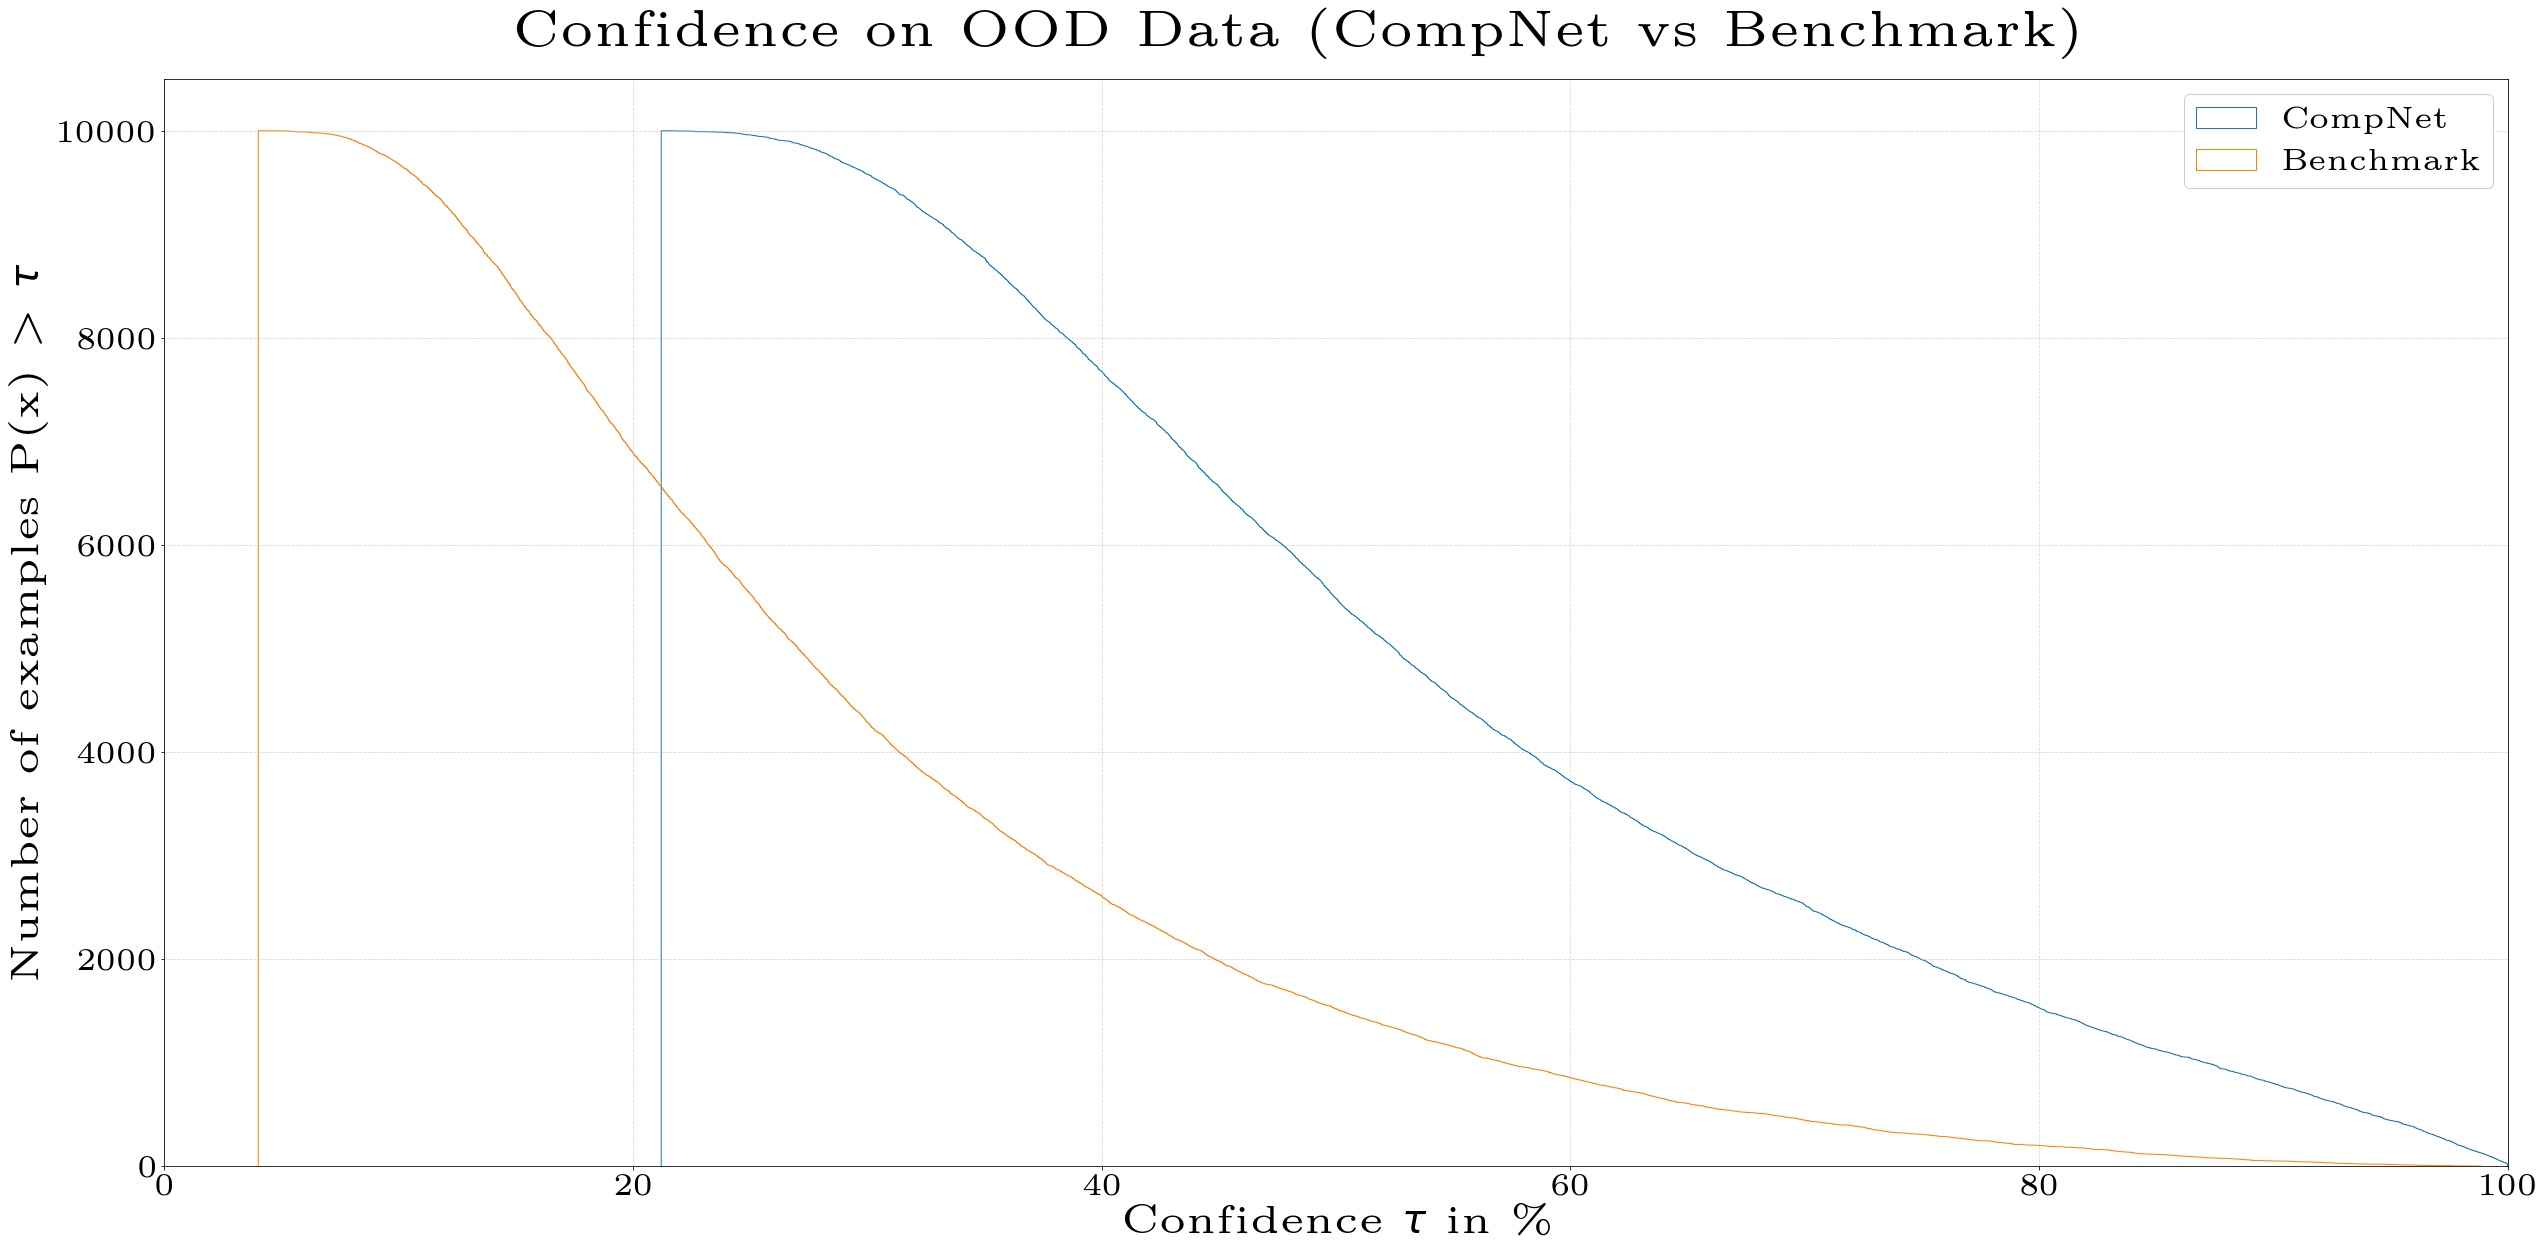
\includegraphics[width=\textwidth, trim=0 0 0 -25, clip]{thesis/graphics/diagrams/uncertainty/uncertainty_compnet_benchmark_ood_confidence_print.jpg}
	    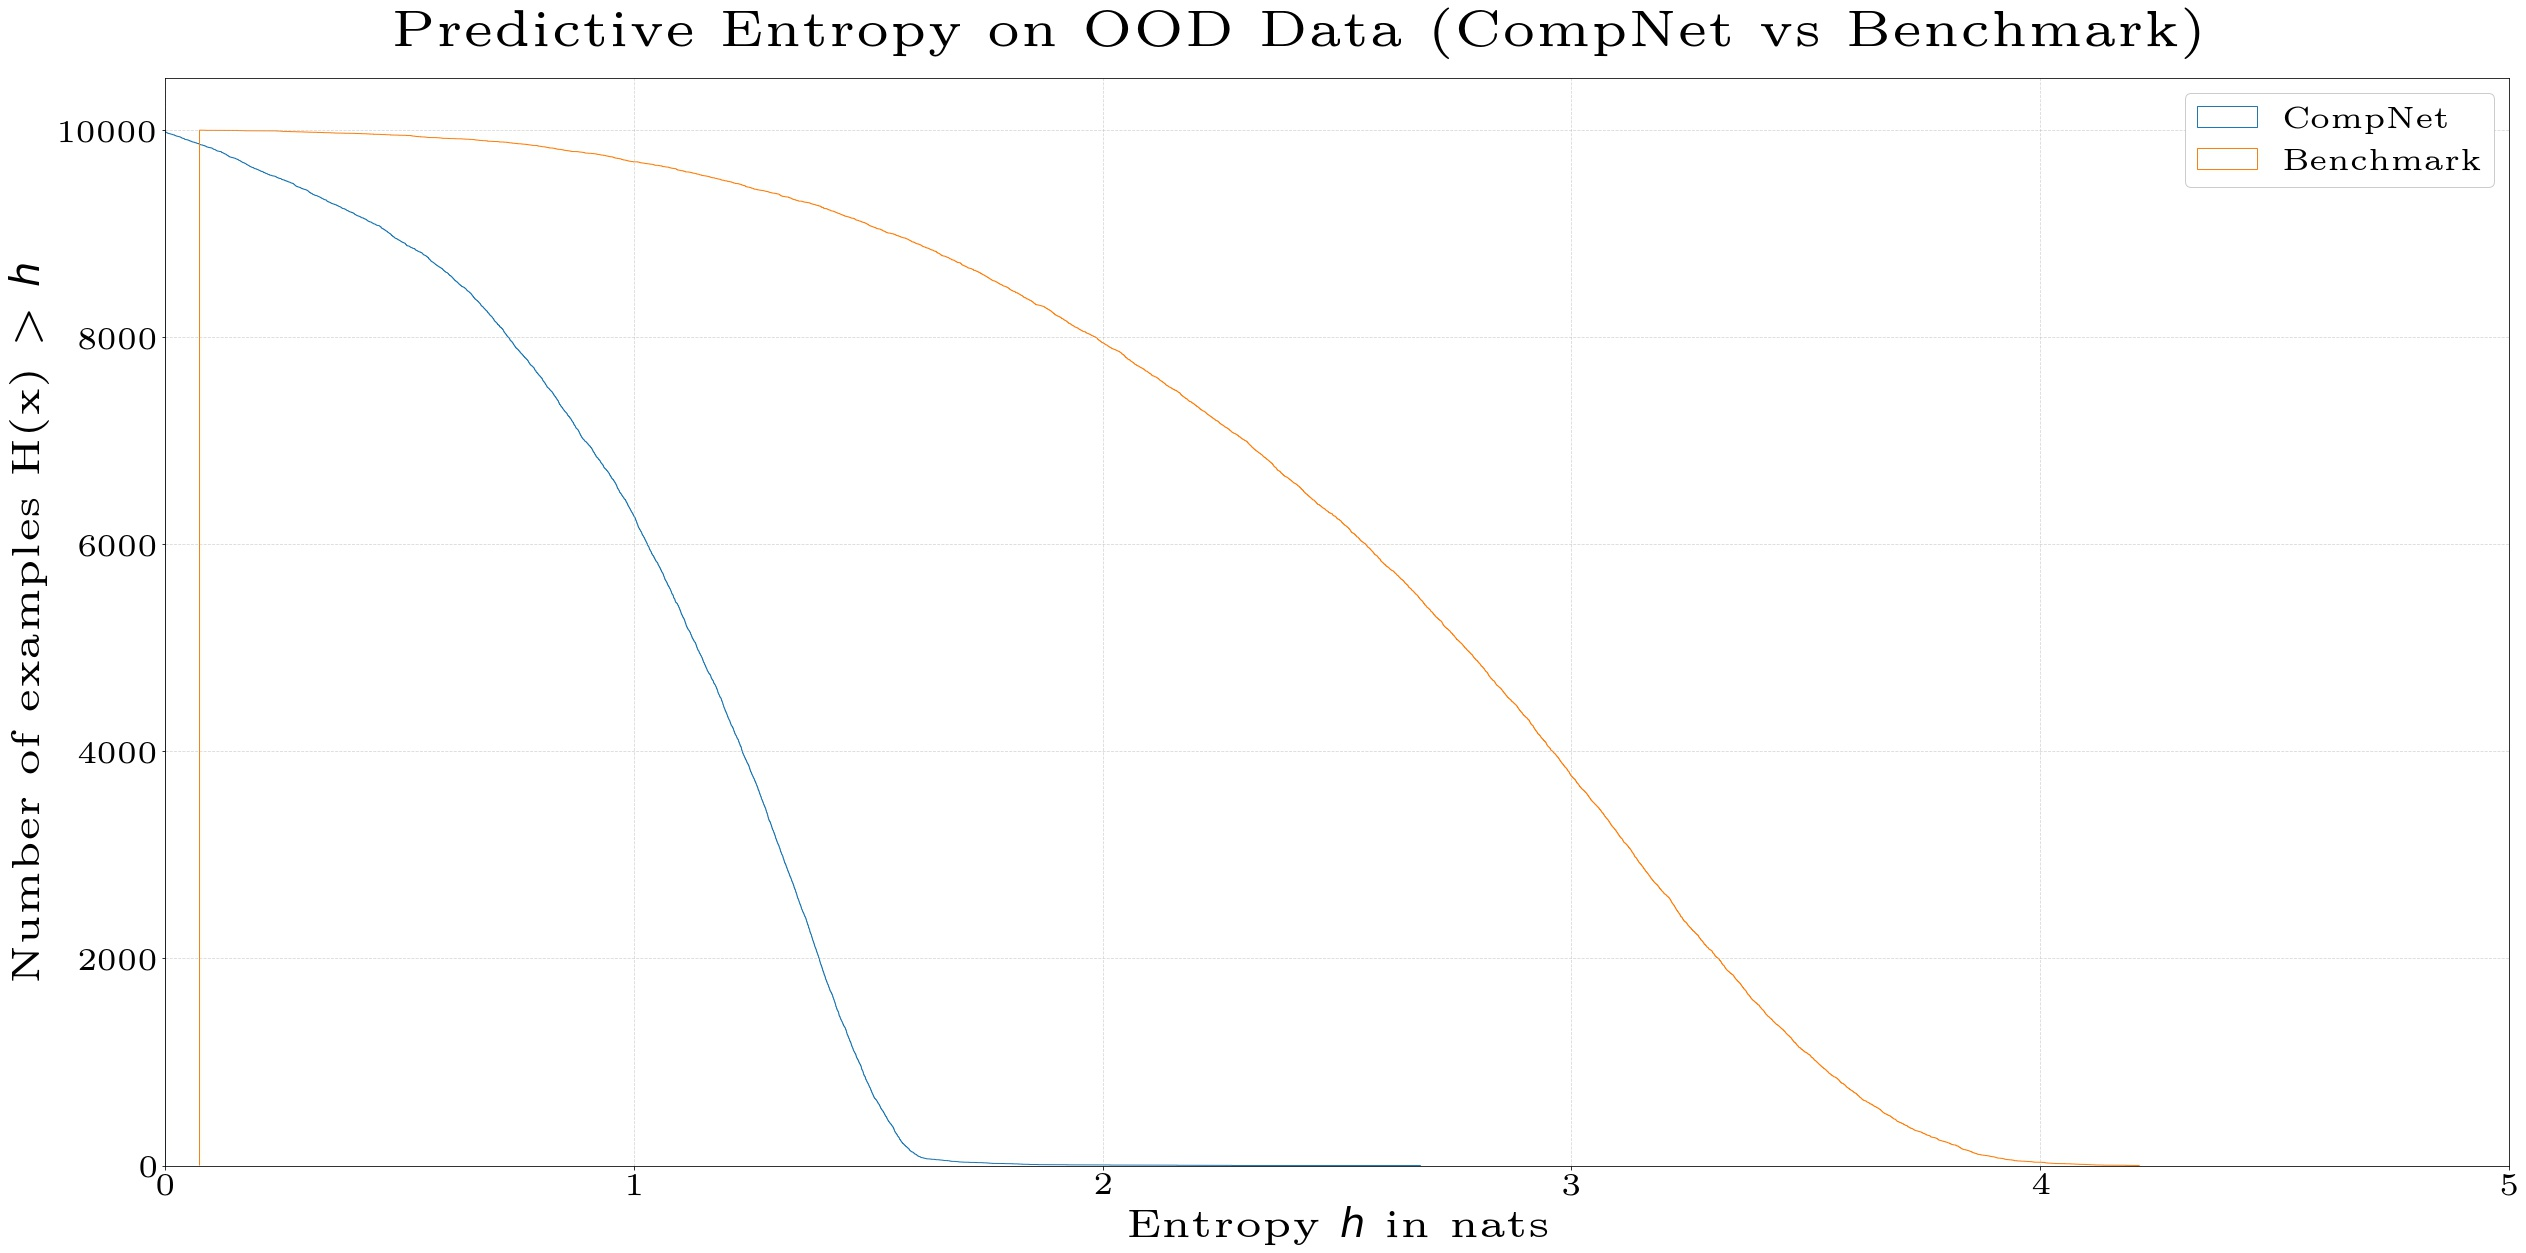
\includegraphics[width=\textwidth, trim=0 -25 0 0, clip]{thesis/graphics/diagrams/uncertainty/uncertainty_compnet_benchmark_ood_pred_entropy_print.jpg}
    \caption{Confidence and predictive entropy on the OOD dataset. The results are in line with the findings on the distributionally shifted data.}
    \label{fig:experiments_uncertainty_results_ood_confidence_pred_entropy}
\end{figure}

It can be concluded that the composite model is not less robust than its non-modularized counterpart. Even without further calibration measures, both networks reflect the continuous distributional data shift in their respective predictions. Furthermore, these results suggest that while the modularization introduces an absolute error that impacts the performance of the model, it does not significantly affect the overall behavior.
               
\subsubsection{Limitations%
               \label{sec:experiments_uncertainty_limitations}}
            
Limitations are similar to the first two experiments. Mainly due to the aforementioned restrictions regarding the available computing power, we were only able to assess the impacts of modularization on the model robustness for a fixed layer depth, i.\,e.\ we did not evaluate the effect of additional layers. Thus the results are of qualitative character only and generalization to other model structures should be done with caution. The same applies to the inter-module connectivity mechanisms employed for the composed model in this experiment. Solely Layering, more specifically Gating, was used for modularization; Chaining and Aggregation were not considered. Especially concerning the observed behavioral retention of the composed model it is thus questionable whether this result can be generalized to other forms of decomposition as well.

Additionally, even though the primary goal was to assess the general impact of distributional shift on the robustness of composed models, no further distinction between different kinds of corruptions was made. In practice, many technical applications struggle only with a limited spectrum of error types and not with all at once. Consequently, it might be of interest to know if a specific model is e.\,g.\ more resistant to noise than to blur effects.

\pagebreak

\begin{figure}[htb]
    \centering
	    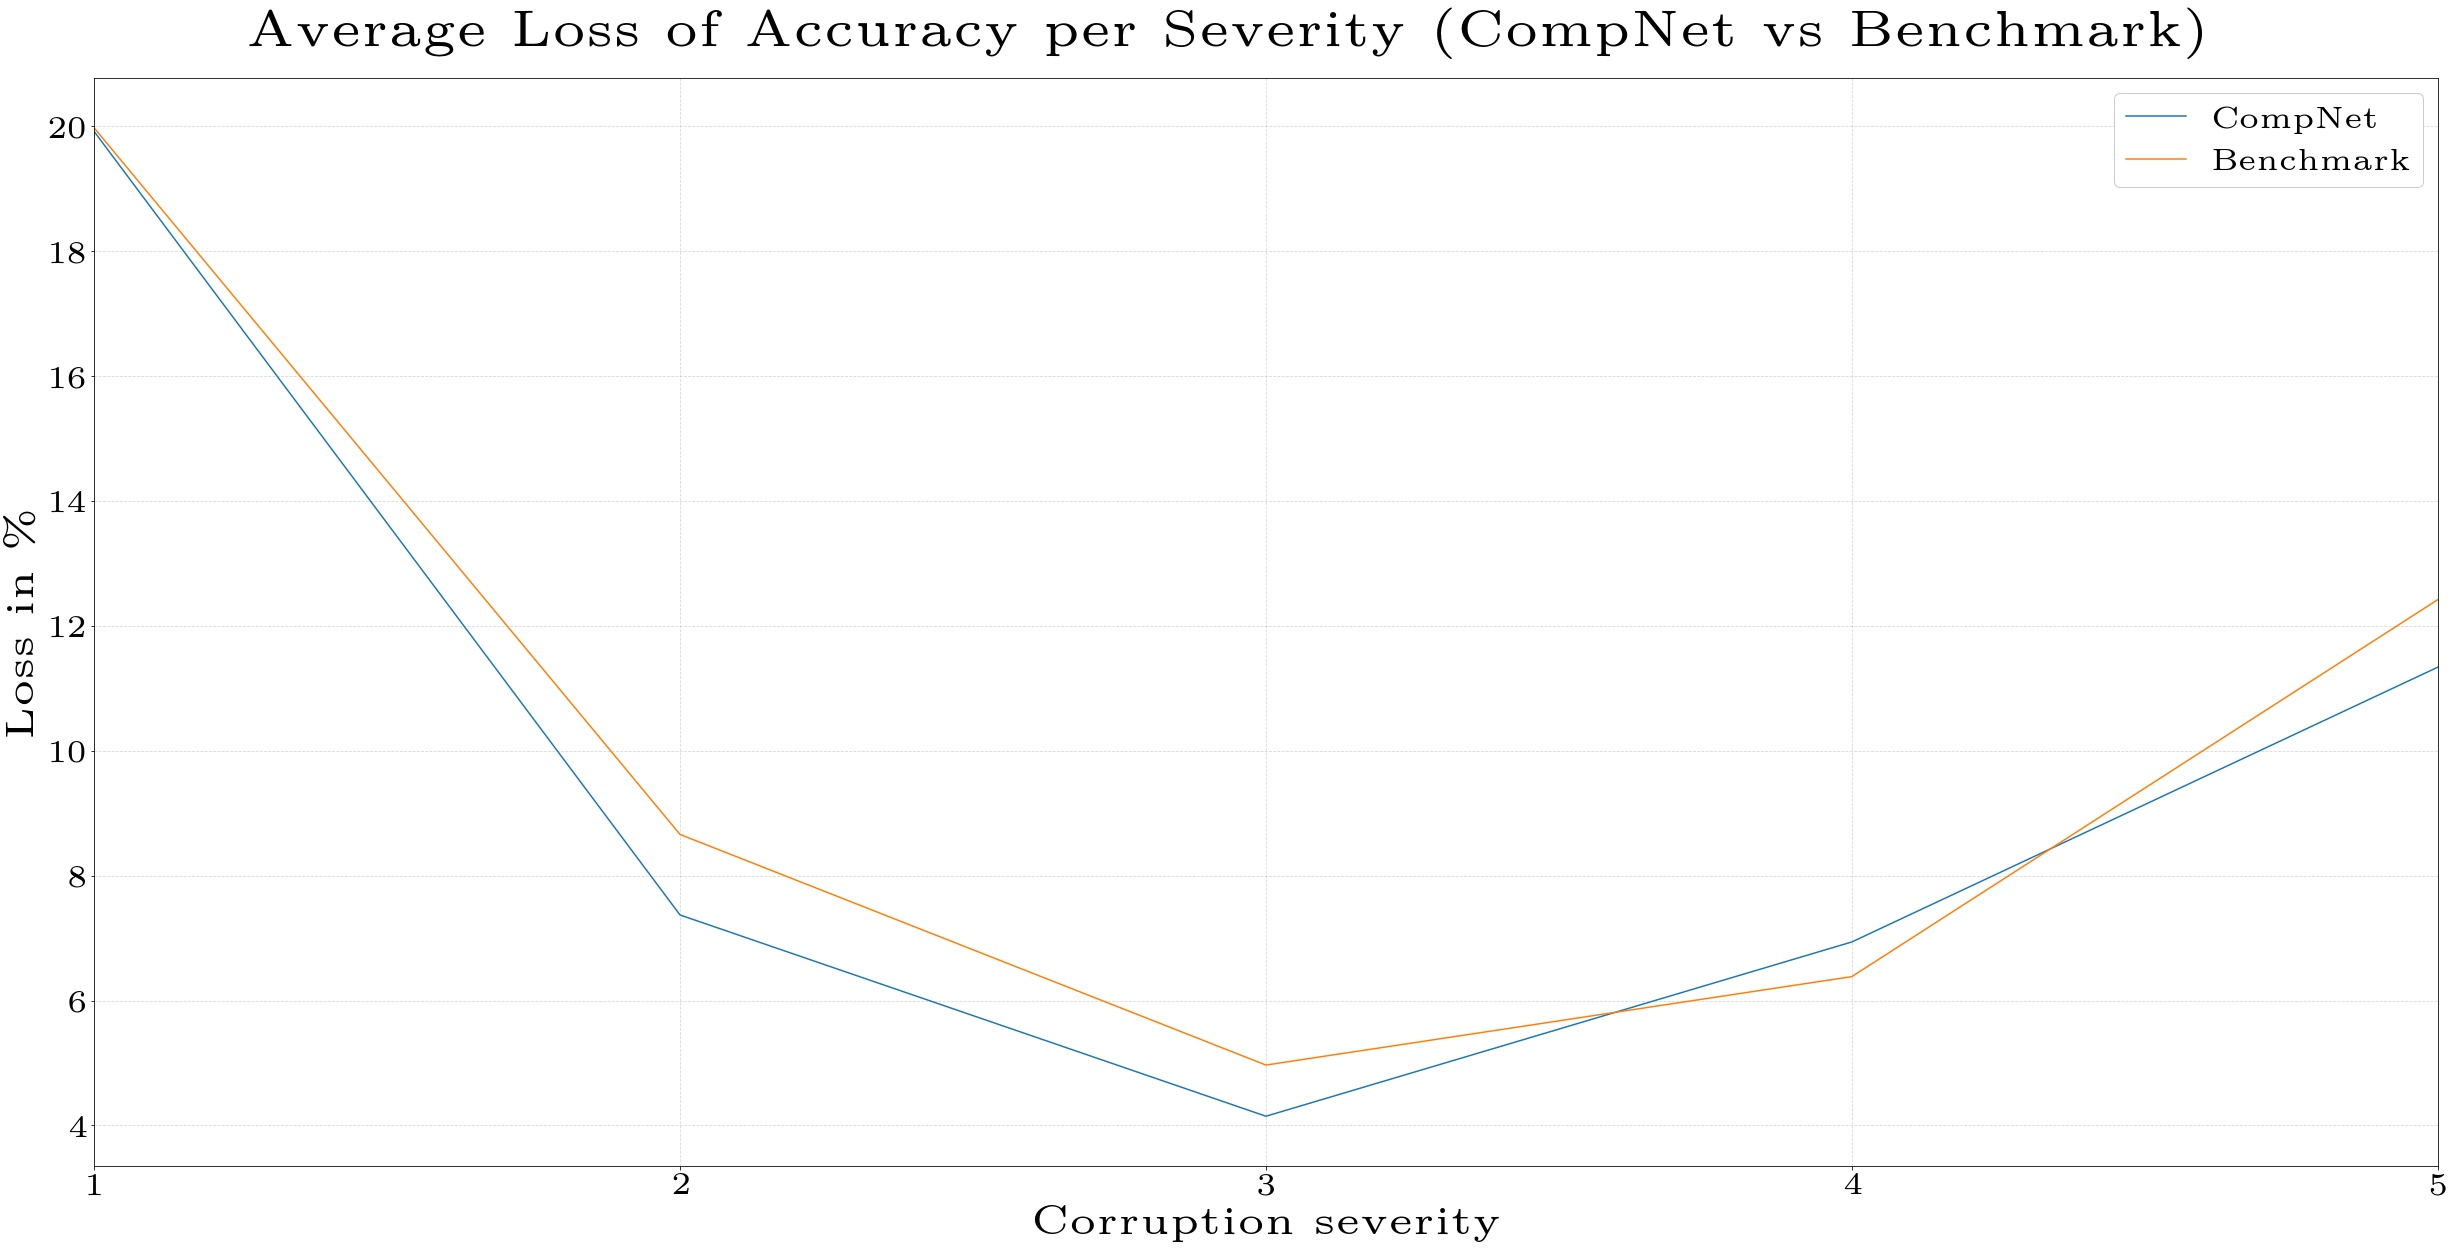
\includegraphics[width=\textwidth]{thesis/graphics/diagrams/uncertainty/uncertainty_compnet_benchmark_ds_cat_acc_loss_print.jpg}
	    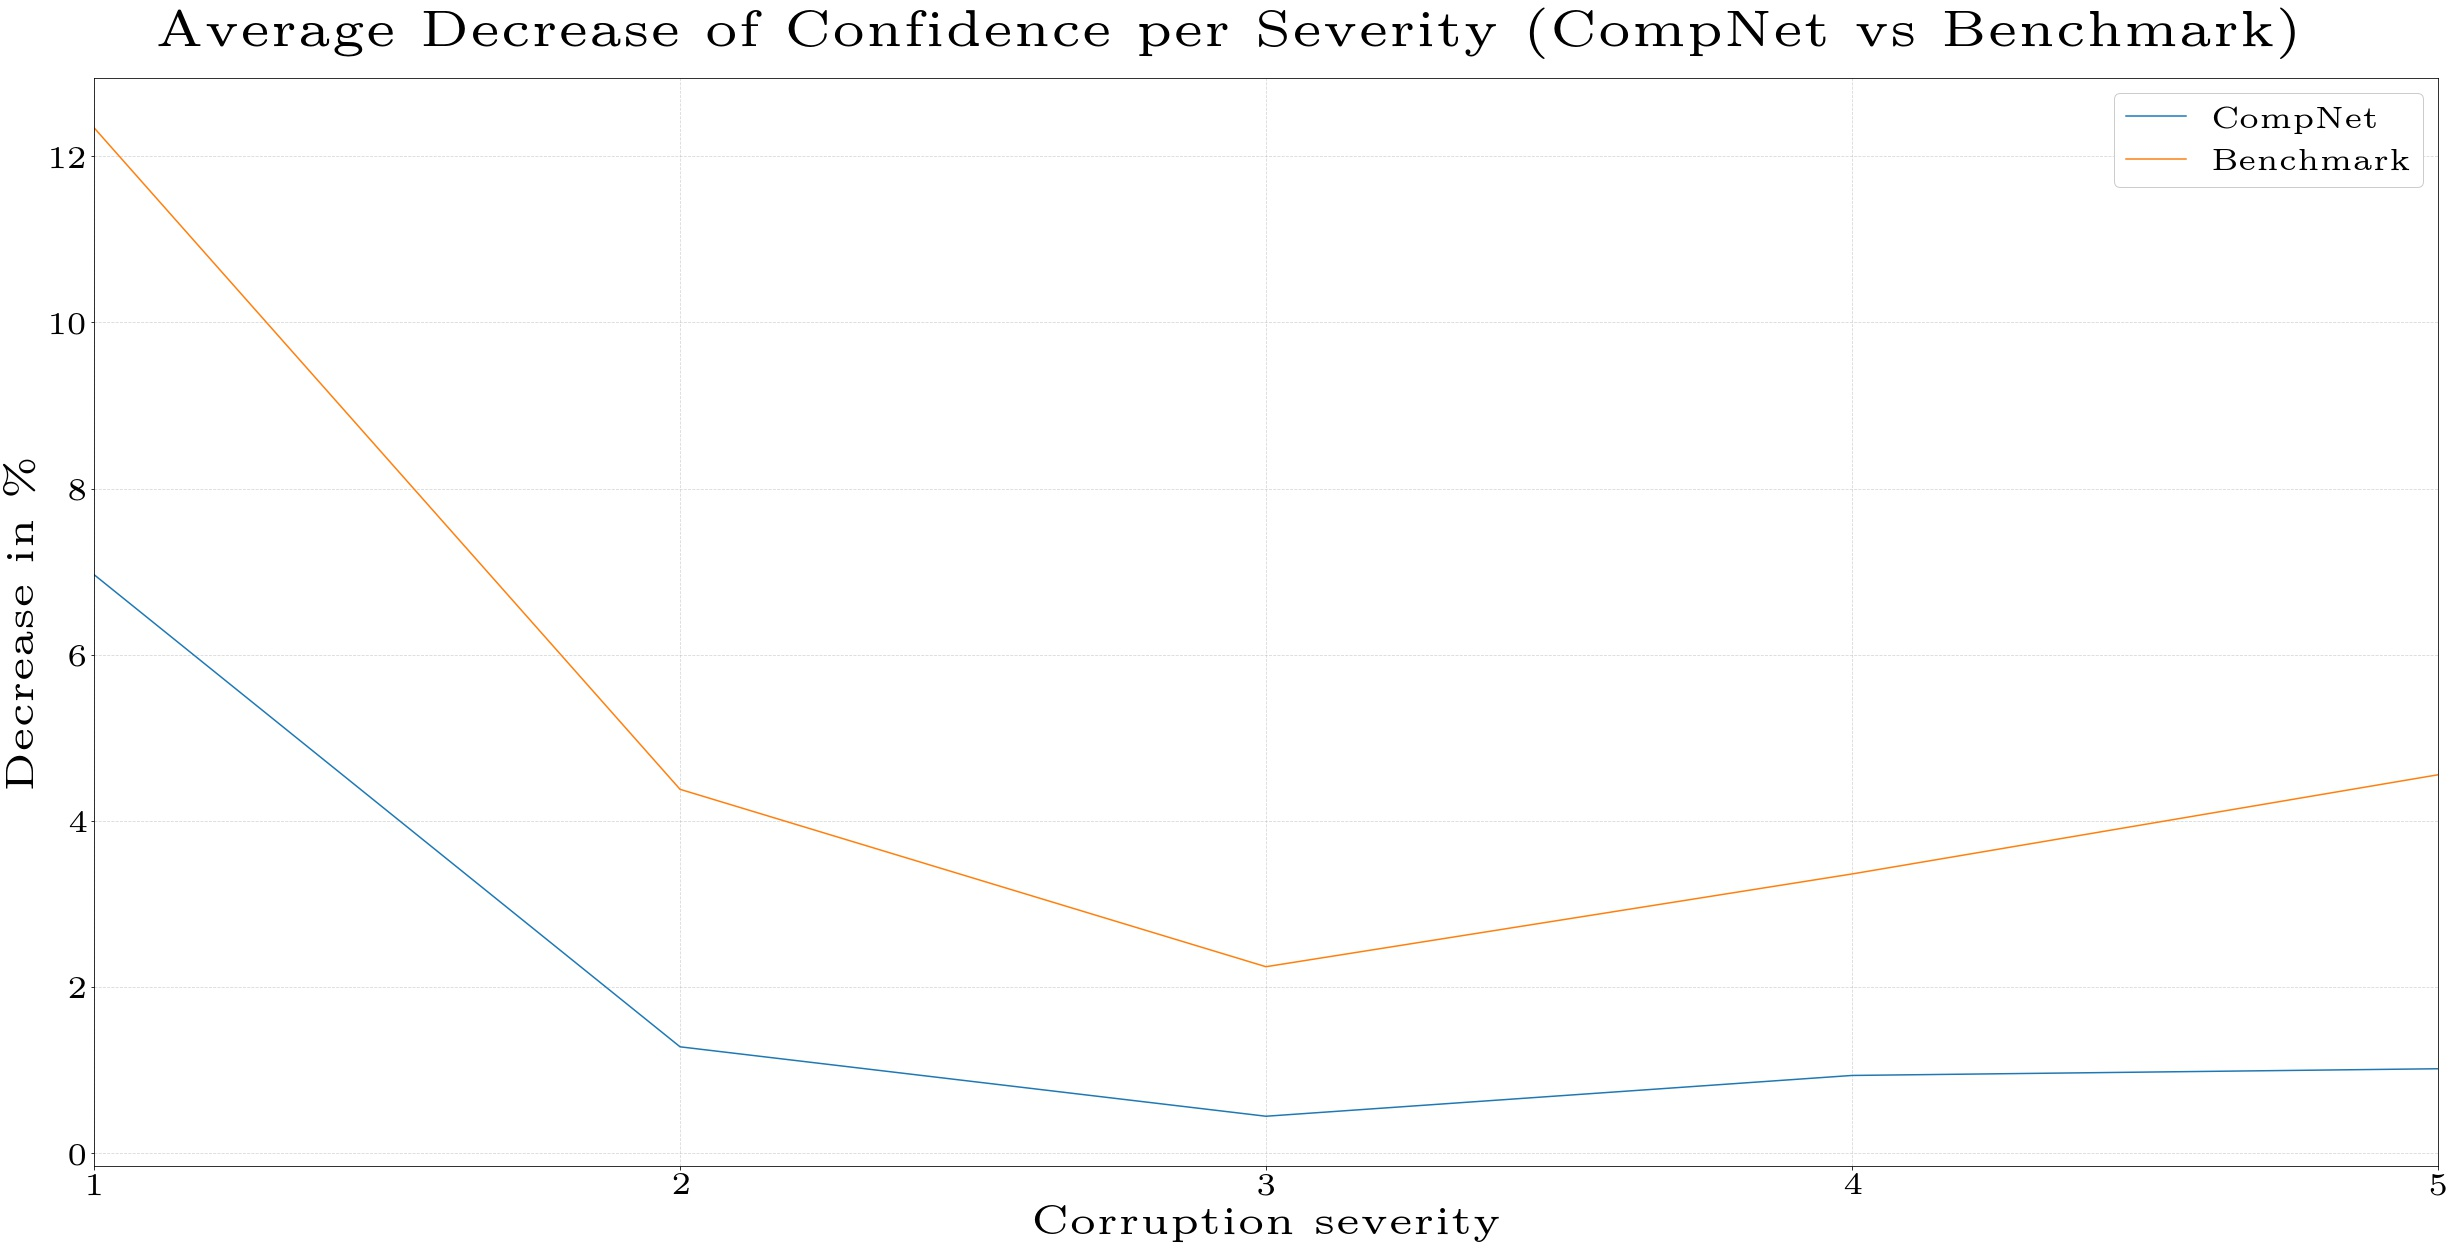
\includegraphics[width=\textwidth]{thesis/graphics/diagrams/uncertainty/uncertainty_compnet_benchmark_ds_confidence_decrease_print.jpg}
	    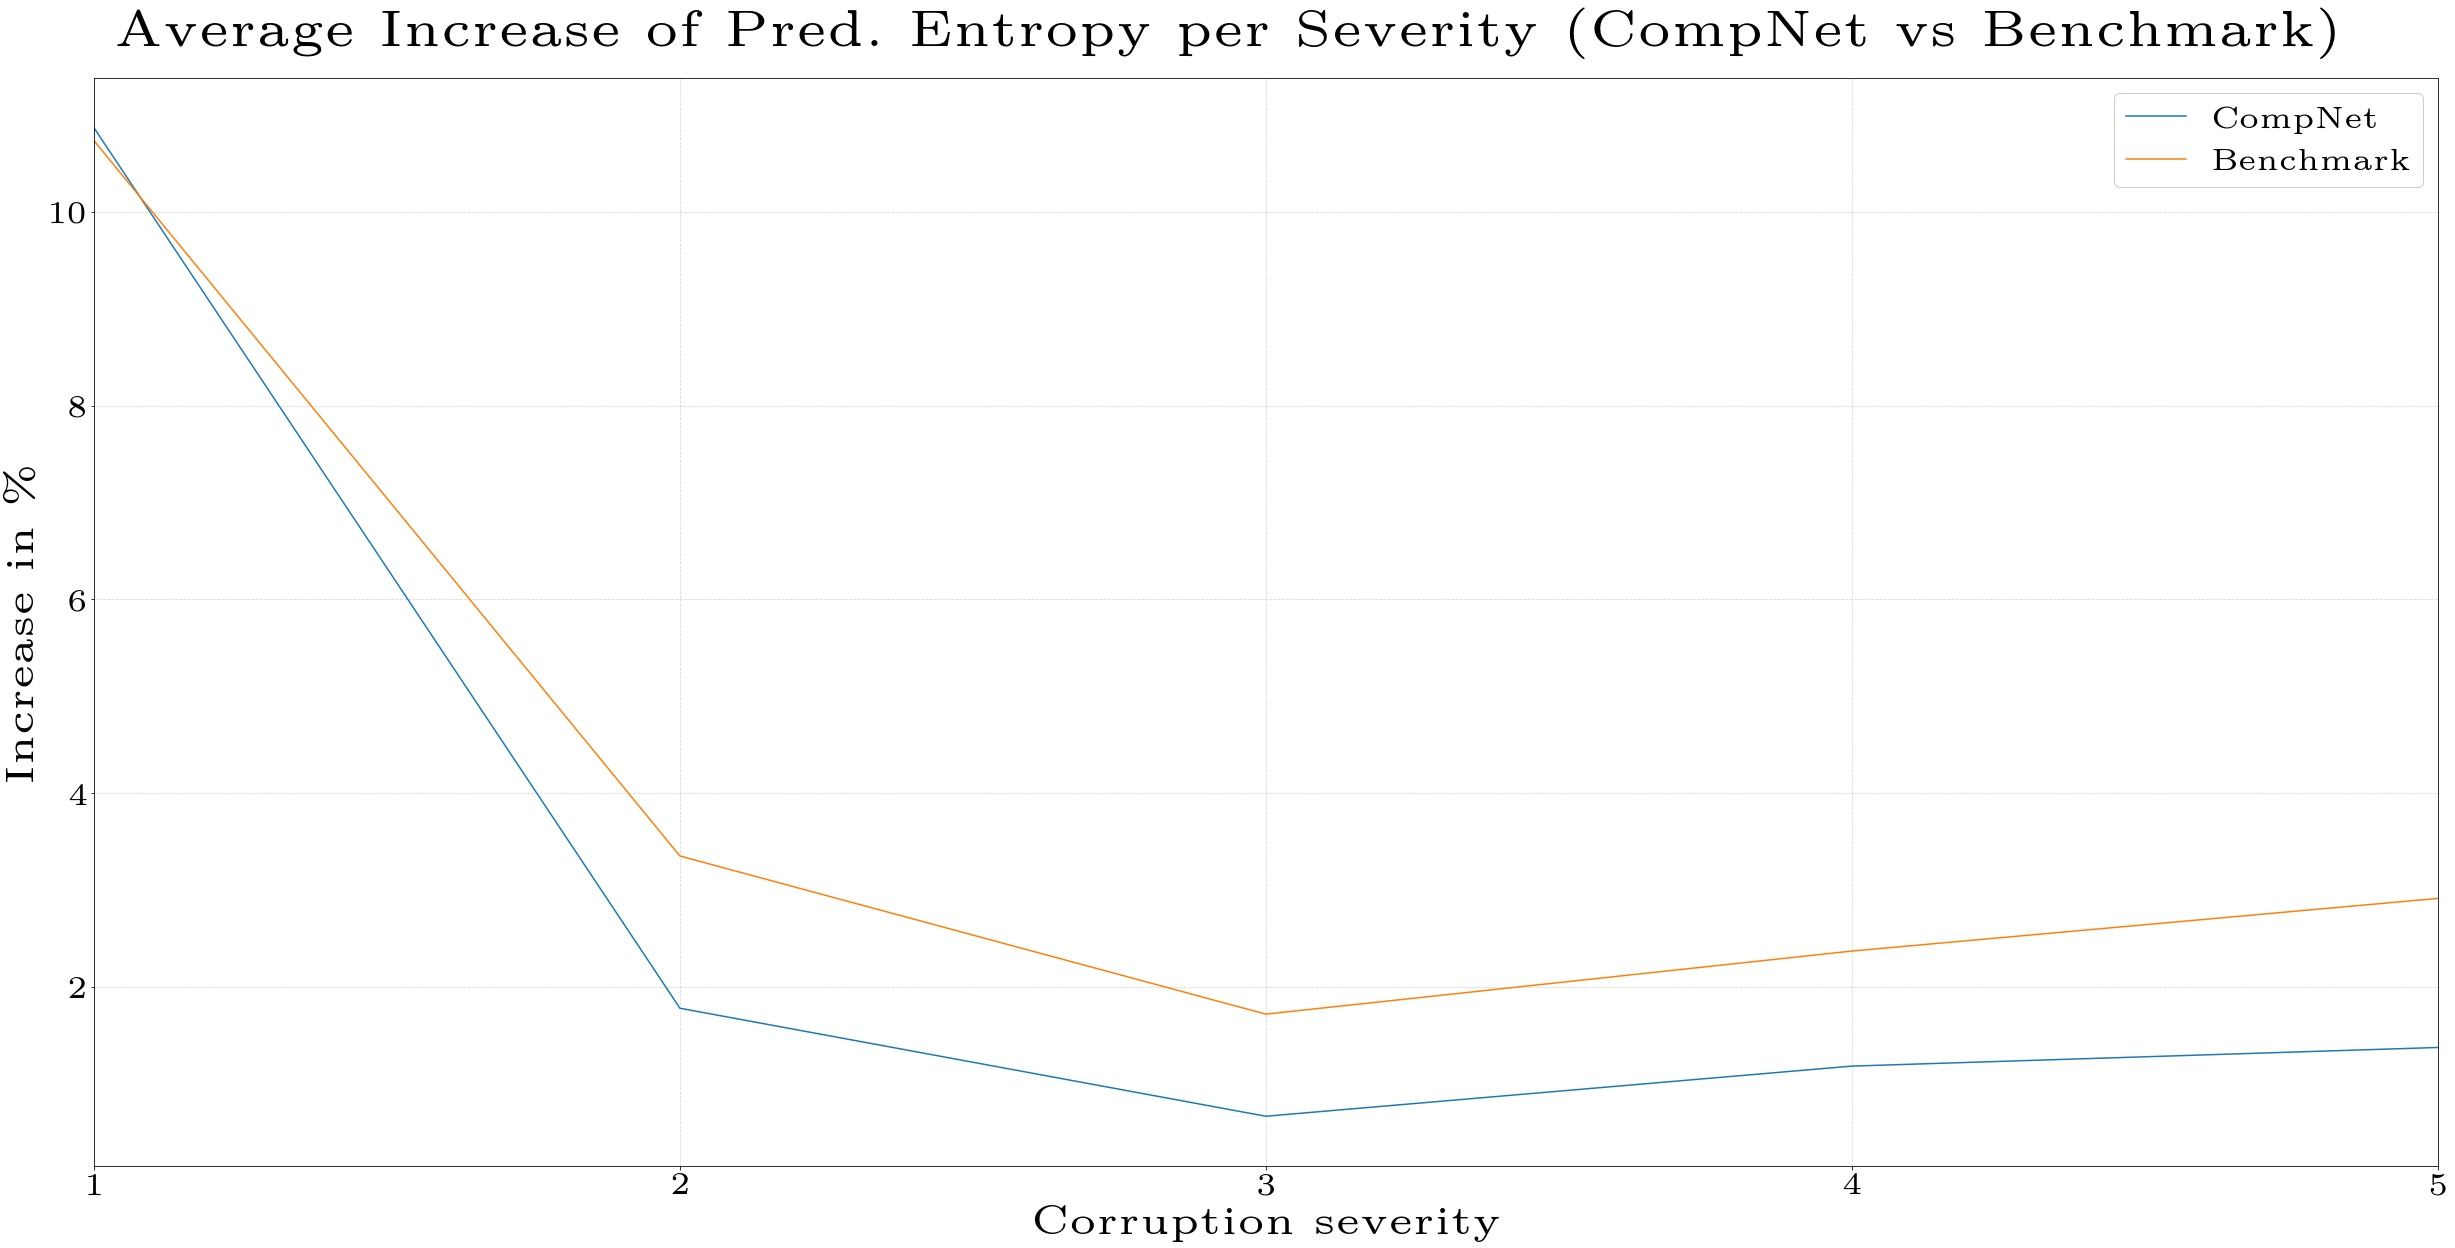
\includegraphics[width=\textwidth]{thesis/graphics/diagrams/uncertainty/uncertainty_compnet_benchmark_ds_pred_ent_increase_print.jpg}
    \caption{Development of different metrics with growing distributional data shift relative to the preceding severity level.}
    \label{fig:experiments_uncertainty_results_ds_metrics_development}
\end{figure}

\begin{figure}[htb]
    \centering
	    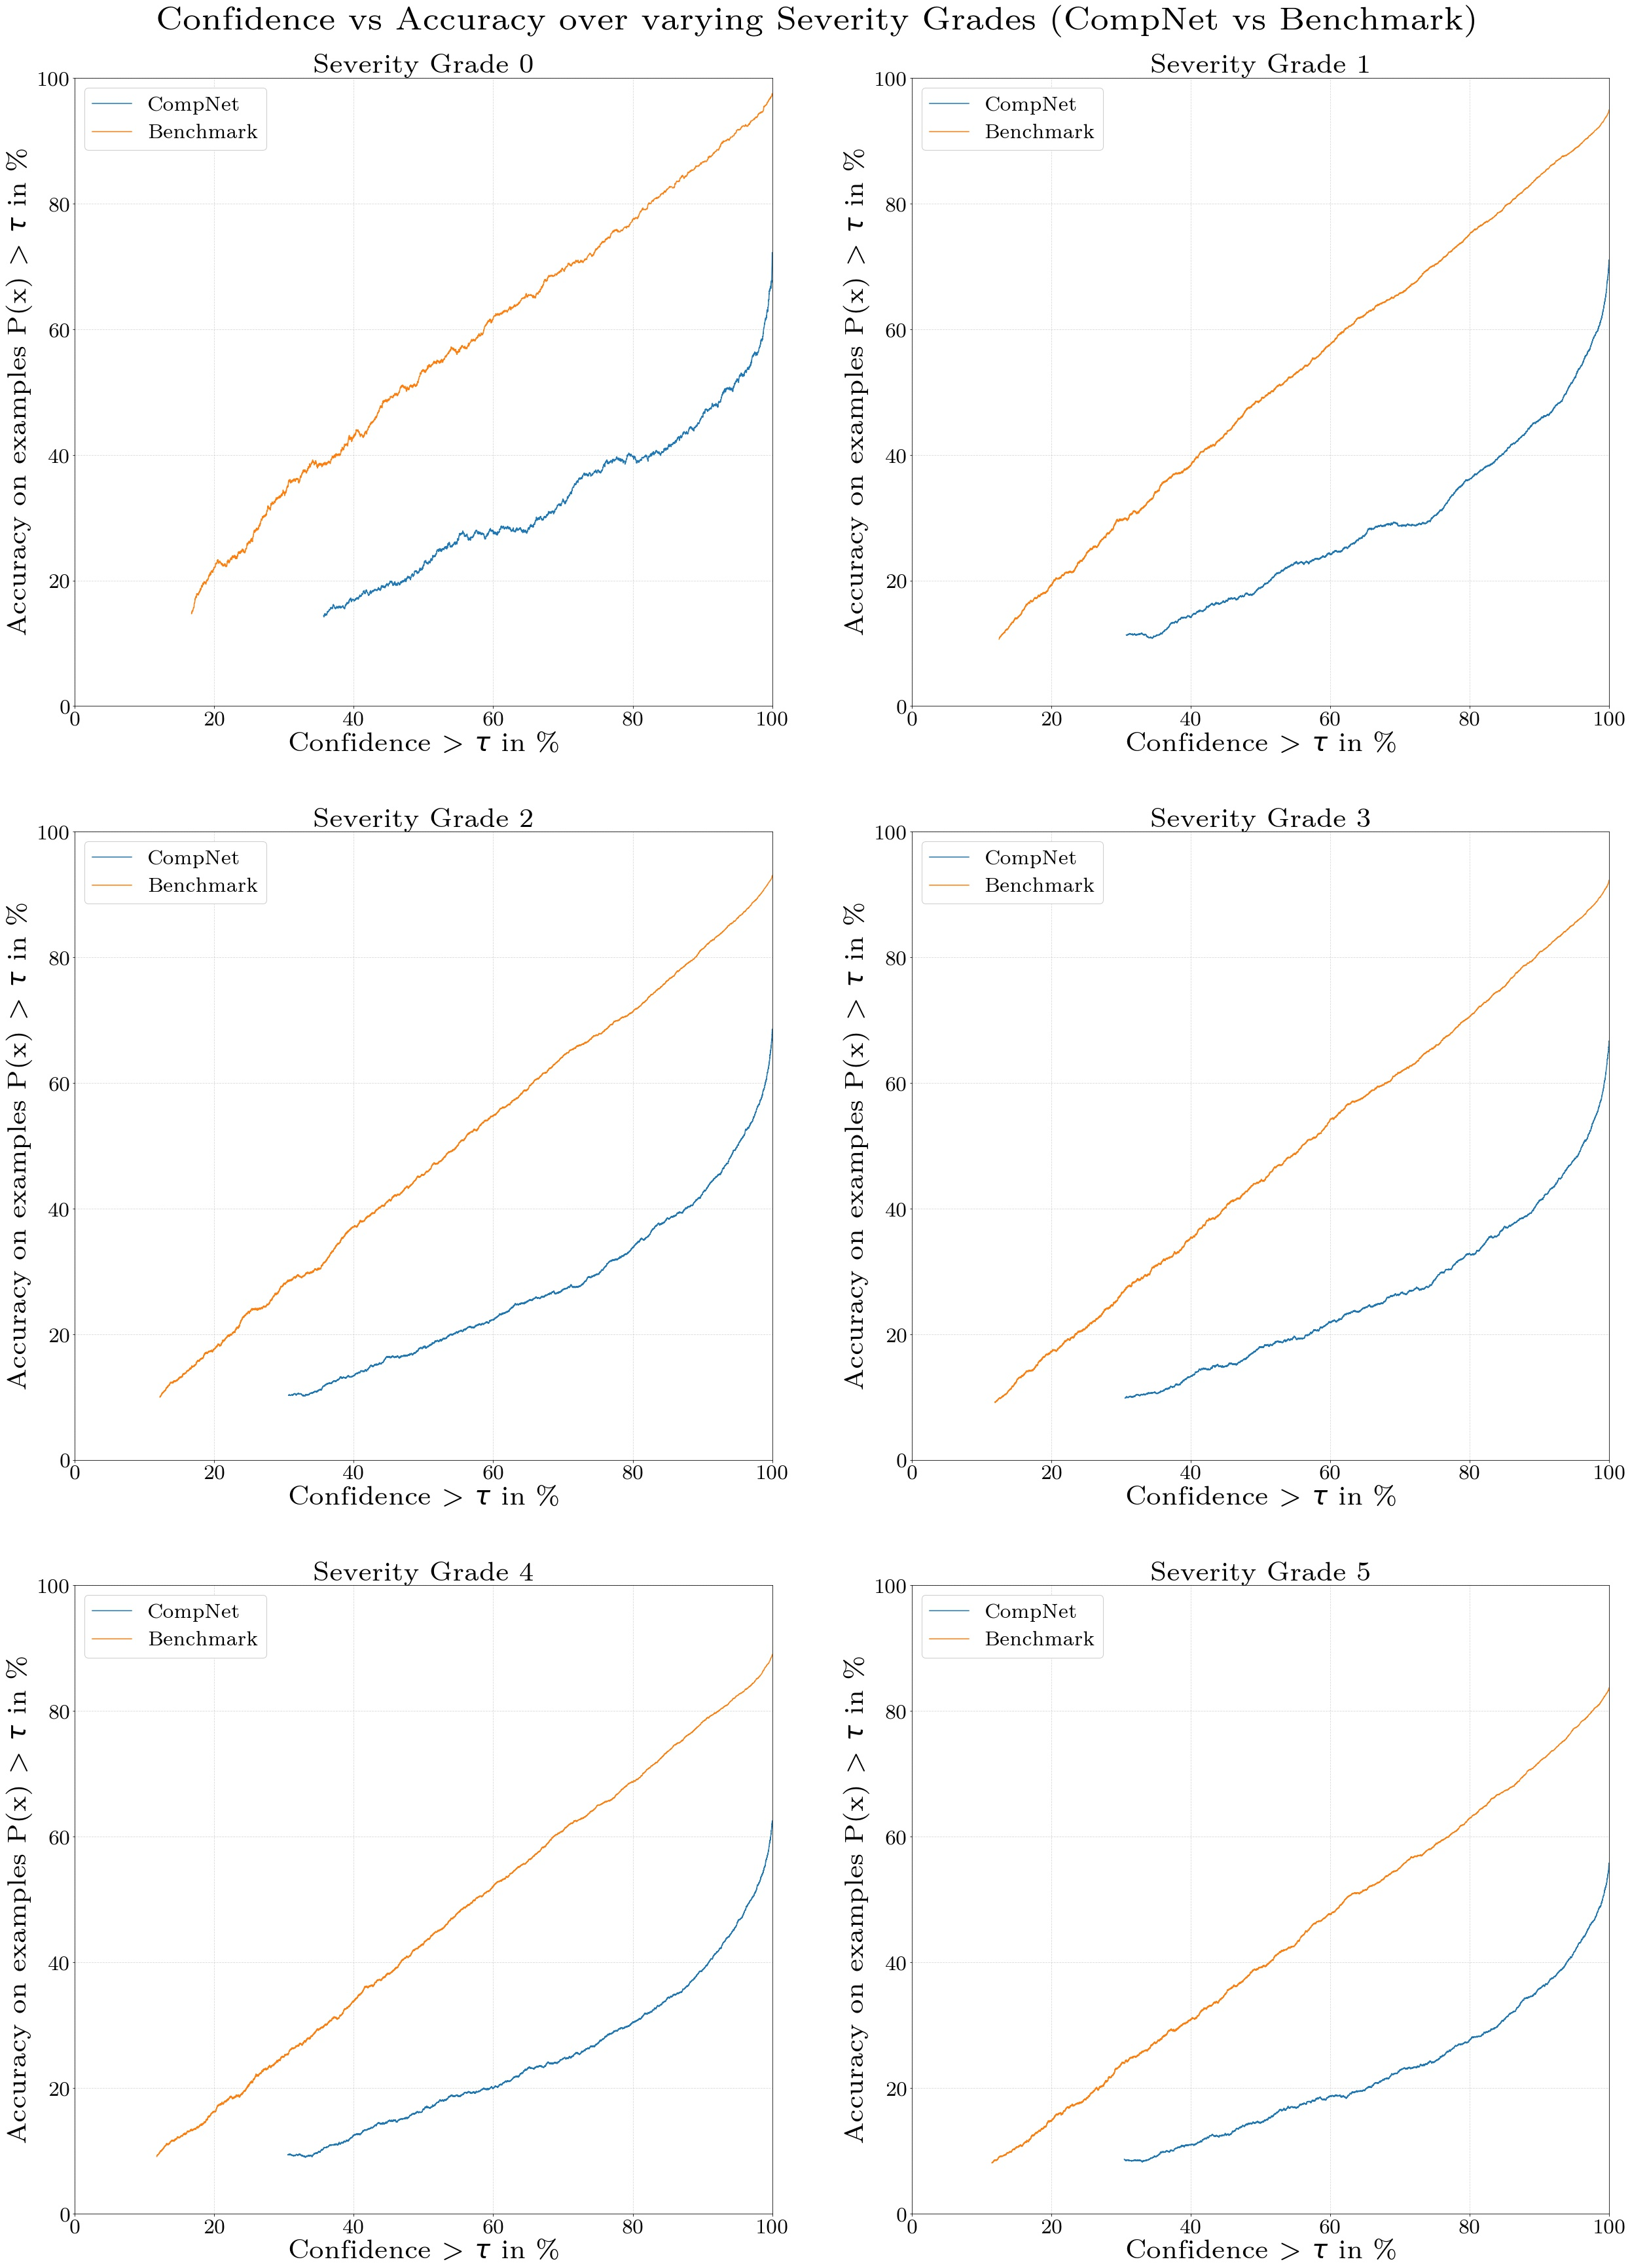
\includegraphics[width=\textwidth]{thesis/graphics/diagrams/uncertainty/uncertainty_compnet_benchmark_ds_confidence_accuracy_print.jpg}
    \caption{Development of confidence versus predictive accuracy for increasing corruption severities. As can be seen, the composed network is less well calibrated than the monolithic model. However, both deteriorate at a similar rate with growing distributional data shift.}
    \label{fig:experiments_uncertainty_results_ds_confidence_accuracy}
\end{figure}

\cleardoublepage

\section{Conclusion%
         \label{sec:conclusion}}

Modularization as a technique was evaluated to address several inherent shortcomings of DL and to improve the applicability of neural networks in practical scenarios. While many of the aspects discussed in sections \ref{sec:motivation} and \ref{sec:compnet} can be extended or abstracted to different areas of ML as well, this work solely focused on neural networks and particularly CNNs. Noteworthily, we consider our approach to be orthogonal (i.\,e.\ freely combinable and not obtrusive) to conventional performance-oriented methods.

The proposed technique was discussed at a conceptual level. Two different perspectives on modularization were presented and advantages and disadvantages of the approach were outlined. A theoretical foundation with regard to decomposable dimensions of ML models, convergence and performance properties of composed networks and different types of decomposition was established. Moreover, the concept of modularization errors was discussed in detail and a heuristic to estimate the impact of a specific form of decomposition on the performance of a model was provided.   

Exemplary experiments were conducted on different image recognition tasks to assess the technique's general viability as well as the qualitative impact it has on the model's behavior. Specifically, the overall performance and the robustness of composite networks were examined in a comparative juxtaposition with a monolithic reference model. Additionally, the propagation of modularization induced errors within decomposed models was evaluated for an exemplary network.

The results suggest the approach's validity. Generally, a decrease in performance proportional to the quality of the decomposition could be observed as a trade-off for desirable characteristics such as an increase in predictive cohesiveness (i.\,e.\ reduction of semantic distance of predictions) or simplified retrainability of individual submodules for composite networks. In particular the experiments on the ILSVRC2012 animal subset in section \ref{sec:experiments_imagenet} were able to demonstrate the advantage of modularized over monolithic models in early phases of the training.

Furthermore, it could be assessed that decomposed networks are not necessarily more susceptible to distributional data shift than conventional models. Rather, the findings discussed in section \ref{sec:experiments_uncertainty_results} suggest that while modularization induces a constant deterioration of the model's performance, it does not mandatorily impact the relative behavior of the underlying model. These conclusions, however -- similar to the other results -- do require further investigation as the scope of this work was limited to only specific forms of decomposition.

An additional insight obtained from the experiments is that (activation) functions of intermediate submodules that restrict the inter-modular informational flow such as \lstinline{max} or \lstinline{softmax} increase the modularization error. If possible, the use of these should be limited to the final output layer similar to conventional monolithic models.

Aside from these findings, this work once more demonstrated the necessity for a metric to measure the comparability of models. Even though it was decided to use the modeling capacity in terms of the number of DOFs for reference, there is, to our knowledge, no mathematical or quantitative foundation for the claim for this being the most eligible basis to compare neural networks on.

Regarding possible further research, this work opens the door for a multitude of interesting topics. Firstly, empirical investigations of other kinds of modularization mechanisms not assessed here such as Chaining or Additive and Multiplicative Aggregation are needed before final conclusions can be drawn concerning the universal validity of this technique. This is especially true with regard to the finding that decomposition does not influence the robustness and the overall behavior of a model. Additionally, it could be of interest to evaluate second-order networks composed from models different than neural networks or the performance of composite networks on tasks other than image recognition. An example could e.\,g.\ be contemporary NLP architectures that already inherently incorporate a composition of neural networks and autoencoders.

Another aspect worth investigating is the question of where to cut, i.\,e.\ how to find the optimal subspaces for the individual modules of a composite network. While in this work conceptually similar classes were grouped together in the experiments, it is not guaranteed that this is the best solution. For instance, the model may learn better if the individual categories per module were as diverse as possible instead. In this regard, unsupervised methods as e.\,g.\ proposed in \cite{Yan2015-go} could also be of interest.

Finally, there is the training routine for composite models. Considering the notion that the latter can be interpreted as second-order networks with module-level, dynamic (i.\,e.\ non-constant) nonlinearities presented in chapter \ref{sec:compnet_error_propagation}, it might be possible to transductively transfer the training algorithms for conventional neural networks, in particular backpropagation, to these systems. We hypothesize that the model could then be trained by either optimizing one submodule at a time while freezing the others or by interpreting all sub-search spaces as one composed space and optimize all modules at the same time instead of training each one independently as was done in this work. Albeit, as was mentioned before, this would necessitate backward traceability of the error flow through the meta-network and thus the gradient of the individual activation functions which is not necessarily given for module-level nonlinearities. However, it might e.\,g.\ be possible to approximate the local gradients of the submodules numerically via gradient quotient\footnote{A naive algorithm could e.\,g.\ slightly shift the inputs of each submodule for each forward-pass one at a time and calculate the gradient quotient from the resulting change at the output of the respective module. This is, however, computationally rather ineffective.}.

A noteworthy alternative that might be worth researching in this context is the RSO (Random Search Optimization) algorithm recently proposed by \cite{Tripathi2020-gc}. While not as computationally efficient as backpropagation, it has the advantage that it is more robust due to its stochastic nature and does not rely on the traceability of the error flow, hence also being applicable to non-parametric models.

On a final note, our current recommendation based on our findings is to modularize when necessary, but as little as possible to exploit the positive effects of the proposed technique while minimizing the increasing error induced by each further decomposition.

In conclusion, we do believe the presented approach possesses great potential, although from a practical rather than from a performance perspective. This work opens up a new perspective on existing approaches and provides the basis for a broad field of further research.

\cleardoublepage

\section{Acknowledgements}

We would like to thank Prof.\ Jörg Frochte for his supervision and guidance, as well as Kathrin and Uwe Friedrichsen for their massive support during the course of this work and for providing much needed feedback whenever necessary. Furthermore, we want to express our gratitude to Marcel Mikl, Philipp Stenkamp, Janis Mohr and Basile Tousside for helpful discussions.